%Description: In this latex document now biblatex will be used for bibliography. Therefore biber must be installed: $sudo apt-get install texlive-bibtex-extra biber. Additionally if change something on the document regarding to cites you have execute the custom command " Build with Biblatex" that contains the command $pdflatex %.tex | biber % | pdflatex %.tex | evince %.pdf. Otherwise a Quick Build with PdfLatex + View PDF would be sufficient.

\documentclass[11pt,a4paper]{report} %draft zeichnet nur rahmen für bilder -> performance

% Margin
\usepackage{setspace}
\usepackage{anysize}
\marginsize{3cm}{3cm}{2cm}{2cm}

\usepackage[utf8]{inputenc}
\usepackage[german]{babel}
\usepackage[T1]{fontenc}
\usepackage{amsmath}
\usepackage{amsfonts}
\usepackage{amssymb}
\usepackage{graphicx} %for logos and images
\usepackage{caption} %for logos and tables and figures
\usepackage{csvsimple} % for creating tables from csv file
\usepackage{subcaption} %for logos

%-----------------------------------------------------
\usepackage{listings} % used for source code listings
\lstdefinestyle{customc}{
  belowcaptionskip=1\baselineskip,
  breaklines=true,
  frame=single,
  numbers=left,   
  firstnumber=1,
  xleftmargin=1.8em,
  language=C,
  showstringspaces=false,
  basicstyle=\footnotesize\ttfamily,
  keywordstyle=\bfseries\color{green!40!black},
  commentstyle=\itshape\color{purple!40!black},
  identifierstyle=\color{blue},
  stringstyle=\color{orange},
  tabsize=2
}
\lstdefinestyle{customshell}{
  belowcaptionskip=1\baselineskip,
  breaklines=true,
  frame=single,
  numbers=left,   
  firstnumber=1,
  xleftmargin=1.8em,
  language=C,
  showstringspaces=false,
  basicstyle=\footnotesize\ttfamily,
  keywordstyle=\bfseries\color{green!40!black},
  commentstyle=\itshape\color{purple!40!black},
  identifierstyle=\color{blue},
  stringstyle=\color{orange},
  tabsize=2
}
\lstdefinestyle{custombinarycode}{
  frame=single,
  numbers=left,   
  firstnumber=1,
  numberfirstline=false,
  xleftmargin=2.5em,
  framexleftmargin=2.5em
}
%-----------------------------------------------------

\usepackage[svgnames]{xcolor} % color is used for background color in listings

%PassOptions with hyphens is used to correctly set line breaks on long urls. The url package is internally loaded by hyperref package!
\PassOptionsToPackage{hyphens}{url}\usepackage[colorlinks=true, linkcolor=Black,citecolor=Black,urlcolor=MidnightBlue]{hyperref} % for urls and hyperrefs -> use linkcolor to set a proper value for all links like DarkBlue or DarkGreen

%define new chapter format!
\usepackage{titlesec}
\titleformat{\chapter}[block]{\Huge\bfseries}{\thechapter}{15pt}{\Huge\bfseries}
\titleformat{\section}[block]{\normalfont\large\bfseries}{\thesection}{0.7em}{}
\titleformat{\subsection}[block]{\normalfont\normalsize\bfseries}{\thesubsection}{0.4em}{}
%
\usepackage{csquotes} % Recommended for biblatex in combination with babel
\usepackage[backend=biber,style=numeric,sorting=ynt]{biblatex}
\addbibresource{references.bib}

%use glossaries package to create an acronym listing
\usepackage[nonumberlist,nopostdot]{glossaries}
\makeglossaries % create makeindex files to sort acronyms. see glossaries package
\setacronymstyle{long-short}
\loadglsentries{acronyms}

%--------Start with document --------------------------------------------------------

\author{Johannes Busam}
\title{Masterthesis}
\date{01.09.2018}

\begin{document}
%\maketitle



\begin{titlepage}

\newcommand{\HRule}{\rule{\linewidth}{0.5mm}} % Defines a new command for the horizontal lines, change thickness here

\center % Center everything on the page
 
%----------------------------------------------------------------------------------------
%	HEADING SECTIONS
%----------------------------------------------------------------------------------------

\textsc{\LARGE Hochschule ...}\\[0.6cm] % Name of your university/college
\textsc{\Large Studiengang ...}\\ % Major heading such as course name

%----------------------------------------------------------------------------------------
%	TITLE SECTION
%----------------------------------------------------------------------------------------

\HRule \\[0.5cm]
{ \large \bfseries Masterthesis}\\[0.75cm] % Smaller one
{ \huge \bfseries Aufbau einer Plattform zur\\ forensischen Analyse basierend auf dem\\ Apache Hadoop\textsuperscript{\textregistered} Framework}\\[0.5cm] % Title
\HRule \\[0.5cm]
 
%----------------------------------------------------------------------------------------
%	AUTHOR SECTION
%----------------------------------------------------------------------------------------

\Large Zur Erlangung des akademischen Grades\\
\Large Master of Science\\[0.5cm] 

\Large vorgelegt im Sommersemester 2018\\[0.5cm] 

\Large von\\ Johannes Busam 

\begin{flushleft}
Erstbetreuung: ...\\[0.3cm] 

\noindent
Zweitbetreuung: ...\\

\end{flushleft}

\vfill % Fill the rest of the page with whitespace

\end{titlepage}

\pagenumbering{roman}
\setcounter{page}{2} %consider front page
% Kurzfassung, Abstract
%
\section*{Kurzfassung}
%Deutsch
TODO: Kurzfassung schreiben
%\gls{foam}\\

\newpage
\section*{Abstract}
%English
TODO: write abstract
\newpage

\section*{Danksagung}
TODO: Danksagung schreiben
\newpage

\section*{Eidesstattliche Erklärung}

Hiermit versichere ich an Eides statt, dass ich die vorliegende Arbeit selbstständig und
ohne Verwendung anderer als der angegebenen Hilfsmittel angefertigt habe. Alle Stellen,
die wörtlich oder sinngemäß aus veröffentlichten und nicht veröffentlichten Schriften
entnommen sind, sind als solche kenntlich gemacht. Die Arbeit hat in gleicher oder
ähnlicher Form noch in keiner anderen Prüfungsbehörde vorgelegen. Alle eingereichten
Versionen der Arbeit sind identisch.\\
\newline
\noindent
Meersburg, den XX.XX.2018 \\
\vspace{1.5cm} \\
Johannes Busam\newline

\newpage


\tableofcontents

\clearpage
\pagenumbering{arabic}
\setcounter{page}{1}

%----------------------------------------------------------------------------------------
%	Einleitung
%----------------------------------------------------------------------------------------

\chapter{Einleitung}
\label{ch:einleitung}

\section{Problemstellung}
Die forensische Analyse von digitalen Beweismitteln ist in der heutigen Zeit ein wichtiger Aspekt, um in der Strafverfolgung rechtswidriges Verhalten aufzudecken oder nachzuweisen. In vielen Fällen werden informationstechnische Systeme am Tatort gefunden oder zur Tatbegehung genutzt. Einschlägig sind hierbei Angriffe auf kritische Infrastrukturen durch Computersabotage oder das Ausspähen von Daten. Aber auch Urheberrechtsverletzungen durch die Weitergabe von geschützten Medien oder Verstöße gegen das Wettbewerbsrecht werden mit Informationstechnik begangen.
Je nach Dauer und Umfang der Strafhandlung werden gerade auch im Bereich der Wirtschaftskriminalität dutzende Asservate über informationstechnische Systeme erhoben. Beispielsweise werden beteiligte Computer und Mobiltelefone sichergestellt. Oder es werden logische Sicherungen von Netzwerkspeichern durchgeführt.\\

\noindent
Bei der Analyse dieser Asservate möchte ein forensischer Ermittler möglichst schnell einen Überblick über die sichergestellten Daten erhalten. Darauf aufbauend kann er entscheiden, welche Spuren in den Daten zum Nachweis konkreter Tathandlungen dienen und welche potentielle Beweismittel nicht weiter analysiert werden müssen.\\

\noindent
Der kritischste Aspekt hierbei ist, in kürzester Zeit die richtigen Informationen aus allen Daten zu extrahieren. Denn gerade in der Strafverfolgung ist eine schnelle und zielgerichtete Aufarbeitung der Ermittlungsfälle erforderlich. Darüber hinaus werden während der Analyse oftmals weitere Indizien gefunden, welche wiederum zur Sicherung neuer Beweismittel führen können. Je mehr Zeit jedoch für die Analyse benötigt wird, desto höher ist die Gefahr, dass noch nicht sichergestellte Daten endgültig gelöscht werden. Beispielsweise werden Telekommunikationsverbindungsdaten nicht über längere Zeiträume gespeichert.\\

\noindent
Zur Analyse stehen dem Forensiker etliche proprietäre und Open-Source Programme zur Auswahl. Allerdings sind im forensischen Open-Source Bereich viele Programme durch die Ressourcen des Analyserechners beschränkt. Sie bieten keine Möglichkeiten rechenintensive Aufgaben performant auf mehreren Computern zu skalieren.\\

\noindent
Aus fachlicher Sicht wäre eine Plattform sinnvoll, die anfallende Analyseaufgaben automatisiert auf allen Daten durchführt. Das System sollte die Ergebnisse unter Berücksichtigung verfügbarer Ressourcen schnellstmöglich ermitteln und dem forensischen Ermittler in einer aufbereiteten Form darstellen. Auf Basis dieser Ergebnisse könnte sich der Forensiker möglichst frühzeitig einen Überblick aller Beweismittel verschaffen, um dann bestimmte Daten auch in anderen spezialisierten Analyseanwendungen weiterzuverarbeiten. 

\section{Zielsetzung}
Zur Lösung der Problemstellung soll in dieser Masterthesis eine Plattform zur forensischen Analyse entwickelt werden. Diese Plattform soll durch eine automatisierte Analyse und Aufbereitung forensisch relevanter Informationen dem Forensiker helfen, sich einen Überblick zu verschaffen. Er soll dadurch effizient und zielgerichtet Datenanalysen durchführen können. Als Basis dieser Plattform soll das Apache Hadoop\textsuperscript{\textregistered} Framework genutzt werden. Hierbei sollen Vor- und Nachteile dieser Art der Datenverarbeitung im forensischen Kontext herausgearbeitet werden.\\ 

\noindent
Apache Hadoop ist ein etabliertes Open-Source Framework zur verteilten Speicherung und Verarbeitung von Daten. Durch die parallele Datenverarbeitung eignet sich ein Hadoop-Cluster auch zu Prozessierung von großen Datenmengen im Terabyte-Bereich. Ein zugrunde liegendes Paradigma ist hierbei, dass die Programmausführung dort stattfindet wo auch die Daten liegen, um kostspielige Datentransporte weitgehend zu vermeiden. Aufgrund dieser Beschaffenheit könnte diese Art der Datenverarbeitung auch Geschwindigkeitsvorteile bei forensischen Analysen bieten. \\

\noindent
Ein wichtiger Aspekt der Masterthesis ist die Aufbereitung der Daten für die Analyse im Hadoop-Cluster. Hierbei sollen mehrere Möglichkeiten analysiert werden, wie diese Aufbereitung und Speicherung der Daten im Hadoop-Cluster gelingen kann. Dabei muss auch auf die Unversehrtheit der Dateiinhalte und Metadaten bei der Aufbereitung geachtet werden. Darauf aufbauend soll eine fachliche Verwaltungsstruktur entwickelt werden, die es auch erlaubt mehrere Asservate von beliebigen Ermittlungen parallel zu verarbeiten. Dadurch können auch Zusammenhänge zwischen unterschiedlichen Asservaten identifiziert werden.\\

\noindent
Im Rahmen der Thesis soll die Datenanalyse vorerst grundlegende Funktionen unterstützten.
So sollen die Metadaten, wie beispielsweise Name, Dateipfad, Hashsumme, Dateityp, Größe und Zeitstempel ermittelt werden und zu weiteren Analysen zur Verfügung stehen.
Es soll auch eine Volltextsuche auf den Daten möglich sein. Darauf aufbauend soll der Nutzer beispielsweise gleiche Dateien und Verbindungen zwischen den einzelnen Beweismitteln erkennen können.
Optional könnte die Analyseplattform gezielt nach IP-Adressen, Web-Adressen, E-Mail-Adressen oder Positionsdaten\footnote{Beispielsweise könnten Geopositionen oder Ortsnamen aus Dateien extrahiert werden. Diese Daten könnten dann mit ihrem geografischen Bezug auf einer Karte dargestellt werden.} suchen.\\

\noindent
Die Resultate durchgeführter Datenanalysen sollen dem Nutzer bereitgestellt werden. Hierzu
wird eine grafische Oberfläche benötigt, welche die fachlichen Aspekte der forensischen Analyseplattform widerspiegelt. Im Rahmen der Thesis sollen Möglichkeiten analysiert werden, wie eine grafische Oberfläche aussehen könnte. In diesem Kontext soll auch geprüft werden, ob existierende Programme zur Datenvisualisierung im Hadoop-Umfeld wiederverwendet werden könnten. Die Implementierung einer grafischen Oberfläche ist im Rahmen dieser Thesis jedoch nicht angedacht.\\

\noindent
Abbildung \ref{fig:foam_analysis_approach} skizziert das angestrebte Analysevorgehen mit dieser Analyseplattform. Der Forensiker soll digitale Beweismittel in das Hadoop-Cluster importieren können. Nachfolgend hat er die Möglichkeit diverse Analysen auf den Daten durchzuführen. Die Ergebnisse könnten später über eine entsprechende Oberfläche visualisiert werden.\\

\begin{figure}[ht]
  \centering
  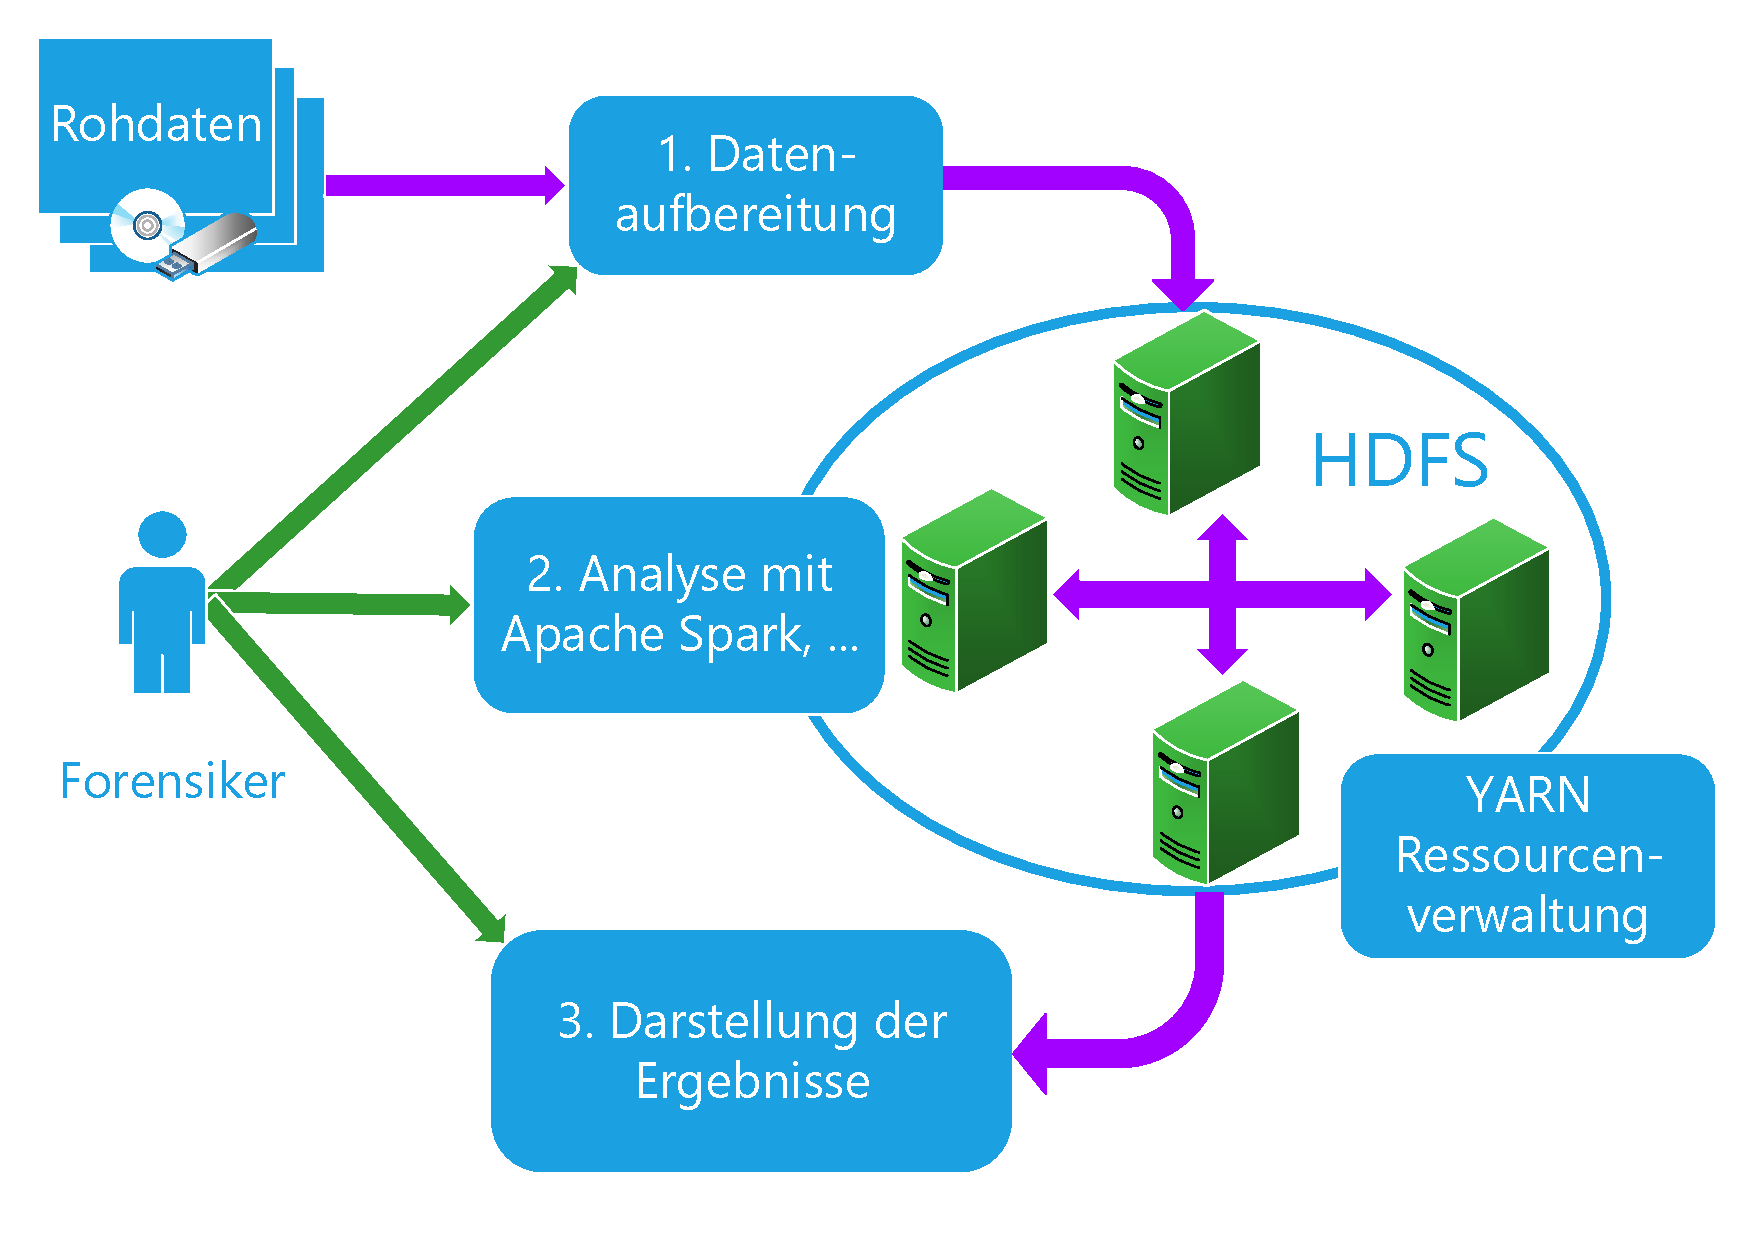
\includegraphics[width=0.82\textwidth]{./resource/Hadoop-Struktur.pdf}
  \caption{Analysevorgehen}
  \label{fig:foam_analysis_approach}
\end{figure}

\noindent
Das Ziel dieser Masterthesis ist es, dem forensischen Ermittler schnellstmöglich einen Überblick zu den einzelnen Beweismitteln und deren Zusammenhänge im Kontext einer Fallanalyse zu liefern. \\

\noindent
Bei einer realen forensischen Analyse gibt es weitere Anforderungen, die das Analysesystem erfüllen sollte. Da in vielen Fällen hochsensible personenbezogene Daten und Geschäftsgeheimnisse verarbeitet werden, müssen auch entsprechende Regelungen getroffen werden, wie nach der Analyse alle Daten restlos aus dem System gelöscht werden können.\\
Das System muss gegen fremden Zugriff gesichert sein. Es muss zu jeder Zeit ersichtlich sein, welche Personen zu welchem Zweck auf das System zugreifen.\\
Ein weiterer Aspekt in der Analyse ist die lückenlose Erstellung einer Beweismittelkette (Chain of Custody). Für jedes forensische Analyseergebnis müssen die Herkunft und die Verarbeitungsschritte transparent nachvollziehbar sein.\\
Im Rahmen der Masterthesis soll diese Aspekte zumindest theoretisch und wenn möglich auch praktisch analysiert werden.\\

\noindent
Aus organisatorischer Sicht soll die Analyseplattform als Open Source Projekt bereitgestellt werden. Hierzu soll der Source-Code, die Konfiguration des Systems und die Dokumentation in einer öffentlich zugänglichen Versionsverwaltung verfügbar sein.\\


\clearpage
\section{Aufbau}
In Kapitel \ref{ch:einleitung} wird das Eingangsproblem und die Ziele dieser Masterthesis beschrieben.\\ 
In Kapitel \ref{ch:development_approach} folgt das allgemeine Entwicklungsvorgehen. Darin ist der aktuelle Projektplan enthalten, welcher die Arbeitspakete definiert.
Zusätzlich wird die genutzte Entwicklungsumgebung skizziert.\\

\noindent
In Kapitel \ref{ch:theory_hadoop} erfolgt eine Darstellung der Apache Hadoop Plattform inklusive theoretischen Grundlagen zur Arbeitsweise des Frameworks. Des Weiteren werden darauf aufbauende Projekte, wie beispielsweise Apache Spark und Apache HBase erklärt.\\

\noindent
In Kapitel \ref{ch:data_persistence} werden unterschiedliche Varianten zur Datenspeicherung und Aufbereitung analysiert. Innerhalb dieses Kapitels wird eine Möglichkeit entwickelt, wie die Daten eines Asservats im Hadoop-Cluster gespeichert werden können, um sie später parallelisiert verarbeiten zu können. Zu Beginn wird das herkömmliche Analysevorgehen in Verbindung mit der Analyseanwendung \textit{Autopsy} beschrieben, um fachlich relevante Aspekte bei der Analyse herauszuarbeiten.\\

\noindent
Die eigentliche Datenverarbeitung wird Kapitel \ref{ch:data_processing} beschrieben. Hier wird ein Ansatz vorgestellt, wie die Daten parallel verarbeitetet werden können. Anhand dieses Ansatzes werden Hashsummen der Daten berechnet und die Medientypen der Dateien ermittelt. Zum Schluss wird eine Möglichkeit vorgestellt, wie die Informationen für eine Volltextsuche aufbereitet werden können.\\

\noindent
In Kapitel \ref{ch:additional_aspects} werden querschnittliche Aspekte zur Datensicherheit und zur Beweismittelkette von forensischen Analysen skizziert.\\

\noindent
Die Visualisierung der Informationen ist ein interessanter Aspekt der forensischen Analyseplattform, welcher in Kapitel \ref{ch:data_visualization} beschrieben wird. Dort werden einige Möglichkeiten erläutert, wie eine Visualisierung aussehen könnte.\\

\noindent
In Kapitel \ref{ch:result_discussion} werden die gewonnen Ergebnisse dieser Masterthesis kritisch hinterfragt. Hierbei wird geprüft, ob die Erwartungen an eine performante Datenaufbereitung und Analyse erfüllt werden. Es wird auch aufgezeigt, ob das Apache Hadoop Framework überhaupt die Anforderungen einer forensischen Analyseplattform erfüllen kann.\\   

\noindent
Zuletzt erfolgt in Kapitel \ref{ch:zusammenfassung} eine Zusammenfassung der erarbeiteten Ergebnisse. Offene Punkte und Verbesserungen des Systems werden in Kapitel \ref{ch:ausblick} diskutiert. 

\chapter{Vorgehen}
\label{ch:development_approach}

\section{Projektplanung}
\label{sec:project_plan}
Zur Realisierung einer forensischen Analyseplattform wurde ein Projektplan erstellt, welcher die einzelnen Aufgaben im Rahmen der Masterthesis enthält. Abbildung \ref{fig:workpackages} zeigt die Aufteilung in diese Arbeitspakete.\\
Das Ziel der Einarbeitungsphase ist, ein grundlegendes Verständnis über die Datenverarbeitung im Hadoop-Framework zu erhalten. Zusätzlich soll eine Entwicklungsumgebung inklusive öffentlicher Versionsverwaltung eingerichtet werden. Danach erfolgt der Aufbau eines eigenen Hadoop-Clusters und die Beschaffung von Testdaten.\footnote{Hierbei wird ein bestehendes Hadoop-Cluster genutzt und um zusätzliche Softwarepakete ergänzt.} Für die Einarbeitung und den Aufbau sind vier Wochen eingeplant (siehe Abbildung \ref{fig:ganttA}).\footnote{Die referenzierten Gantt-Diagramme wurden mit der JavaScript-Bibliothek \textit{dhtmlxGantt} erstellt. Der Quellcode ist unter der \textit{GNU GPLv2}-Lizenz lizenziert. Weiter Informationen können in Kapitel \ref{sec:licencing_issues} im Anhang nachgelesen werden.}\\

\noindent
Der zweite Teil behandelt die Datenaufbereitung und Speicherung im Hadoop-Cluster. Es soll geprüft werden, welche Struktur der Daten für eine optimale Speicherung und Verarbeitung im Hadoop-Framework erforderlich ist. Für diesen Teil sind vier Wochen Bearbeitungszeit geplant.\\
Am Ende des Arbeitspakets soll ein erster Zwischenbericht erstellt werden, welcher die bisherigen Ergebnisse enthält (sieh Abbildung \ref{fig:ganttA}).\\

\begin{figure}[ht]
  \centering
  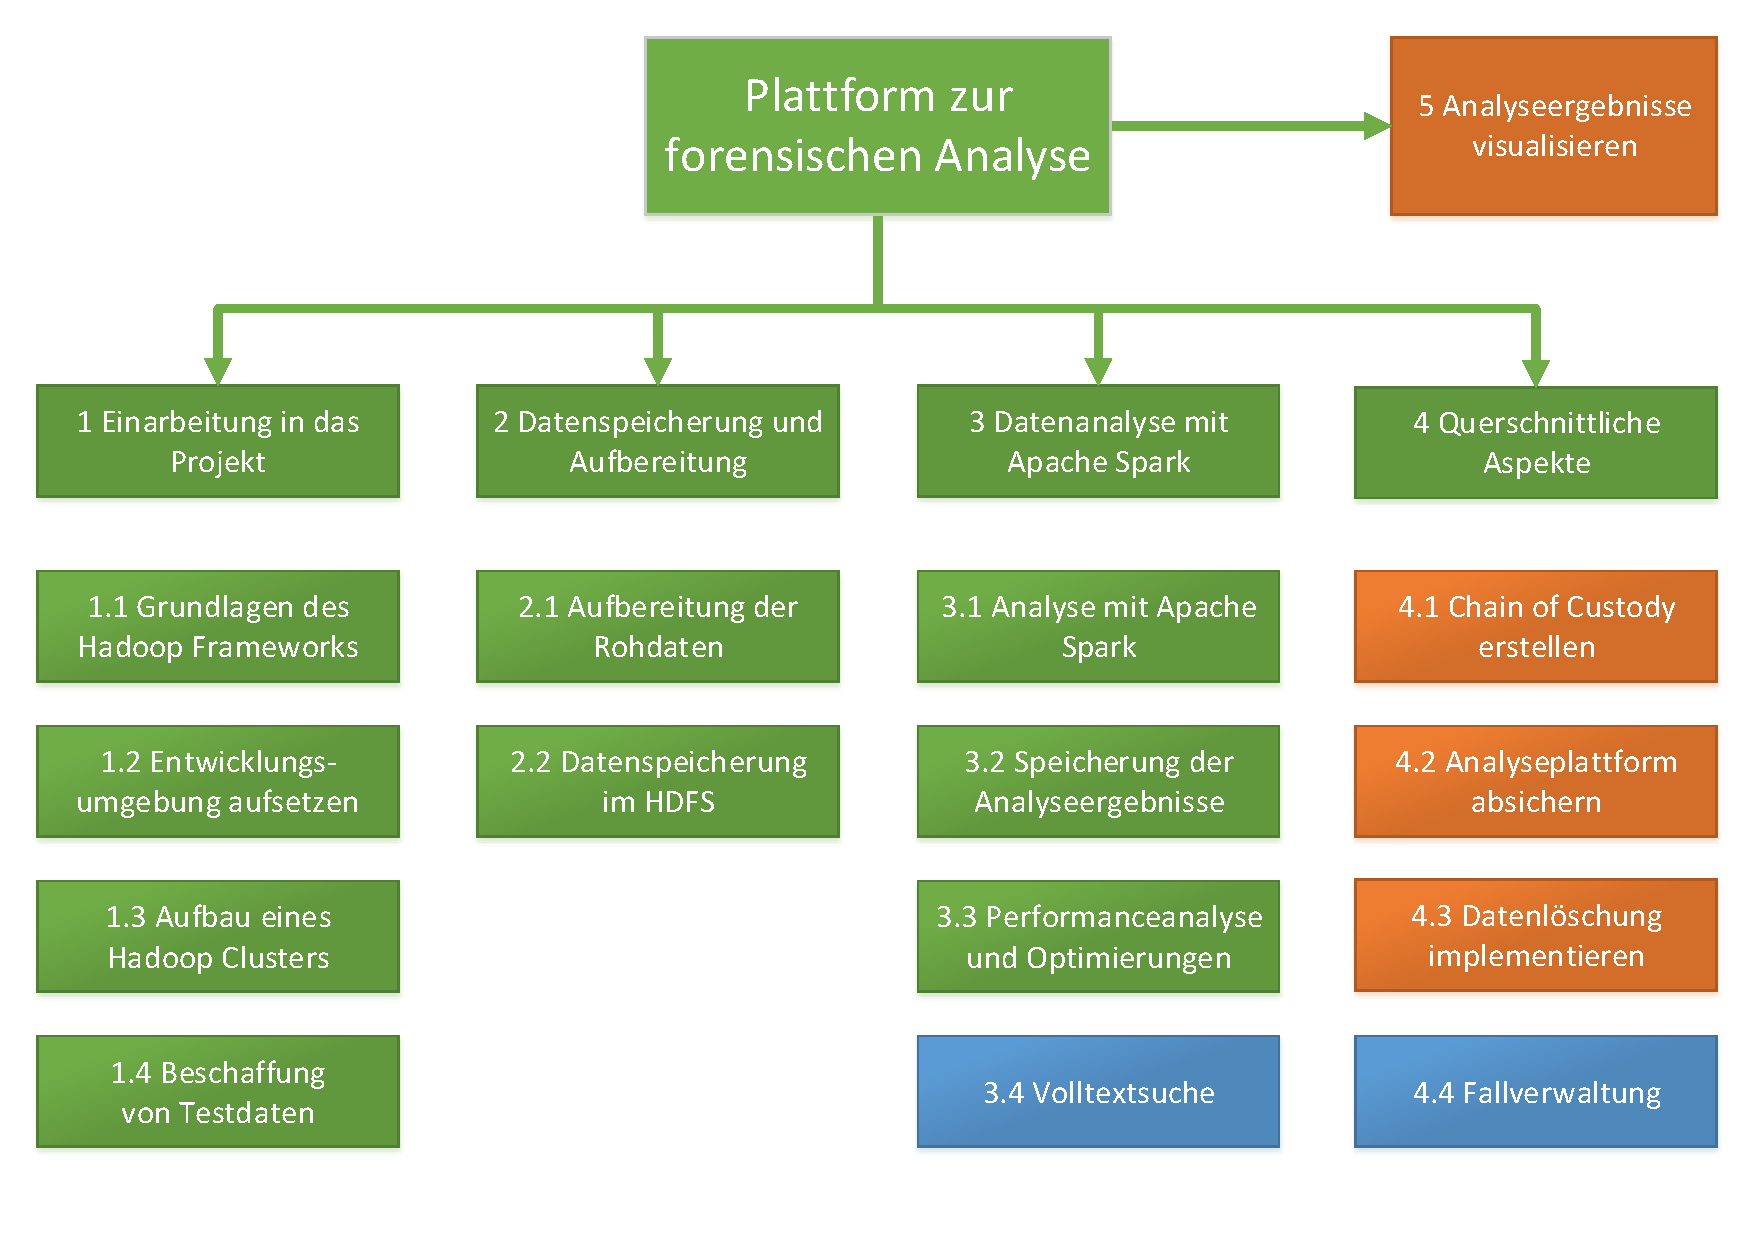
\includegraphics[width=\textwidth]{./resource/Arbeitspakete.pdf}
  \caption{Arbeitspakete der Masterthesis}
  \label{fig:workpackages}
\end{figure}

\noindent
Nach der Speicherung der Rohdaten erfolgt im dritten Arbeitspaket die Datenanalyse mit Apache Spark. Hier sollen die Daten nach anwendungsbezogenen Problemstellungen analysiert werden. Ein weiterer Aspekt der Datenanalyse beschäftigt sich mit den Möglichkeiten, wie die Ergebnisse persistiert werden können.\footnote{Dafür soll Apache HBase zur Speicherung von strukturierten und unstrukturierten Daten untersucht werden.}Im Anschluss soll die Performanz der Algorithmen geprüft werden. Hier bietet sich der Vergleich zu herkömmlichen Analyseprogrammen an. Denn schließlich hat diese Thesis auch das Ziel, bei großen Datenmengen schneller Ergebnisse zu liefern als die herkömmlichen Analysewerkzeuge auf einem einzelnen Analyserechner. Für dieses Arbeitspaket sind sieben Wochen eingeplant (siehe Abbildung \ref{fig:ganttB}).\\
 Darauf folgt ein zweiter Zwischenbericht.\\

\noindent
Im letzten Drittel der Masterthesis sollen querschnittliche Aspekte in die bestehende Analyseplattform integriert werden. Hierbei geht es um das Absichern der Plattform, die Dokumentation der Beweismittelkette und um das sichere Löschen von Asservaten. Für dieses Arbeitspaket sind vier Wochen eingeplant (siehe Abbildung \ref{fig:ganttC}).\\

\noindent
Das letzte Arbeitspaket enthält ein prototypische Visualisierung der Analyseergebnisse. Hierbei soll geprüft werden, welche Möglichkeiten zur Darstellung der Ergebnisse existieren. Für diese Arbeit sind drei Wochen eingeplant (siehe Abbildung \ref{fig:ganttC}).\\

\subsection*{Projektverlauf}
Während dem Projektverlauf wurde die Planung teilweise angepasst. Es wurden einige Aspekte aus der Planung entfernt (orange hinterlegt in Abbildung \ref{fig:workpackages}). So wurden die Visualisierung der Ergebnisse, die Erstellung der Beweismittelkette, das Absichern der Analyseplattform und die forensisch korrekte Datenlöschung nicht implementiert sondern nur theoretisch erläutert. Der Hauptgrund dafür, war eine intensive Analyse und Entwicklung, wie die Daten im Hadoop-Cluster gespeichert werden können. Hier wurden mehrere Varianten getestet und die ursprünglich angedachte Bearbeitungszeit verlängerte sich.\\

\noindent
Andererseits sind auch neue Arbeitspakete hinzugekommen (blau hinterlegt in Abbildung \ref{fig:workpackages}). So wurde bei der Datenanalyse mit Apache Spark sichtbar, dass die Informationen und Analyseergebnisse performant durchsuchbar sein müssen. Daher wurde untersucht, wie eine Volltextsuche aller gespeicherten Daten im Hadoop-Cluster realisiert werden könnte.\\
Ein anderer Aspekt ist die Implementierung einer Fallverwaltung. Denn damit können nun mehrere Asservate in das System importiert werden, um Zusammenhänge identifizieren zu können. 

\begin{figure}[p]
  \centering
  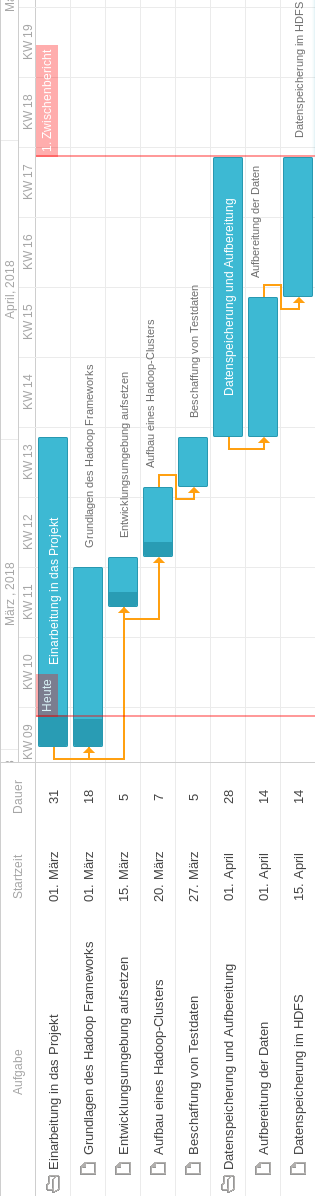
\includegraphics[width=\textwidth,height=\textheight,keepaspectratio]{./resource/ganttA.png}
  \caption{Projektplan Teil A - Einarbeitung und Rohdatenspeicherung (siehe Kapitel \ref{sec:licencing_issues})}
  \label{fig:ganttA}
\end{figure}

\begin{figure}[p]
  \centering
  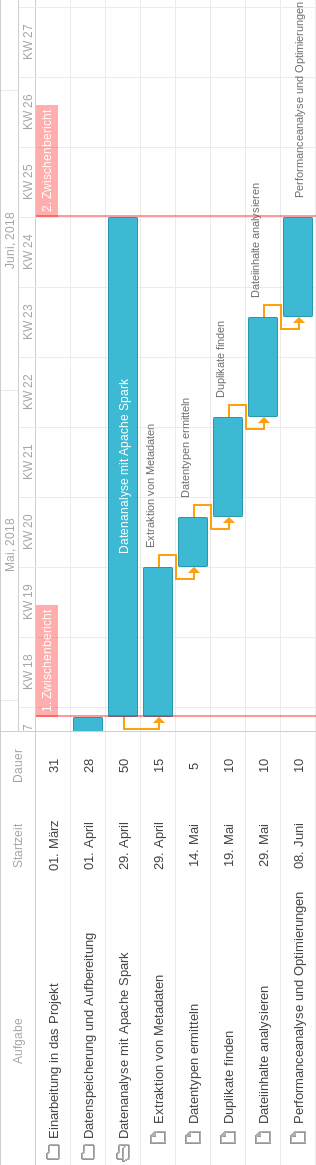
\includegraphics[width=\textwidth,height=\textheight,keepaspectratio]{./resource/ganttB.png}
  \caption{Projektplan Teil B - Datenanalyse (siehe Kapitel \ref{sec:licencing_issues})}
  \label{fig:ganttB}
\end{figure}

\begin{figure}[p]
  \centering
  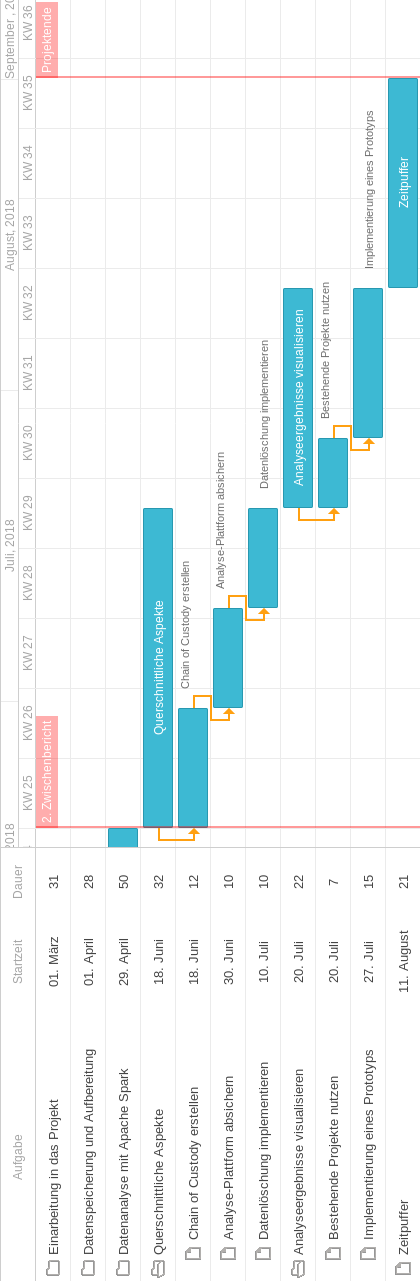
\includegraphics[width=\textwidth,height=\textheight,keepaspectratio]{./resource/ganttC.png}
  \caption{Projektplan Teil C - Querschnittliche Aspekte und Visualisierung (siehe Kapitel \ref{sec:licencing_issues})}
  \label{fig:ganttC}
\end{figure}

\clearpage
\section{Entwicklungsumgebung}
\label{development_environment}
Der Aufbau eine Test- und Entwicklungsumgebung ist ein wichtiger Bestandteil dieser Thesis. Einerseits sollen Anwendungsprogramme zur Datenverarbeitung schnell und lokal ausführbar sein. Andererseits soll die Testumgebung auf einem physikalischem Apache Hadoop Cluster basieren, um mögliche Infrastrukturprobleme identifizieren zu können und die Performanz zu testen. \\

\noindent
Abbildung \ref{fig:development_environment} skizziert die Komponenten der Entwicklungsumgebung. Zentraler Bestandteil ist ein Entwicklungsrechner mit der Linux-Distribution \textit{Fedora} in der Version 28 64-bit.

\begin{figure}[ht]
  \centering
  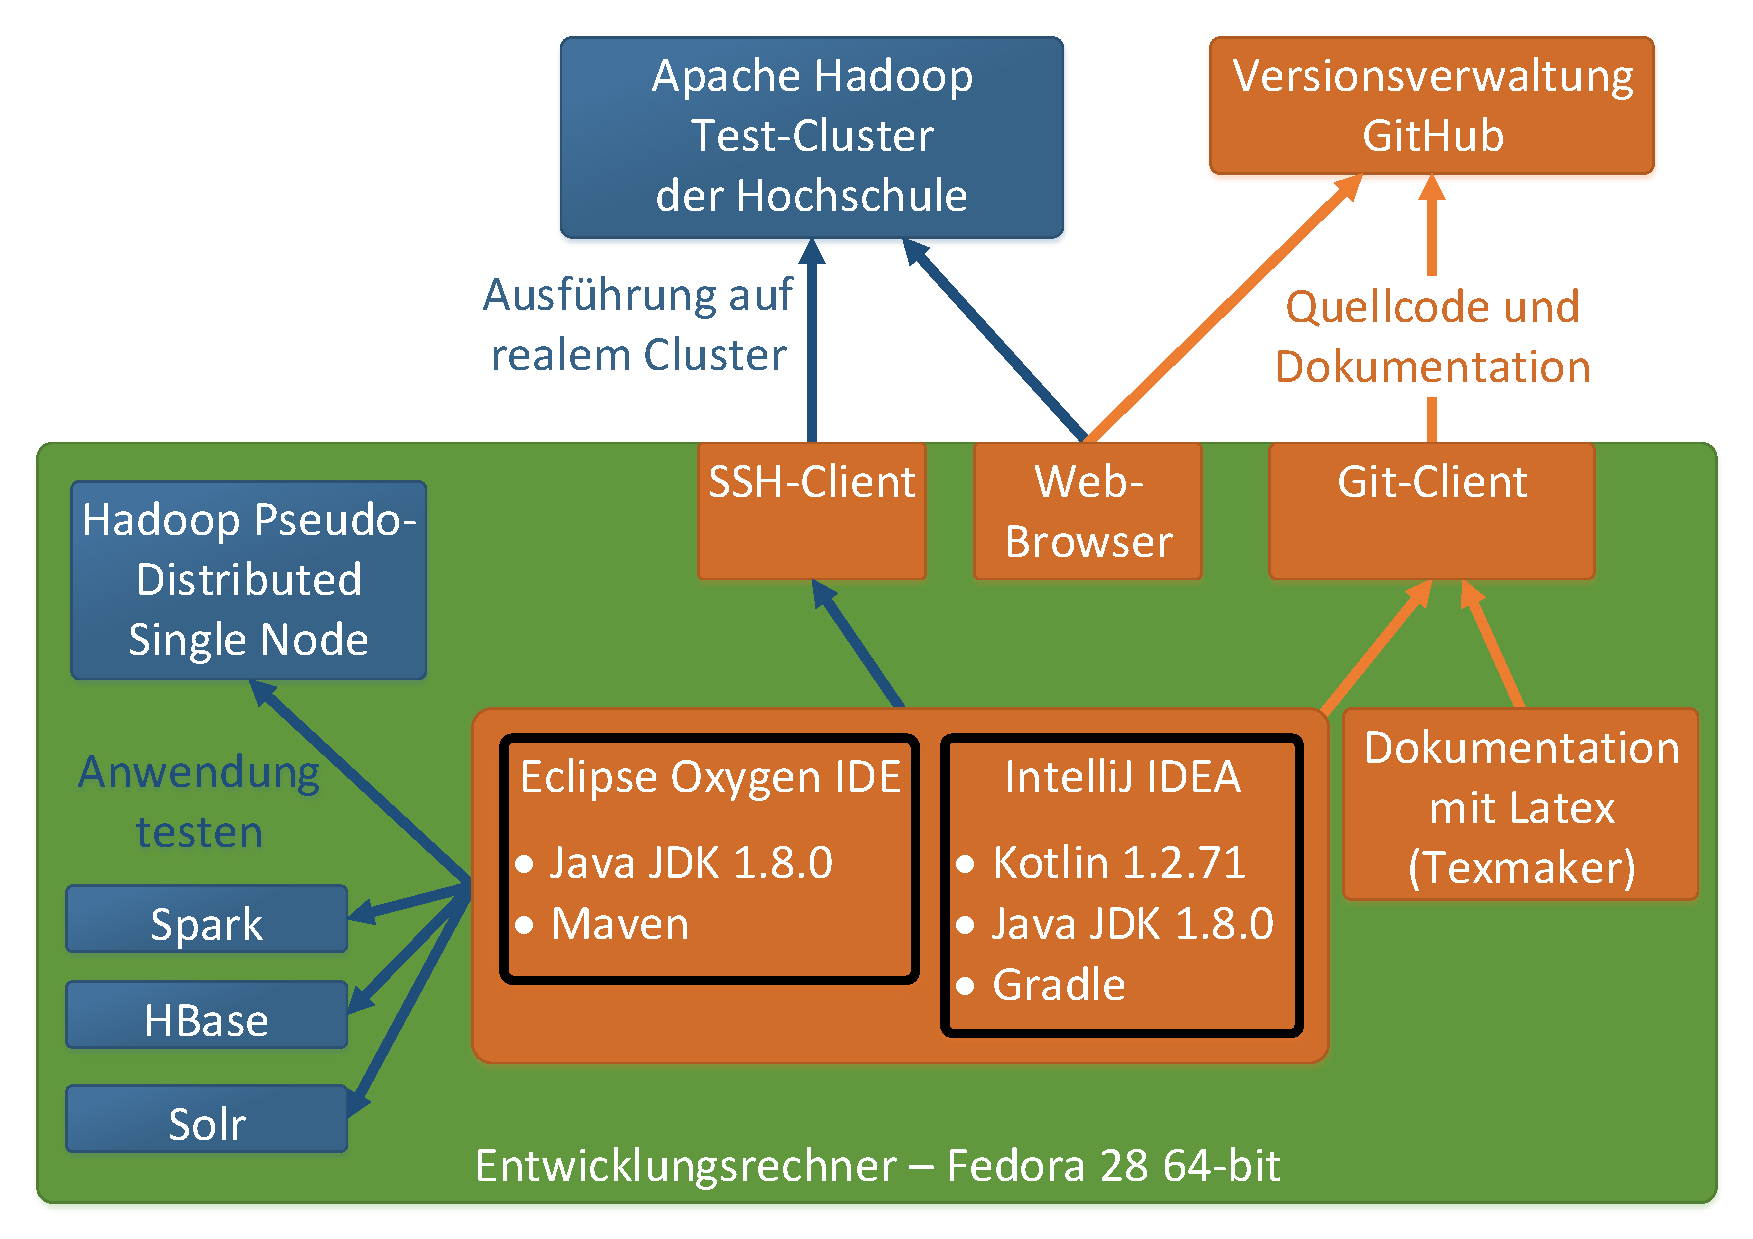
\includegraphics[width=\textwidth]{./resource/development_environment.pdf}
  \caption{Komponenten der Entwicklungsumgebung}
  \label{fig:development_environment}
\end{figure} 

\noindent
Zur Entwicklung der forensischen Analyseprogramme wird \textit{Eclipse Oxygen} genutzt. Die Anwendungen selbst werden in Java geschrieben.\footnote{Wobei auch Python oder Scala als Programmiersprache genutzt werden kann.} Zum Bauen der ausführbaren \gls{jar} wird \textit{Maven} verwendet. Mit Maven können weitere Java-Bibliotheken 
in eigenen Programmen auf einfache Weise wiederverwendet werden.\footnote{Diese können über ein zentrales Repository, dem sogenannten \textit{Maven Central Repository} aus dem Internet geladen werden (siehe Link\url{https://search.maven.org/}. Letzter Zugriff 26.8.2018).}\\

\noindent
Zusätzlich befindet sich die Entwicklungsumgebung \textit{IntelliJ IDEA} in der kostenlosen Cummunity Variante  auf dem Entwicklungsrechner. Mit der IntelliJ IDEA wird die Datenimport-Anwendung in \textit{Kotlin} entwickelt. Kotlin ist eine statisch typisierte Programmiersprache zur Anwendungsentwicklung auf verschiedenen Plattformen.\footnote{Siehe Link \url{https://kotlinlang.org/}. Letzter Zugriff: 24.8.2018.} Sie ist interoperabel mit Java. Die Anwendungen können in der \textit{Java Virtual Machine} (JVM) ausgeführt werden. Gegenüber Java bietet sie diverse Sprachkonstrukte zur Optimierung des Programmcodes an. Darüber hinaus können alle Bibliotheken aus dem Java-Umfeld auch in Kotlin genutzt werden. Zum Bauen der Kotlin-Anwendungen wird \textit{Gradle} genutzt, welches analog zu Maven Abhängigkeiten zu Drittbibliotheken und deren Versionen verwaltet.\footnote{Siehe auch Kapitel \ref{subsec:data_import_implementation} für weitere Informationen zur Datenimportanwendung.}\\


\noindent
Um die gebauten Java- und Kotlin-Programme schnell zu testen, können alle notwendigen Komponenten auch lokal auf dem Entwicklungsrechner gestartet werden. Hierzu gehört ein Hadoop-Knoten im sogenannten \textit{Pseudo-Distributed} Modus, eine lokale Spark-Instanz, eine HBase-Instanz und eine Solr-Instanz zur Datenindexierung.\footnote{Siehe Kapitel \ref{ch:theory_hadoop} für eine detaillierte Erklärung der Komponenten.}\\
Mithilfe dieser Komponenten können auch spezifische Konfigurationen getestet werden.\footnote{Hierfür muss der Entwicklungsrechner entsprechende Ressourcen bereitstellen. Es sollte mindestens eine Quad-Core-CPU, 16 GB Arbeitsspeicher und eine SSD zur Verfügung stehen, um performant arbeiten zu können.} \\
Letztendlich kommen die lokalen Instanzen schnell an ihre Grenzen, gerade wenn größere Datenmengen analysiert werden sollen. Daher werden spezifische Konfigurationen und fertiggestellte Analyseprogramme auch auf einem realen
Apache Hadoop-Cluster durchgeführt. Dort kann das Zusammenspiel zwischen den Komponenten nachvollzogen werden. Auch entsprechende Last-Tests sind nur auf dem Hadoop Test-Cluster möglich. Um mit dem Test-Cluster arbeiten zu können, wird ein SSH-Client benötigt. Zusätzliche gibt es auch eine Web-Oberfläche basierend auf Apache Ambari zur Konfiguration und Anzeige des aktuellen Systemzustandes.\\

\noindent
Alle selbst erstellten Anwendungsprogramme, Konfigurationsdateien und die Dokumentation dieser Thesis sollen als Open-Source Projekte in einem öffentlichen Repository zugänglich sein. Aus fachlicher Sicht ist es gerade in der Forensik sehr wichtig dem Nutzer die Möglichkeit zu geben, den Quellcode der Analyseprogramme einsehen zu können und notfalls auf spezielle Bedürfnisse anzupassen. Darüber hinaus kann die Datenverarbeitung transparent nachvollzogen werden.
Daher werden die einzelne Projekte mithilfe eines Git-Clients auf GitHub versioniert.\\
Nachfolgende Auflistung zeigt die Aufteilung der Projekte:
\begin{itemize}
\item Das Projekt \textit{foam-thesis}\footnote{Die Abkürzung \textit{foam} oder auch \textit{\acrshort{foam}} steht für \textit{\textbf{fo}rensische \textbf{A}nalyseplattfor\textbf{m}}} enthält die schriftliche Ausarbeitung der Thesis und den Quellcode als Latex-Projekt. Als Entwicklungsumgebung wird \textit{Texmaker} genutzt.\\
Über den Link \url{https://github.com/jobusam/foam-thesis} ist der aktuelle Stand der Arbeit jederzeit einsehbar.\footnote{Das kompilierte PDF-Dokument zum jeweiligen Stand wird im gleichen Projekt versioniert und ist unter dem Link \url{https://github.com/jobusam/foam-thesis/blob/master/main.pdf} verfügbar.}

\item Das Projekt \textit{foam-data-import} enthält den Quellcode zum Importieren von Asservaten in das Hadoop-Cluster. Unter \url{https://github.com/jobusam/foam-data-import} befindet sich die Kotlin-Anwendung, welche wiederum mit Gradle gebaut werden kann.

\item Das Projekt \textit{foam-processing-spark} enthält den Quellcode zur Auswertung mit Apache Spark\texttrademark\thinspace. Unter \url{https://github.com/jobusam/foam-processing-spark} befindet sich ein Maven-Projekt, welches wiederum die Java-Anwendung baut. Es werden auch entsprechende Skripte zum Starten von Spark-Anwendungen auf dem lokalen Rechner bereitgestellt. 

%TODO Installationsskripte zu HBase und Solr!
\item Das Projekt \textit{foam-storage-hadoop} enthält alle Konfigurationsdateien zum Aufsetzen eines Hadoop-Clusters auf einem einzelnem Knoten im \textit{Pseudo-Distributed Mode}.\footnote{Siehe Link \url{https://github.com/jobusam/foam-storage-hadoop/tree/master/hadoop.standalone.configuration}} Zusätzlich existieren Shell-Skripte zum Starten des Hadoop-Clusters auf einem einzelnen Knoten.\footnote{Siehe Link \url{https://github.com/jobusam/foam-storage-hadoop/tree/master/hadoop.standalone.setup}} Mithilfe der Skripte aus dem \textit{foam-processing-spark} Projekt können damit Spark-Anwendungen ausgeführt werden.
\end{itemize}

\noindent
Die Dokumentation der Thesis und alle erstellten Diagramme sind unter der \textit{\gls{ccbysa}} lizenziert. Der Quellcode der forensischen Analyseplattform und die erstellten Konfigurationen sind unter der Apache License 2.0 lizenziert. Es soll jeder Person möglich sein, den Quellcode und die Dokumentation anzuschauen und nach belieben ändern zu können.\\

\section{Testdatengenerierung}
\label{testdatacreation}
Für den Aufbau einer forensischen Analyseplattform sollen entsprechende Testdaten generiert werden. Hierzu werden zwei unterschiedliche Falldaten erzeugt. Der erste Fall ist ein kleines Datenträgerabbild mit knapp 10 GB Gesamtgröße. Dieses Image soll für lokale Tests genutzt werden, um die entwickelten Implementierungen zur Datenspeicherung und Verarbeitung schnell auf ihre Korrektheit prüfen zu können. Der Datenträger enthält eine Partitionen mit dem Ext4-Dateisystem. Darauf ist ein Ubuntu 16.04 LTS installiert. Zusätzlich sind auch noch einige Testdaten darauf gespeichert.\\

\noindent
Im zweiten Fall wird ein 155 GB großes Image erzeugt. Der Datenträger besteht wiederum aus einer Partition mit einem NTFS-Dateisystem. Darauf ist Windows 10 installiert. Zusätzlich sind größere Datensätze von Bildern und Musik aus dem Internet darauf gespeichert. Die Datensätze werden lizenzfrei als Trainingsdaten zum maschinellen Lernen angeboten. Dieses größere Datenträgerabbild kann zur Verarbeitung im Testcluster genutzt werden, um die Skalierbarkeit bei großen Datenmengen zu testen. Beide Datenträgerabbilder werden in Kapitel \ref{sec:performance_analysis} für Leistungstests verwendet. Hierzu befindet sich einige sehr große und auch viele kleine Dateien auf den Datenträgern, um möglichst realitätsnahe Testergebnisse zu erhalten.
\section{Apache Hadoop\textsuperscript{\textregistered} Framework}
\label{sec:theory_hadoop}
\noindent
Apache Hadoop ist ein etabliertes Java-Framework zur verteilten Speicherung und Verarbeitung von Daten. Durch die parallele Ausführung von Algorithmen eignet sich ein Hadoop-Cluster für rechenaufwendige Datenanalysen. Ein primäres Paradigma ist das Konzept der \textit{Datenlokalität}. Die auszuführenden Programme werden auf die Knoten verteilt, auf welchen auch die Daten liegen. Ressourcenintensive Datentransporte sollen weitgehend vermieden werden.\cite[S. 20 ff.]{big_data_praxis}\\ 
Das Framework ist für die Ausführung auf Standardhardware konzeptioniert. Es wird also keine verhältnismäßig teure Spezialhardware benötigt. Das Cluster besteht aus vielen einzelnen Knoten mit Standardhardware, welche im Verhältnis zu Spezialhardware günstiger und leicht ersetzbar ist. Der Ausfall einzelner Knoten ist die Regel und wird bei der Datenhaltung entsprechend berücksichtigt. \\

\noindent
Das Apache Hadoop\textsuperscript{\textregistered} selbst besteht aus mehreren Komponenten, welche spezifische Aufgaben übernehmen. Abbildung \ref{fig:hadoop_framework_structure} stellt eine grobe Skizzierung der Komponentenlandschaft von Apache Hadoop dar.\footnote{In der Abbildung \ref{fig:hadoop_framework_structure} werden Logos der einzelnen Apache Projekte verwendet. Diese sind Handelsmarken der \textit{Apache Source Foundation} (siehe \url{https://www.apache.org/}). In Kapitel \ref{sec:licencing_issues} im Anhang werden die Logos und deren Herkunft nochmals aufgelistet.}\\

\begin{figure}[ht]
  \centering
  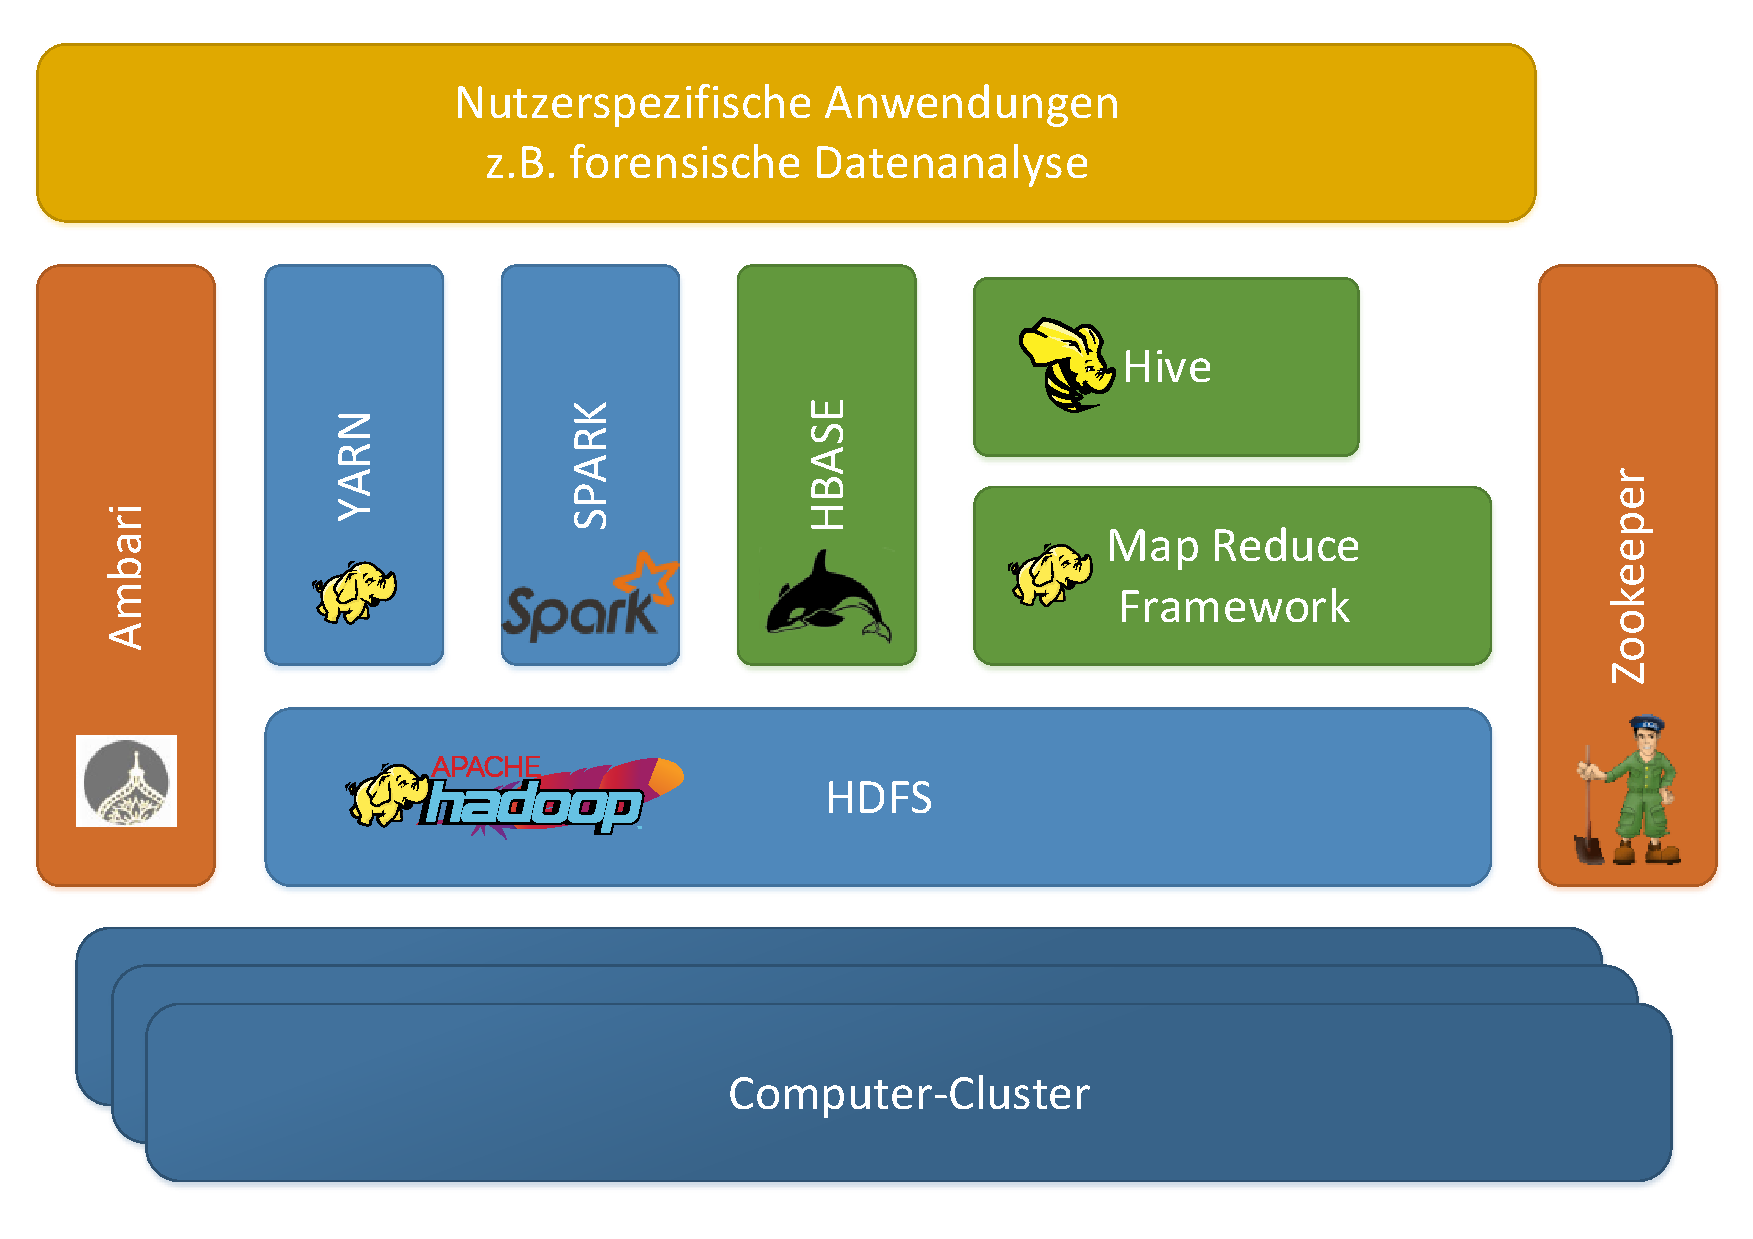
\includegraphics[width=\textwidth]{./resource/hadoop_framework_structure.pdf}
  \caption{Apache Hadoop Ökosystem (Vgl. \cite{big_data_praxis},\cite{expert_hadoop_admin}. Siehe Kapitel \ref{sec:licencing_issues})}
  \label{fig:hadoop_framework_structure}
\end{figure}

\noindent
Die Basis bildet das verteilte Dateisystem \textit{Hadoop Distributed File System (HDFS)}, welches die Daten redundant auf allen Knoten des Computer-Clusters speichert. Hierbei besteht das Computer-Cluster selbst aus mehreren Knoten, auf welchen vorzugsweise ein Linux-Betriebsystem, wie beispielsweise CentOS, arbeitet.\\
Der Ressourcenmanager \textit{YARN (Yet Another Resource Negotiator)} ist für die Verteilung und Bereitstellung von verfügbarer Rechenleistung verantwortlich.\\ 
Die dritte Komponente ist das \textit{Hadoop\textsuperscript{\textregistered} Map-Reduce Framework}. Hadoop Map-Reduce kann zur Datenverarbeitung genutzt werden. Hierbei werden Algorithmen parallel auf den Knoten prozessiert und die Ergebnisse im Anschluss zusammengetragen. Die einzelnen Zwischenergebnisse werden alle im HDFS abgelegt.\footnote{Sogenannte Map-Reduce Jobs bildeten in den Anfängen von Hadoop den primären Weg, Daten verteilt zu verarbeiten. Mittlerweile wurde diese Art der Datenverarbeitung in den Hintergrund verdrängt, da andere Projekte, wie beispielsweise Apache Spark, die Daten schneller verarbeiten können oder andere Ansätze zur Verarbeitung nutzen. Dies ist beispielsweise auch der Grund, weshalb Hadoop Map-Reduce in dieser Masterthesis nicht explizit verwendet wird.} \\

\noindent
Das verteilte Dateisystem HDFS und der Ressourcenmanager YARN bilden den Kern des Hadoop-Clusters. Darauf aufbauend können andere Komponenten die Daten verarbeiten oder spezielle Aufgaben durchführen.\\
So wird beispielsweise in dieser Thesis \textit{Apache Spark\texttrademark\thinspace} bei der Prozessierung und Analyse der Daten genutzt. Der Vorteil von Apache Spark ist eine performante Datenverarbeitung, da einerseits die Daten verteilt verarbeitet werden und andererseits Zwischenergebnisse und temporäre Daten im Arbeitsspeicher der einzelnen Rechenknoten gehalten werden.\footnote{Durch das In-Memory Computing ist Apache Spark deutlich schneller als das bereits vorgestellte Hadoop Map-Reduce.}\\
Desweiteren bietet \textit{Apache Hive\texttrademark\thinspace} eine Möglichkeit Dateien im HDFS mithilfe einer SQL ähnlichen Syntax\footnote{Dem sogenannten HiveQL.} abzufragen. Hierbei nutzt die Komponente wiederum das Map-Reduce Framework von Hadoop. Apache Hive ist jedoch keine reine Datenbank, sondern arbeitet auf den Dateien im HDFS.\\
\textit{Apache HBASE\textsuperscript{\textregistered}} hingegen ist eine spaltenorientierte Key-Value Datenbank. Sie wurde eigens für Apache Hadoop implementiert, 
um große Datenmengen performant zu speichern.\\

\noindent
Das Hadoop-Ökosystem als Ganzes muss auch konfiguriert und überwacht werden. Um die Verfügbarkeit einzelner Instanzen zu gewährleisten und gegebenenfalls redundante Verarbeitungswege anzubieten, wird \textit{Apache ZooKeeper\texttrademark\thinspace} genutzt. Mit ZooKeeper ist es auch möglich Konfigurationen und Änderungen im Cluster zu verteilen. Zum eigentlichen konfigurieren und überwachen des Hadoop-Clusters wird \textit{Apache Ambari\texttrademark\thinspace} genutzt.\\

\noindent
Zusätzlich existieren weitere Projekte im Hadoop-Ökosystem, welche für die forensische Analyseplattform von Verwendung sein können.
Hierzu gehören:
\begin{itemize}
\item \textit{Apache Livy} zur Ausführung von Apache Spark Anwendung über eine REST-Schnittstelle.\footnote{\textit{Representational State Transfer (REST)} bezeichnet ein Programmierparadigma in verteilten Systemen. Hierbei werden Ressourcen über HTTP angefordert, gespeichert und verarbeitet.}
\item \textit{Apache NiFi} ermöglicht das Aufbereiten von Daten und organisiert Datenimporte.
\item \textit{Apache UIMA\texttrademark\thinspace} zur Analyse von unstrukturierten Daten, wie beispielsweise Texte und Mediadateien. \textbf{TODO: Kann UIMA überhaupt in Hadoop eingesetzt werden.}
\item \textit{Apache Accumulo\textsuperscript{\textregistered}} als Alternative zu Apache HBASE?
\end{itemize} 

\noindent
Prinzipiell sind viele Komponenten unabhängig voneinander. So kann ein HDFS ausschließlich zur Datenhaltung aufgebaut werden, ohne eine Komponente zur Datenverarbeitung verwenden zu müssen. Umgekehrt lassen sich Komponenten zur Datenverarbeitung, wie Apache Spark, auch ohne das HDFS und YARN nutzen und könnten damit auch in andere Umgebungen integriert werden. Die einzelnen Komponenten entfalten jedoch gerade durch die Kombination miteinander ihre Potential zur performanten Datenanalyse.\\

\noindent
Es gibt einige Unternehmen, die sich speziell daruf spezialisiert haben dieses Apache Hadoop Ökosystem und weiter noch nicht erwähnte Komponenten zu einzelnen Analyseplattformen zusammenzufassen. Sie bieten hierfür entsprechender kostenpflichtiger Support, wobei diese Plattformen im reinen Betriebe kostenfrei sind. So wird im Praxisteil der Masterthesis beispielsweise die \textit{Hortonworks Data Platform (HDP)} des Unternehmes \textit{Hortonworks} genutzt.


\section{Apache Hadoop HDFS}
\label{sec:theory_hdfs}
Das Hadoop Distributed Filesystem (HDFS) ist ein verteiltes Dateisystem, welches die Grundlage zu Speicherung von Daten im Hadoop-Ökosystem bietet. Nachfolgende Zwecke soll es erfüllen.\\
Es soll ausfallsicher sein. In der Standardkonfiguration wird jede Datei dreifach auf unterschiedlichen physikalischen Knoten gespeichert. Damit kann selbt bei einem Ausfall von zwei Knoten immer noch auf die Datei zugegriffen werden. Darüber hinaus verteilt das HDFS die Dateien automatisch und regeneriert sich selbst nach Ausfällen von Knoten. In großen Computer-Clustern mit mehreren hunderten Knoten ist ein Ausfall eines Knoten kein Sonderfall sondern die Regel. Daher muss sich das HDFS selbst heilen können, um auch ohne manuelle Administration weiter verfügbar zu sein.\\
Das HDFS (und auch Hadoop im allgemeinen) soll horizontal skalierbar sein. Wird mehr Speicher benötigt, sollen einfach noch Knoten hinzugefügt werden können.\\
Das HDFS ist auf hohen Datendurchsatz und die Speicherung großer Datenmengen ausgelegt.
So können einzelne Dateien mehrere Gigabyte bis hin zu Terrabyte groß seind und es können mehrere Millionen Dateien im HDFS gespeichert werden. Die Optimierung auf einen möglichst hohen Datendurchsatz geht mit einer schlechteren Reaktionszeit im Vergleich zu herkömlichen Dateisystemen einher.\\
Das Prinzip \textit{Write-once-Read-many} wird im HDFS implementiert. Wenn Daten einmal geschrieben wurden, dann werden sie normalerweise nicht mehr geändert. Dies ermöglicht ein einfacheres Koherenzmodell. Dies fördert den Lesedurchsatz indem die Unterstützung der Modifikation von Daten stark eingechränkt wird. Ein wahlfreies Schreiben in eine existierende Datei wird beispielsweise nicht unterstützt. Änderungen an Daten, welche von Algorithmen vorgenommen werden, resultieren in neuen Datensätzen.\\
Darüber hinaus gilt das Prinzip der Datenlokalität. Algorithmen werden dort ausgeführt, wo die Daten liegen, um das Verschieben von Daten über das Netzwerk zu vermeiden.\cite{hdfs_architecture}\\

\noindent
Der Aufbau eines HDFS bildet eine Master-Slave Architektur aus \textit{NameNodes} und \textit{DateNodes}. Der NameNode is einmalig im verteilten System vorhanden und enthält alle Metainformationen zu den Dateien. Eine Datei selbst wird in ein oder mehrere Blöcke aufgeteilt und auf mehreren DateNodes gespeichert. Der NameNode organisiert diese Speicherung und bestimmt, wo welche Daten persistiert werden. Über den NameNode selbst fließen aber keine Rohdaten von Dateiinhalten. Auf Dateisystemebene ist das HDFS wie gängige Dateisystem hierarchisch organisiert. Jede Datei wird über einen absoluten Pfad eindeutig bestimmt und erhält entsprechende Metadaten, wie Dateirechte und Zeitstempel.  \\

\noindent
Abbildung \ref{fig:hdfs_cluster_architecture} verdeutlicht die Struktur im HDFS. Angenommen es soll die Datei \path{/home/foo.txt} gespeichert werden. Dies kann mit dem Terminalprogramm \textit{hdfs} durchgeführt. Das Programm selbst ist hier der HDFS-Client und hat Zugang zum Hadoop-Cluster. Der HDFS-Client speichert zuerst die Metadaten der Datei auf dem Name Node. Der Name Node bekommt die Größe der Datei auch mit und entscheidet dann, in viele Blöcke sie unterteilt werden soll. Darauf hin ermittelt für jeden einzelnen Block, auf welchen Date Nodes dieser Block gespeichert werden soll. Diese Blockaufteilung und die Zuordnung zuden Date Nodes werden an den HDFS-Client zurückgeschickt. Dieser übermittelt die Blöcke an einen der Data Nodes. Sobald der erste Data Node einen Block hat, sorgt er dafür die Blöcke an die anderen Data Nodes weiterzuleiten. Die Data Nodes selbst stehen auch in Kontakt zum Name Node und reporten ihren Zustand und die momentan gespeicherten Blöcke. Der Name Node bekommt darüber auch mit, wenn ein Data Node ausfällt.

\begin{figure}[ht]
  \centering
  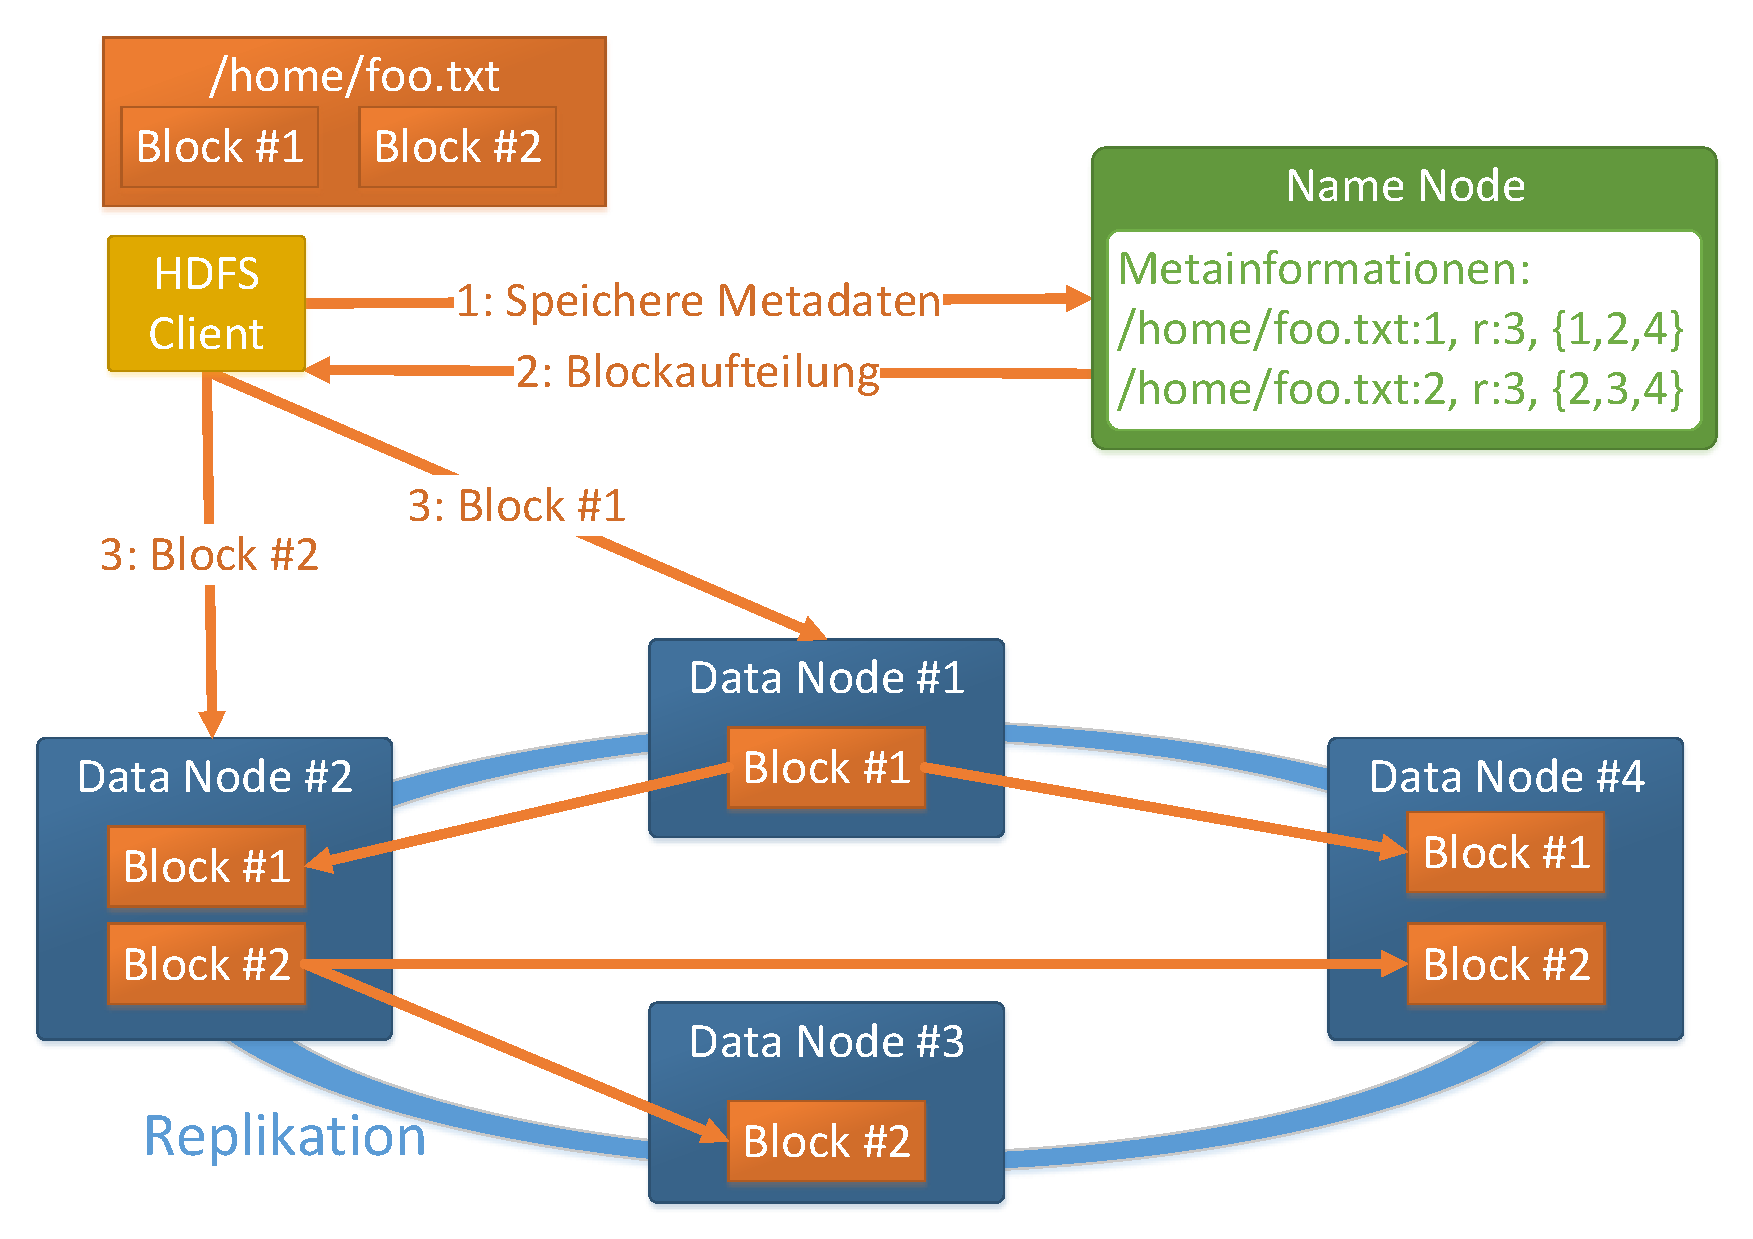
\includegraphics[width=\textwidth]{./resource/hdfs_cluster_architecture.pdf}
  \caption{HDFS - Datenspeicherung im Verbund (Vgl. \cite{hdfs_architecture},\cite{expert_hadoop_admin})}
  \label{fig:hdfs_cluster_architecture}
\end{figure}

\noindent
Ein Block hat in der Standardkonfiguration 128 MB. Er kann aber auch bis zu 512 MB Größe konfiguriert werden. Dies wirft die Frage auf, ob das HDFS gerade für sehr kleine Dateien, wie sie bei der Analyse von Datenträgern auch vorkommen, nicht zu viel Speicher verschwendet. \\
Hierbei wird der gleiche Block immer in unterschiedlichen Data Nodes angelegt. Es ist nicht erlaubt den gleichen Block mehrmals im gleichen Data Node zu replizieren. Daher ist die Anzahl der Replikationen auch kleiner gleich der Anzahl Data Nodes im System.

\noindent
Wichtig hierbei ist auch, dass im Produktivsystem auf jedem physikalischen Knoten auch nur ein DataNode oder ein NameNode läuft. Denn würden beispielsweise mehrere DateNodes auf dem gleichen physikalischen Knoten laufen, so wäre bei einem Ausfall nicht mir garantiert, dass die Dateiinhalte auch noch auf mindestens zweie anderen Knoten laufen. Denn der Replikationsmechanismus im HDFS kann nicht erkennen, ob jeder Knoten physikalisch unabhängig arbeitet. Allerdings hat Hadoop eine sogenannte \textit{Rack-Awareness}. So ist es möglich zu bestimmen, welche physikalischen Server in einem gemeinsamen Rack laufen. Abhängig davon, versucht das HDFS die Daten teilweise im selben Rack redundant zu speichern aber auch einige Replikationen außerhalb des Racks anzulegen. So kann auch der Ausfall eines Racks im Notfall kompensiert werden.\\
In Testumgebungen ist aber schön möglich sogar NameNode und mehrere DateNodes auf einem Knoten laufen zu lassen. Allerdings greifen die Mechanismen für eine Toleranz gegenüber Hardwareausfällen dann nicht mehr.\\

\noindent
Wie oben ersichtlich, ist der Name Node die Schlüsselstelle im HDFS-Cluster. Dieser bildet einen \textit{Single Point of Failure}. Denn bei einem Ausfall wäre das HDFS nicht mehr einsatzbereit. Es existiert ein sogenannter \textit{Secondary Name Node}. Dieser erhält die Metainformationen und erstellt daraus regelmäßig Checkpoints. Der Name Node hält die Metainformationen im Arbeitsspeicher. Es existiert aber auch eine Datei \textit{FsImage} und ein \textit{EditLog}, welche persistent auf der Festplatte gespeichert sind. Das FsImage selbst beschreibt einen Zustand der Dateisystemmetainformationen zu einem gewissen Zeitpunkt. Im EditLog befinden sich alle Änderungen seit dem letzten Checkpoint bis zum aktuellen Zeitpunkt. Der Secondary Name Node erstellt aus dem FsImage und dem EditLog regelmäßig neue Checkpoints, die dann der produktive Name Node bei einem möglichen Neustart wiederverwenden kann. Der \textit{Secondary Name Node} unterstützt also den (First) Name Node, er kann ihn aber nicht ersetzen.\\
Daher ist es möglich auch einen sogenannten \textit{Standby Name Node} zu konfigurieren. Dieser kann einspringen, sobald der erste Name Node ausgefallen ist. Allerdings muss dieser extra konfiguriert werden. Dafür kann aber dann der Secondary Name Node deaktiviert werden.\cite[S. 88]{expert_hadoop_admin}\textbf{ TODO: prüfen ob das wirklich stimmt!}\\

\noindent
Das HDFS selbst kann über mehrere Wege genutzt werden. Es gibt eine Kommandozeilenschnittstelle, die sogenannte \textit{FS Shell}. Es ist möglich über eine Java oder C++ - Schnittstelle Datenzugriff zu erhalten. Oder das Dateissystem kann über eine REST-Schnittstelle via HTTP(S) genutzt werden. Auch das Mounten als \textit{Network File System (NFS)} ist möglich?

\section{Apache Hadoop YARN}
\label{sec:theory_yarn}
YARN ist ein Ressourcenmanager, welcher die verfügbaren Ressourcen innerhalb des Hadoop Clusters organisiert und die Ausführungsreihenfolge von Jobs plant und überwacht. Es gibt einen \textit{Resource Manager}, welcher nur die Ressourcen verwaltet. Auf jedem Knoten, welcher auch Datenverarbeitungen durchführt, ist ein \textit{Node Manager} aktiv. Zuletzt gibt es noch einen \textit{Application Manager} für jeden einzelnen Job, der ausgeführt werden soll. Der Application Manager kontrolliert die Ausführung des Jobs.\\
Abbildung \ref{fig:yarn_cluster_architecture} zeigt die Komponenten von YARN im Cluster.\\

\begin{figure}[ht]
  \centering
  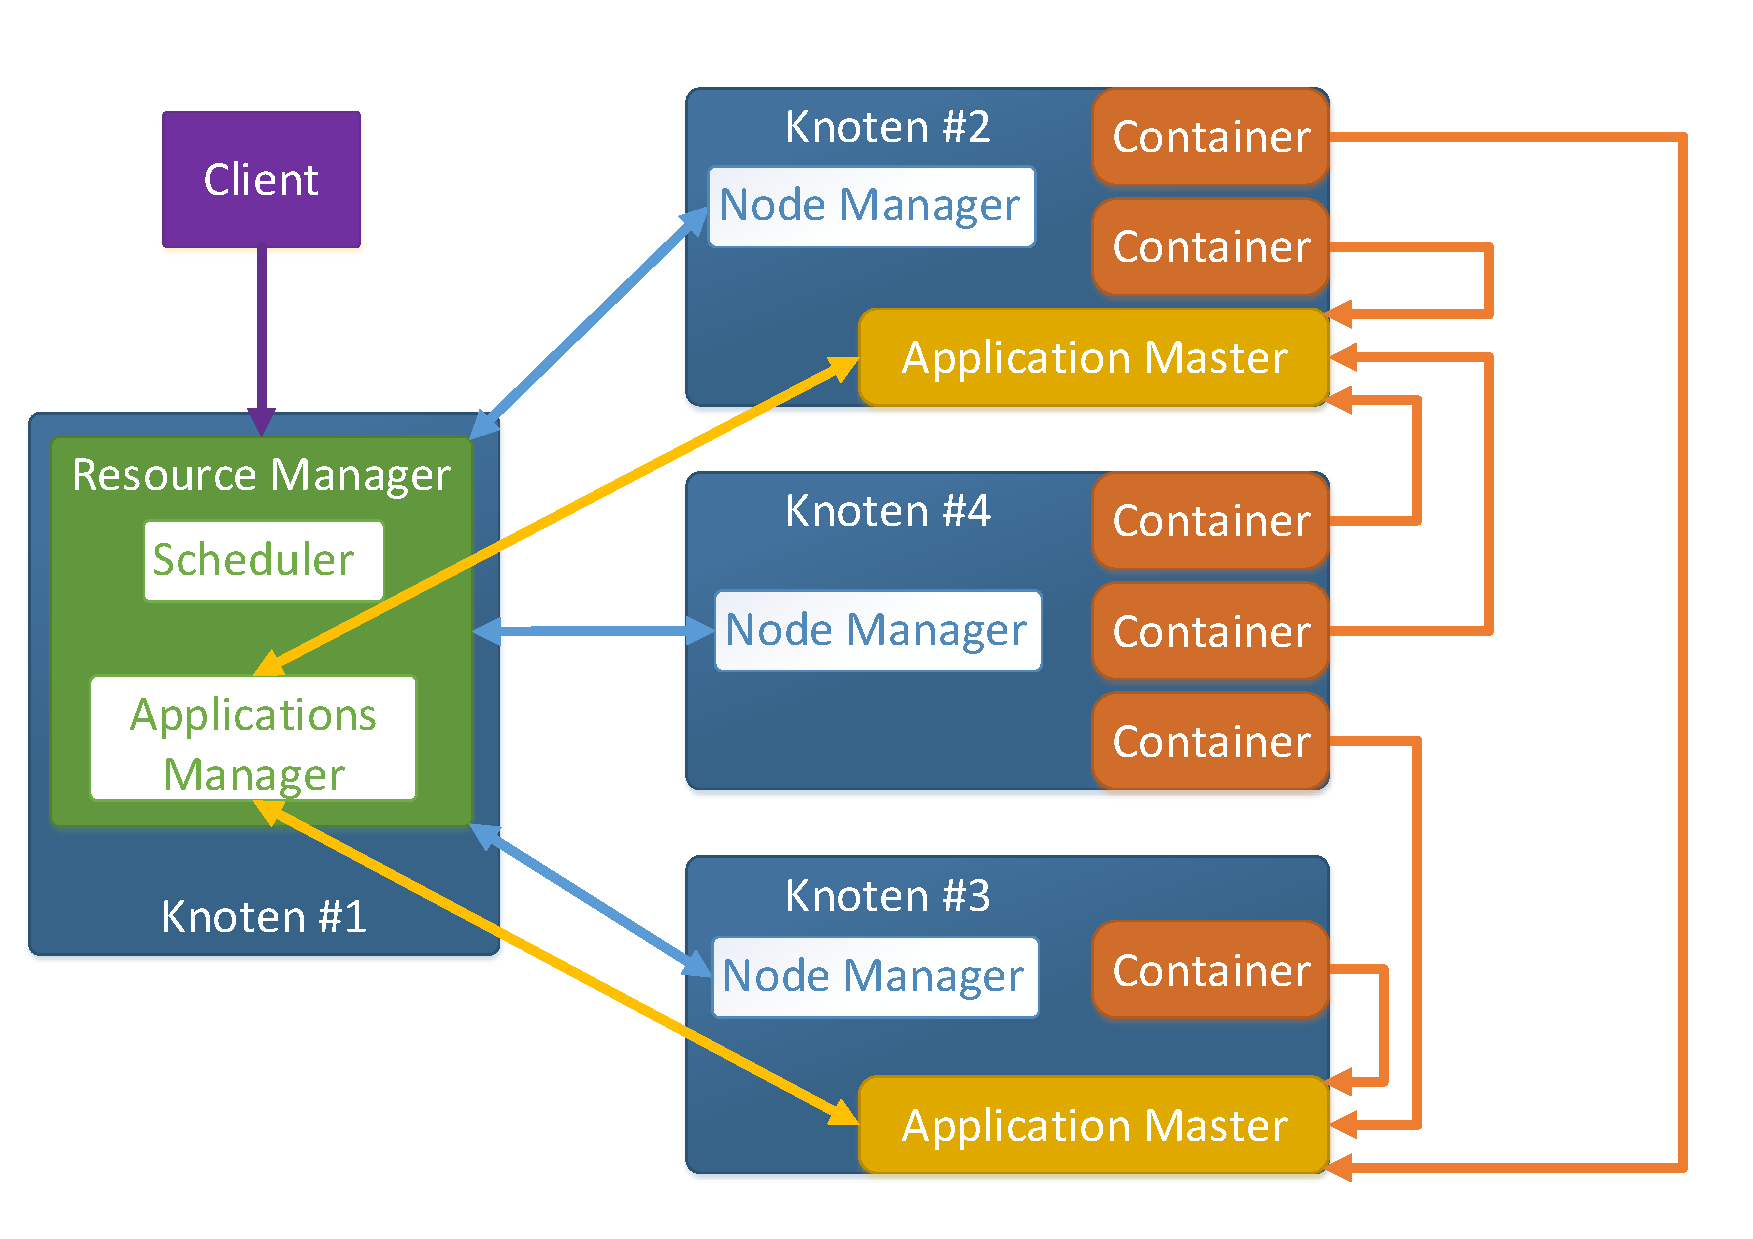
\includegraphics[width=\textwidth]{./resource/yarn_cluster_architecture.pdf}
  \caption{Ressourcenverteilung mit YARN (Vgl. \cite{yarn_architecture},\cite{expert_hadoop_admin})}
  \label{fig:yarn_cluster_architecture}
\end{figure}

\noindent
Ein Job oder eine Anwendung besteht aus mehreren Tasks. Diese Tasks können parallel in mehreren sogenannten Container ausgeführt werden. Ein Container ist eine abstrakte parallele Verarbeitungseinheit, welche bestimmte CPU- und Speicher-Ressourcen enthält. Es können mehrere dieser Container auf einem Knoten innerhalb des Clusters ausgeführt werden. Beispielsweise werden bei einem Knoten mit einer Quad-Core CPU und Hyperthreading (mit insgesamt 8 ausführbaren Threads) bis zu 8 Container erstellt. Bei 32 GB Arbeitsspeicher könnten dann jedem Container 4 GB zugeteilt werden.\footnote{In der Praxis ist es meistens weniger, da entsprechende Ressourcen für das darunter liegende Betriebssystem und YARN selbst reserviert werden.}\\
Derzeit werden für den Container die Anzahl der CPU-Cores (Ausführbare CPU-Threads) und die Größe des nutzbaren Arbeitsspeichers definiert.\cite[S. 48 ff.]{expert_hadoop_admin}\\

\noindent
Wenn nun eine Anwendung über YARN im Cluster ausgeführt werden, soll dann sendet ein Client eine Anfrage an den Resourcen Manager. 
Für jeden auszuführenden Job erstellt der Resource Manager den ersten Container. In diesem Container wird dann der Application Manager gestartet, welcher sich dann im weiteren Verlauf um die Ausführung des Jobs kümmert. Der Resource Manager selbst kennt die Anwendung nicht, noch weiß er wie diese ausgeführt werden. 
Er ist nur dafür zuständig Resourcen zu verteilen.\\ 
Der Application Master hingegen ist sehr spezifisch. Wird zum Beispiel eine Apache Spark Anwendung mit YARN ausgeführt, so ist der Application Master der sogenannte \textit{Spark App Master}. Nachdem nun der Application Master mit im ersten erzeugten Container gestartet wurde, kann dieser wiederum neue Ressourcen beim Resource Manager anfordern. An dieser Stelle zeigt sich der Vorteil von YARN in Kombination mit dem HDFS. Denn bei der Anforderung von Ressourcen gibt der Application Manager an, wieviele Container (inklusive Arbeitsspeicher und CPU) er benötigt. Zusätzlich übermittelt er die Dateiblöcke, welche er aus dem HDFS braucht und an welchen Knoten er welche Container gerne starten würde. So würde der Application Manager 1 auf dem Knoten 2 (siehe Abbildung \ref{fig:yarn_cluster_architecture}) einen Container auf dem Knoten 2 und zwei Container auf dem Knoten 4 mit beispielsweise 1 GB Arbeitsspeicher und 1 Core anfordern. Denn der Application Master weiß, dass dort die benötigten Datenblöcke im HDFS gespeichert sind. Hierbei ist es wichtig zu verstehen, dass die Knoten aus Abbildung \ref{fig:yarn_cluster_architecture} den Data Nodes aus Abbildung \ref{fig:hdfs_cluster_architecture} entsprechen.\footnote{Wobei ein physikalischer Knoten, auf welchem ein Data Node läuft nicht zwingend auch für die Datenverarbeitung mit YARN verwendet werden muss. Beziehend auf das Paradigma der Datenlokalität ist dies aber der Normalfall, dass ein Knoten, welcher Daten persistiert, auch Daten verarbeiten wird.}\\

\noindent
Der Application Master erhält dann die Zustimmung vom Resoure Manager, nachdem der Scheduler die geforderten Resourcen entsprechend eingeteilt hat. Darauf fordert der Application Manager den Node Manager auf den jeweiligen Knoten auf, entsprechende Container zu erstellen.\\
Die einzelnen Node Manager stehen in Kontakt zum Resource Manager und reporten ihm den aktuellen Status des Knoten und dessen Auslastung. \\
Nach der Ausführung der einzelnen Tasks innerhalb der Container und dem Abschluss des Jobs, schickt der Application Manager die Ergebnisse direkt zurück zum Client.\footnote{Hierbei werden die fachlichen Ergebnisse, meistens als Datei im HDFS gespeichert.}. Danach meldet er sich beim Resource Manager ab. Zuletzt kümmert sich der Resource Manager dann über das Freigeben von allokierten Resourcen.\\

\noindent
Ähnlich wie beim Prozessschedulung in ein herkömmlichen Betriebssystem, gibt es auch für YARN unterschiedlicher Algorithmen, die festlegen, in welcher Reihenfolge und Zeitdauer die einzelnen Jobs ausgeführt werden. Bekannte Scheduler sind der \textit{Fair Scheduler} und der \textit{Capacity Scheduler}. Abhängig von der genutzten Plattform/Distribution einzelner Hersteller ist für YARN ein anderer Scheduler konfiguriert. In etlichen Fällen wird der Capacity Scheduler als Standard konfiguriert, da dieser versucht alle Knoten möglichst effizient auszusteuern um den höchstmöglichen Datendurchsatz durch erreichen. Der Fair-Scheduler prüft hingegen, dass jedem Job die gleichen Ressourcen zugeteilt werden, um möglichst alle Jobs parallel bedienen zu können.\textbf{TODO: Scheduling prüfen!}

\noindent
In großen Clustern wird die Prozessierung in mehrere Sub-Cluster mit eigenen Resource Managern aufgeteilt. Diese Struktur wird in der Literatur als \textit{Federaded YARN} beschrieben und soll die Skalierbarkeit von YARN in großen Clustern ermöglichen.

\section{Apache Spark}
\label{sec:theory_spark}

\textit{Apache Spark\texttrademark\thinspace} ist ein Projekt zur verteilten Prozessierung von großen Datenmengen. Mit Apache Spark können verschieden Algorithmen und Verarbeitungsschritte über eine einheitliche Programmierschnittstelle auf gespeicherte Daten  angewendet werden. Spark selbst kümmert sich um die Verteilung, Ausführung und Überwachung der Applikationen zur Datenverarbeitung.\cite[S. 2]{learning_spark}\\
Apache Spark ist mittlerweile schon fast der Standard, wenn es im Hadoop-Umfeld um die Datenverarbeitung geht. Es löst damit auch das ursprünglich verwendete MapReduce-Framework von Hadoop ab, denn Spark
bietet einen enormen Geschwindigkeitsvorteil gegenüber dem MapReduce-Framework. Dies lässt auf einer intelligenten Ausführung einzelner Verarbeitungsschritte und diversen Optimierungen zurückführen.\cite[S. 148 ff.]{expert_hadoop_admin}\\

\noindent
Ein anderer Aspekt sind auch die vielseitigen Einsatzzwecke von Spark. So wird die klassische Datenverarbeitung von statischen Datenmengen\footnote{In diesem Kontext ist das einfache Ausführen einer Anwendung auf eine bereits existierende Datenmenge gemeint, welches am Ende an definiertes Ergebnis liefert.} unterstützt auch die Verarbeitung von dynamischen Datenmengen (Streaming-Data) \footnote{Bei der Datenverarbeitung von Streaming-Data wächst die zu verarbeitende Datenmenge dynamisch and und die ausgeführte Anwendung verarbeitet die neu hinzugekommenen Daten. Ein Beispiel wäre das Filtern von Tweets auf Twitter nach bestimmten Merkmalen, wobei auch neu hinzukommende Tweets bearbeitet werden und nicht nur die Tweets, welche beim Ausführungszeitpunkt der Anwendung bereits existierten.}. Auch die Prozessierung von Graphen-Strukturen und das maschinelle Lernen werden unterstützt.\cite[S. 152]{expert_hadoop_admin}
Darüber hinaus steht es dem Anwender frei, ob er seine Applikationen in Scala, Python oder Java schreibt. Gerade bei den Interpreter-Sprachen Scala und Python gibt es sogar ein Spark-Shell zur interaktiven Datenverarbeitung und Analyse. Diese Vielseitigkeit macht sich auch in unzähligen Projekten und Programm-Bibliotheken bemerkbar, welche rund um Apache Spark entwickelt werden.\\ 
Es existieren diverse Anbindungen zu Datenspeichern, die sogenannten \textit{Spark-Connectoren}. Damit können beliebige Datenspeicher als Datenquelle verwendet werden.
Beispielsweise können Daten aus dem HDFS geladen werden, aber auch direkt aus Datenbanken wie HBASE, Cassandra, Neo4j oder Elasticsearch, welches zur Datenindexierung genutzt wird.  \\

\noindent
Abbildung \ref{fig:spark_cluster_architecture} zeigt die Ausführung einer Spark-Applikation innerhalb eines Hadoop-Clusters mit YARN und skizziert den physikalischen Kontext im Cluster. Dieser Aufbau beschreibt im Kontext der Thesis den primären Anwendungsfall zur Datenverarbeitung.\\ 
Apache Spark könnte auch vollständig unabhängig von dem Hadoop-Framework in einem eigenen Spark-Cluster ausgeführt werden und bietet dafür auch einen eigenen Ressourcenmanager. Allerdings wird innerhalb des Hadoop-Umfelds die Spark-Ausführung mit dem bereits erwähnten Ressourcenmanager YARN durchgeführt (siehe Kapitel \ref{sec:theory_yarn}). Dies hat auch
den Vorteil, dass YARN die Ressourcen auf den einzelnen Knoten besser verwalten kann. Denn wenn der Spark-Ressourcenmanager parallel zu YARN auf den gleichen Knoten genutzt werden würde, so könnte dies zu Ressourcen-Engpässen führen. Denn die Ressourcenmanager würden nicht miteinander kommunizieren und die Last der ausgeführten Anwendungen im Cluster könnte nicht gleichmäßig verteilt werden. Aus diesem Grund ist es ratsam YARN auch die Ausführung von Spark-Anwendungen im Cluster zu überlassen.\\

\begin{figure}[ht]
  \centering
  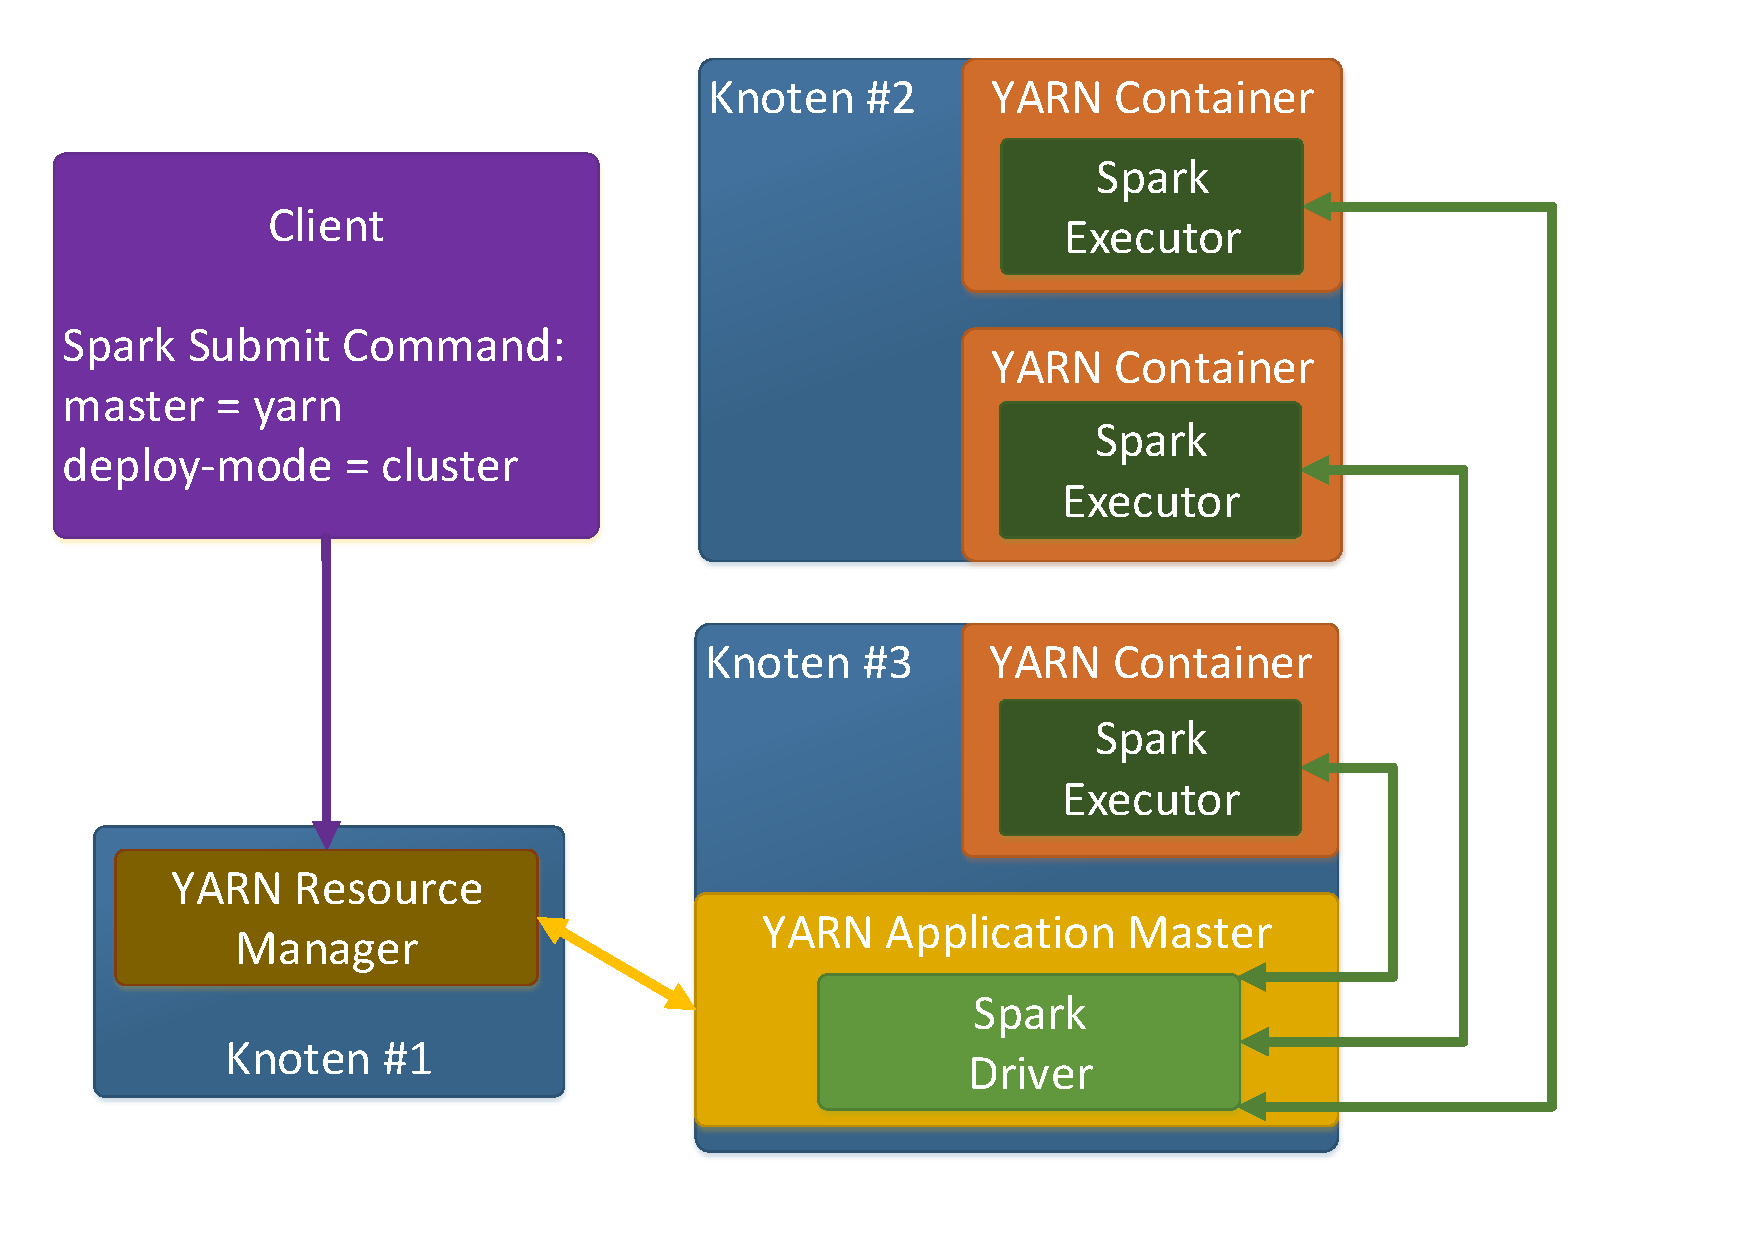
\includegraphics[width=\textwidth]{./resource/spark_cluster_architecture.pdf}
  \caption{Spark Datenverarbeitung im Cluster}
  \label{fig:spark_cluster_architecture}
\end{figure}

\noindent
Wie in Abbildung \ref{fig:spark_cluster_architecture} ersichtlich, wird die Ausführung einer Spark-Anwendung über den YARN-Ressourcenmanager gestartet. Es gibt hierbei unterschiedliche Wege, wie eine Spark-Anwendung ausgeführt werden kann. Im konkreten Fall wird das \textit{Spark-Submit} Kommando genutzt. Letztlich handelt es sich hierbei um einen Konsolenbefehl, welcher die Anwendung\footnote{Beispielsweise ist dies bei einer Spark-Anwendung in Java ein herkömmliches \textit{Java Archiv} im \textit{JAR}-Dateiformat.} selbst entgegennimmt und über diverse Parameter konfiguriert werden kann. So kann unter anderem der Master und Deploy Mode so konfiguriert werden, dass YARN die Ressourcen der Applikation verwaltet. Wie in Abbildung \ref{fig:yarn_cluster_architecture} (siehe Kapitel \ref{sec:theory_yarn}) bereits beschrieben, wird bei YARN ein ein Application Master erstellt, welcher wiederum diverse Ausführungscontainer auf den einzelnen Knoten anfordert und dieser überwacht. Bei der Ausfürung einer Spark-Anwendung werden diese Komponenten wiederverwendet und kapseln letztlich die falchlichen Komponenten von Spark.\\
So gibt es bei Spark einen sogenannten \textit{Driver}, welcher im Yarn Application Master läuft und wiederum die sogenannten \textit{Executor} aussteuert. Diese laufen wiederum gekapselt in einzelnen YARN Containern auf den Knoten. Ein Spark Executor entspricht aus Betriebssystemsicht eines Knotens im Cluster der Ausführung einer Java Virtual Machine (JVM) in einem eigenständigen Prozess. Aufgrund der Kapselung durch YARN können die einzelnen JVM-Prozesse überwacht werden und zur Not auch beendet werden, falls sie zu viel Ressourcen auf den Knoten anfordern.\\

\noindent
Hierzu muss Spark und YARN aber entsprechend konfiguriert werden, damit die Anwendungen auch korrekt im Cluster skaliert werden können. Nachfolgende Beispiel zeigt hier Konfigurationsmöglichkeiten.\\
Bei YARN und auch Spark beziehen sich die Ressourcen auf die Anzahl der genutzten CPU-Cores\footnote{Hierbei geht es um die virtuell verfügbaren CPU-Cores. So verfügt beispielsweise eine Intel CPU mit vier physikalischen Cores und Hyperthreading über insgesamt 8 virtuelle Cores zur parallelen Ausführung von Prozessen.} und die Größe des genutzten Arbeitsspeichers.\\

\noindent
\textbf{TODO}: Configurations Parameter in Cluster!\\

\noindent
Gerade wenn YARN einzelne Application-Container stoppt, weil sie zu viel Arbeitsspeicher benötigen deutet dies auf eine falsche Konfiguration oder falsche Programmierung der Spark-Anwendungen hin. Oftmals wird gerne der nutzbare Arbeitsspeicher pro Executor höher konfiguriert. Diese ist in den meisten Fällen jedoch der falsche Ansatz, da hierdurch kritische Probleme in der Programmlogik der Anwendung oftmals  nur kaschiert werden.\\ Daher ist es auf jeden Fall auch sinnvoll bei der Anwendungsentwicklung relativ kleine Cluster mit geringen Ressourcen zu nutzen, denn auch dort müssen die Anwendungen fehlerfrei ausführbar sein. Lediglich die Ausführungsgeschwindigkeit sollte sich in kleinen Clustern verlangsamen.\\ 
Aus diesem Grund werden im Rahmen dieser Thesis auch die Spark-Anwendungen auf einem einzelnen Knoten getestet, um Programmfehler besser und frühzeitiger erkennen zu können.\\
Einzelheiten zu den Programmierparadigmen und den grundlegenden Datenstrukturen können
in Kapitel \ref{ch:data_processing} nachgelesen werden.


\section{Apache HBASE}
\label{sec:theory_hbase}
\textit{Apache HBASE\textsuperscript{\textregistered}} ist eine spaltenorientierte \textit{NoSQL}-Datenbank. Sie entstand auf den Grundlagen der \textit{BigTable}-Datenbank von Google und wurde für das Speichern von Daten im Hadoop-Umfeld entwickelt.\footnote{Der Name \textit{HBASE} basiert auf der Kombination von \textit{Hadoop} und \textit{Database}.}\\
Der Begriff \textit{NoSQL}-Datenbank steht hierbei für \textit{Not only SQL} und beschreibt letztlich Datenbanken, welche Daten vorwiegend nicht in herkömmlichen relationalen Datenbankschemata speichern. Größtenteils sind diese Datenbanken schemafrei und können horizontal skaliert werden. Diese Bedingungen sind optimal zur Speicherung großer unstrukturierter Datenmengen.\\
Anhand des sogenannten \textit{CAP-Theorems} können diese Datenbanken kategorisiert werden.
Das CAP-Theorem besteht aus den Eigenschaften Konsistenz, Verfügbarkeit und Partitionstoleranz und besagt, dass maximal zwei dieser drei Eigenschaften von einer Datenbank garantiert werden können. Konsistenz beschreibt hier die Garantie, dass alle Knoten im verteilten System den gleichen Datenstand haben. Die Verfügbarkeit bezieht sich auf die dauerhafte Erreichbarkeit der Daten. Wohingegen die Partitionstoleranz die Funktionsfähigkeit selbst bei Ausfall einzelner Knoten im Datenbank-Verbundsystem garantiert.
Apache HBASE garantiert hierbei die Eigenschaften der Partitionstoleranz und der Konsistenz. Dies führt dazu, dass die Verfügbarkeit der Daten weniger stark ausgeprägt ist.
\cite[S. 189 ff.]{big_data_praxis}\\
% Vielleicht wäre auch hier eine Überlegung die Datenbank Cassandra zu nutzen, welche die Verfügbarkeit und Partitionstoleranz garantiert. An sich genommen ist die Konsistenz der Ergebnisse in der Forensik schon wichtig, allerdings sind nach der ersten Datenalyse eigentlich keine Änderungen auf den existierenden Datensätzen zu erwarten. Vielleicht wäre dann die Konsistenzgarantie ein Stück weit überflüssig und Cassandra könnte bessere Performanz bieten?

\noindent
Während herkömmliche relationale Datenbanken die Daten zeilenweise speichern, werden in spaltentorientierten Datenbanken die Daten spaltenweise gespeichert. Hierbei werden die Daten der einzelnen Spalten gruppiert in sogenannten \textit{Column Families} abgespeichert. Der Vorteil dieser Speicherart hängt stark von deren fachlichen Nutzung ab. Wenn alle Daten einer Spalte abgefragt werden, dann können diese Daten effizienter gelesen werden da sie zusammen persistiert wurden. Bei einer relationalen Datenbank hingegen wird bei solchen Anfragen die ganze Zeile mit allen Feldern gelesen, obwohl nur ein kleiner Teil dieser Daten wirklich benötigt wird.\\
%\textbf{TODO}: prüfen ob das so wirklich stimmt. Zumindest müssen einzelne Felder übersprungen werden, was ja nach Speicherart auch Zeit kostet.\\

\noindent
Apache HBASE basiert eben auf dieser Spaltenorientierung. Die Datenbank wird im Rahmen dieser Thesis für das Speichern beliebiger Dateiinhalte und Dateimetadaten verwendet. Ein vereinfachtes Beispiel einer möglichen Datenstruktur wird in Abbildung \ref{fig:hbase_schema_example} dargestellt.\\

\begin{figure}[ht]
  \centering
  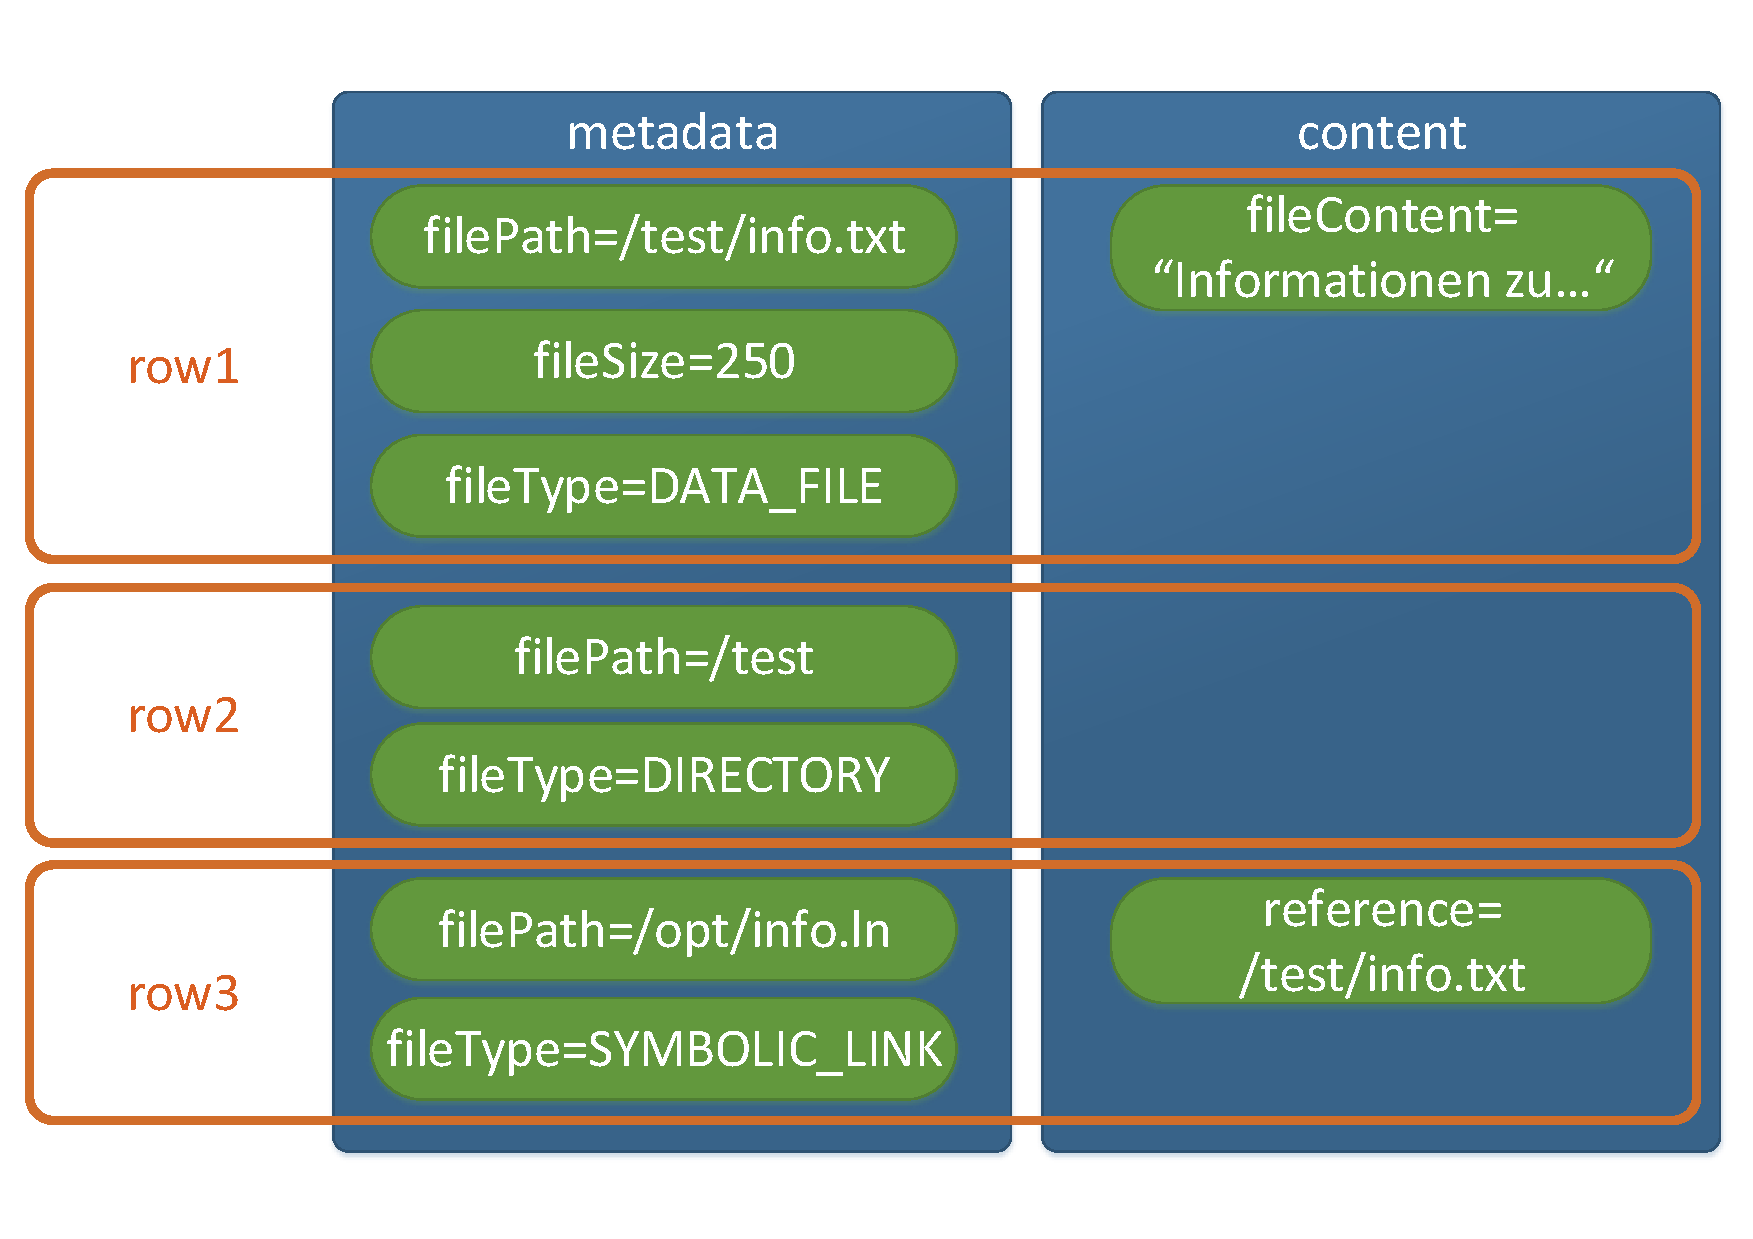
\includegraphics[width=0.8\textwidth]{./resource/hbase_data_schema_example.pdf}
  \caption{Schema-Beispiel einer HBASE Tabelle nach \cite{big_data_praxis}}
  \label{fig:hbase_schema_example}
\end{figure}

\noindent
Anhand der Abbildung werden einige Eigenschaften von HBASE sichtbar. So existieren zwei \textit{Column Families} mit den Namen \textit{metadata} und \textit{content}. Die Column Family \textit{metadata} enthält wiederum die Spalten \textit{filePath}, \textit{fileSize}und \textit{fileType}. Die Werte werden alle als Binär-Inhalt gespeichert. Eine Zeile hat dann jeweils einen eindeutigen Spaltenschlüssel, wie zum Beispiel \textit{row1}. 
Über diesen Schlüssel können die spezifischen Inhalte der einzelnen Spalten für eine bestimmte Zeile erfragt werden. Interessant hierbei ist, dass die Spaltenwerte optional sind und nicht für jede Zeile existieren müssen. So hat beispielsweise eine Datendatei, einen konkreten Inhalt, welcher in der Spalte \textit{fileContent} der Spaltenfamilie \textit{content} gespeichert werden. Ein Verzeichnis hingegen hat keinen Dateiinhalt. Daher ist in der zweiten Zeile auch kein Inhalt in der Spalte \textit{fileContent} abgelegt. In der dritten Zeile hingegen, wird ein symbolischer Link gespeichert. Dieser wiederum hat auch keinen Inhalt in der Spalte \textit{fileContent}. Dafür wird aber die Referenz auf die Originaldatei in einer weiteren Spalte gespeichert. Aufgrund der Gruppierung und Speicherung in Column Families benötigen leere Spaltenwerte auch keinen Speicherplatz. 
Ein einzelne Zelle beschreibt letztlich den Wert einer Spalte für eine konkrete Zeile. Hierbei wird zu jeder Zelle auch ein Zeitstempel gespeichert. Mithilfe diesen Zeitstempels können auch ältere Werte einer Zelle ausgelesen werden. 
So wird bei einer Modifikation einer konkreten Zelle der Wert inklusive eines neuen Zeitstempels geschrieben. Es ist jedoch immer noch möglich, ältere Zustände der Zelle zu lesen.\\
Aus Nutzersicht von Vorteil ist, dass die einzelnen konkreten Spalten innerhalb einer Spaltenfamilie nicht schon bei der Erstellung einer Tabelle angegeben werden müssen. Lediglich die Spaltenfamilien müssen initial angegeben werden und können später auch nicht mehr geändert werden. Somit kann nachträglich die Tabelle um weitere Spalten erweitert werden.\cite[S. 577]{hadoop_definitive_guide}\\

\noindent
Die Skalierbarkeit und die Partitionstoleranz wurden bei der Entwicklung von HBASE berücksichtigt. Es baut auf dem Hadoop HDFS auf und speichert darin die Daten. Analog zu HDFS, YARN oder Spark existiert auch hierbei eine Master-Slave Archtitektur über alle Knoten hinweg. Abbildung \ref{fig:hbase_cluster_architecture} zeigt die physikalische Aufteilung.\\

\begin{figure}[ht]
  \centering
  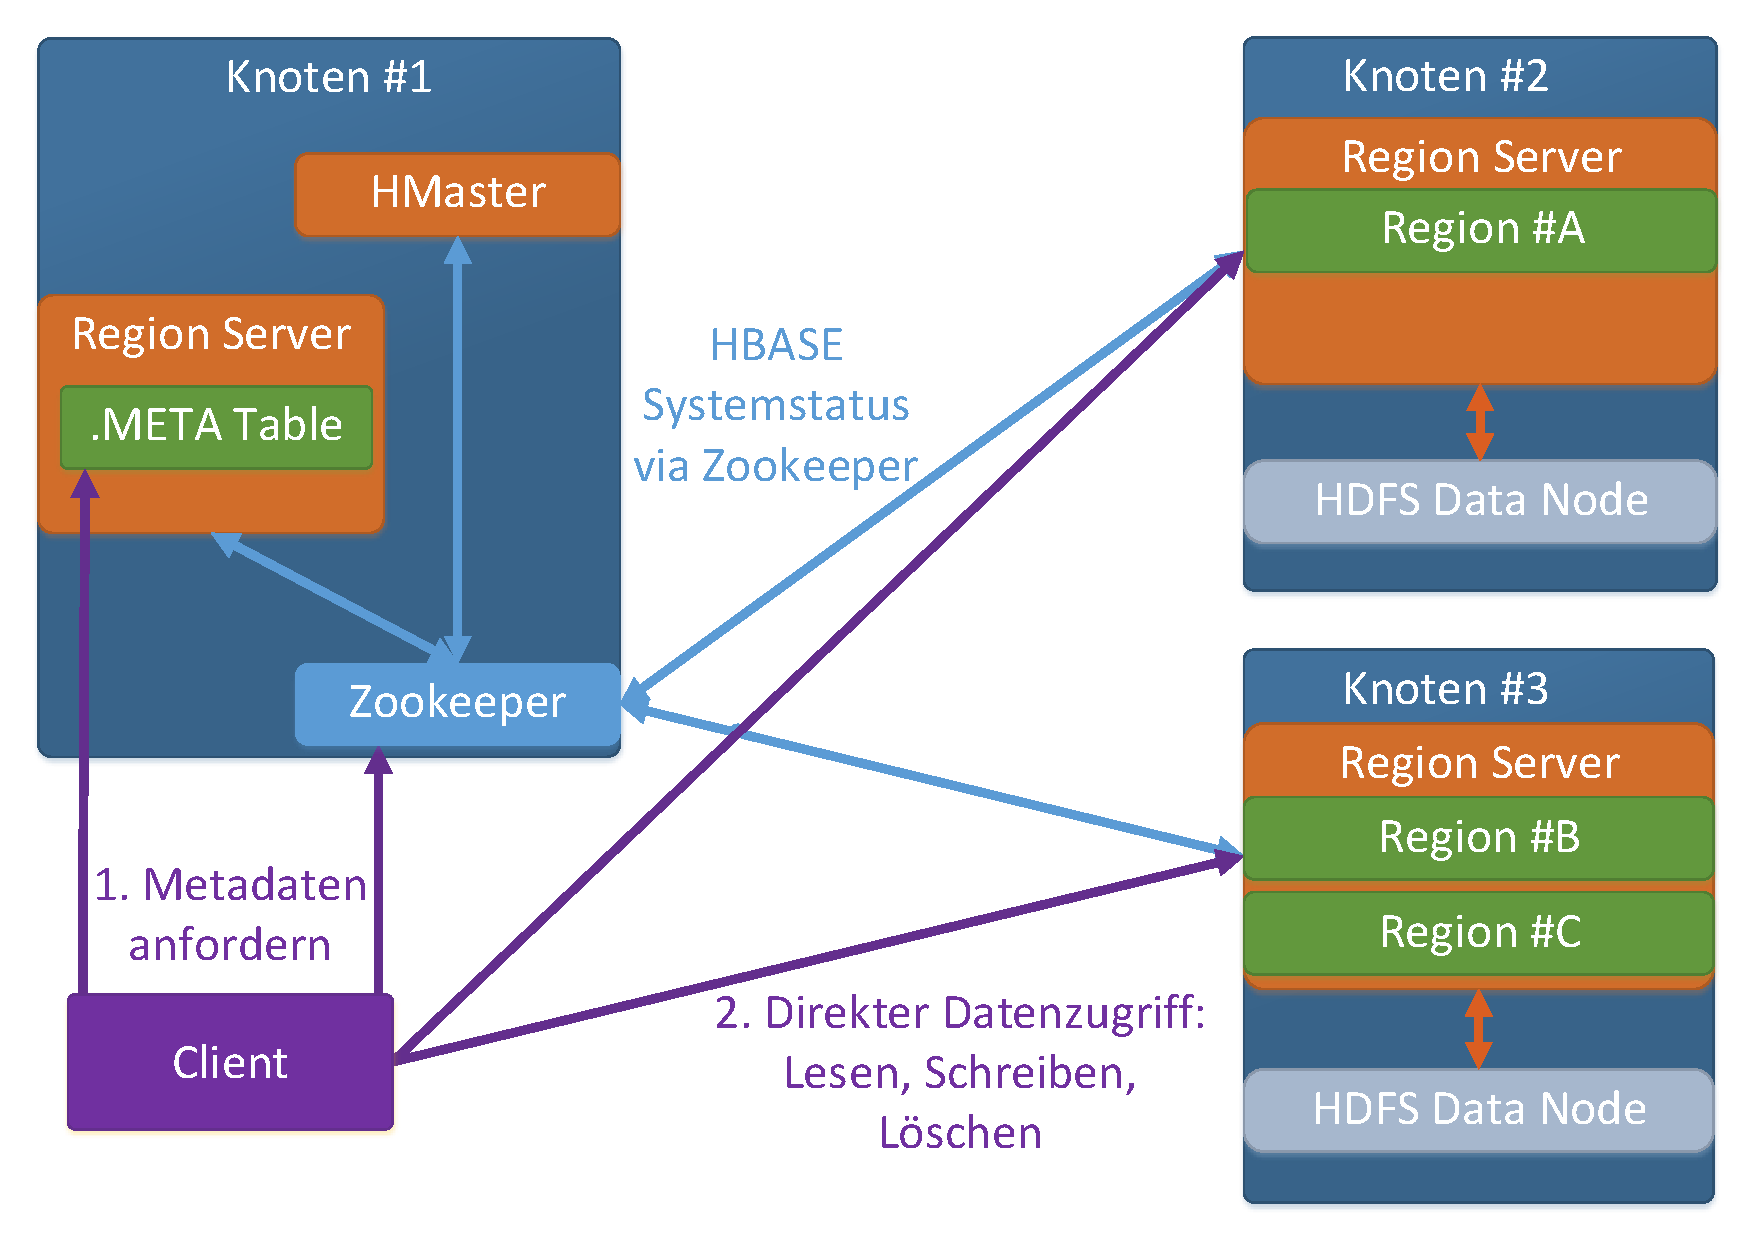
\includegraphics[width=\textwidth]{./resource/hbase_cluster_architecture.pdf}
  \caption{HBASE Datenspeicherung im Cluster}
  \label{fig:hbase_cluster_architecture}
\end{figure}

\noindent
Auf den einzelnen Knoten im Computer-Cluster laufen sogenannte \textit{Region Server}. Diese Region Server speichern jeweils unterschiedliche Teile der in HBASE angelegten Tabellen. Eine Tabelle selbst wird hierbei anhand der Zeilenschlüssel in mehrere Bereiche, den sogenannten \textit{Regions} unterteilt. Beispielsweise könnte die Region A (siehe Abbildung \ref{fig:hbase_cluster_architecture}) alle Daten einer Tabelle der Zeilen 1 bis 3000 enthalten. Die Region B wiederum enthält alle Daten der gleichen Tabelle aber von den Zeilen 3001 bis 8540. Und die Region C könnte die Daten der Zeilen 1 bis 22300 von einer anderen Tabelle enthalten. Somit kann ein Region Server mehrere Regions von gleichen oder auch unterschiedlichen Tabellen verwalten.  Das Prinzip der Datenlokalität greift auch bei HBASE. So sollte auf  jedem Knoten, auf dem ein RegionServer läuft, auch ein HDFS Data Node existieren. Dieser speichert die Daten der einzelnen Regions als Dateien im HDFS.\\

\noindent
Wenn neue Tabellen erstellt werden, oder einzelne Regions zu groß werden, dann koordiniert eine übergeordnete Instanz die Umverteilung von Daten und die Erstellung neuer Regions. Diese Instanz ist bei HBASE der sogenannte \textit{HMaster}. Es ist ein leichgewichtiger Prozess, welcher auf einem beliebigen Knoten im Cluster läuft und über Apache ZooKeeper auch den Status der einzelnen Region Server überwacht.\footnote{Die Funktionsweise von Apache ZooKeeper wird in Kapitel \ref{sec:theory_zookeeper} näher erläutert.}. Um die Ausfallsicherheit zu gewährleisten ist auch dieser Prozess redundant ausgelegt.\footnote{Über ZooKeeper kann immer der primäre HMASTER-Prozess ermittelt werden. Ist der aktive HMaster nicht mehr erreichbar, schaltet sich sich ein Backup-HMaster ein.} Darüber hinaus kümmert sich der HMaster-Prozess auch um die Restrukturierung bei Teilausfällen einzelner Region Server. 

\noindent
Wenn nun ein Client auf die Daten einer Tabelle zugreifen möchte, muss dieser wissen, auf welchem Knoten die Daten abgelegt sind. Hierfür verbindet sich der Client zuerst mit ZooKeeper und erfährt hierüber, welcher Region Server die sogenannte \textit{Meta-Tabelle} speichert.\cite[S. 579]{hadoop_definitive_guide}\\
Diese Meta-Tabelle enthält Informationen über alle Tabellen in HBASE inklusive der Region-Server und deren Regions die sie bereitstellen. Anhand dieser Metadaten kann der Client dann direkt die benötigten Daten an den entsprechenden Region Servern anfordern.\\
Dieses Vorgehen scheint für den Zugriff auf wenige Daten etwas aufwendig. Es skaliert aber sehr gut bei großen Datenmengen, da kein Flaschenhals vorhanden ist. Normalerweise speichert der Client die angeforderte Meta-Tabelle temporär, so dass er bei nachfolgenden Anfragen direkt au die entsprechenden Region Server zugreifen kann.\\ 

\noindent
Im Rahmen dieser Thesis wird HBASE beispielsweise verwendet um Metadaten zu speichern. Diese werden wiederum mit Apache Spark ausgelesen und verarbeitet. Hierbei kann das Prinzip der Datenlokalität sehr gut genutzt werden. Denn in der Theorie ist es durchaus möglich die HDFS Data Nodes, die Spark Worker und die HBASE Region Server getrennt auf unterschiedlichen Knoten auszuführen. Aber gerade dies macht keinen Sinn, da sonst immer wieder Daten über das Netzwerk transportiert werden müssen und dieses dann zum Flaschenhals der Verarbeitung wird.\\
Sinnvoll ist es nämlich HDFS Data Nodes auf den Knoten auszuführen, wo auch die Region Server ausgeführt. Darauf aufbauend sollten dann gerade auch die Spark Worker auf den Knoten die Datenverarbeitung ausführen, auf welchen die Region Server laufen. Dadurch können im besten Fall die Daten, welche durch Apache Spark benötigt werden, direkt von dem lokalen HBASE Region Server bereitgestellt werden. Dieser erhält die Daten wiederum von dem lokal laufendem Data Node. Somit können die Daten direkt auf dem Knoten verarbeitet werden, wo sie auch gespeichert sind und müssen nicht über das Netzwerk an andere Knoten gesendet werden.\footnote{Sie auch Kapitel \ref{sec:theory_yarn} und Kapitel \ref{sec:theory_spark}.} Die Koordinierung ist aber entsprechend komplex und viel wichtiger ist noch, dass jede einzelne Implementierung zur Prozessierung der Daten auch das Prinzip der Datenlokalität unterstützt.\\

\noindent
TODO: Erstellung eines adäquaten Zeilenschlüssels und dessen Auswirkungen (numerische Sortiertung, Hot Spot, ...) -> Dies könnte aber dann in Kapitel 4 oder 5 beschrieben werden!


\section{Apache ZooKeeper}
\label{sec:theory_zookeeper}

Innerhalb eines Computer-Clusters zur verteilten Datenverarbeitung existiert oftmals das Problem, dass sich die einzelnen Komponenten koordinieren müssen. Beispielsweise teilt HBASE die Daten auf mehrere RegionServer auf, welche wiederum auf den einzelnen Knoten laufen. Doch welche Instanz koordiniert diese Aufteilung? Ein anderes Problem ist der Datenzugriff. Ein Client möchte eine Zeile einer bestimmten Tabelle auslesen. Woher weiß der Client, welchen konkreten Knoten er anfragen muss, um genau diese Zeile zu erhalten? In den meisten Fällen existiert hierzu eine bestimmte Instanz, welche die Koordinierung der Knoten übernimmt. Beispielsweise gibt es bei HBASE den HMaster, welcher die Koordinierung übernimmt. Das Problem ist hierbei, dass auch der Knoten auf dem diese Master-Instanz läuft ausfallen kann und das komplette System zum erliegen bringt. Diese Master-Instanzen im allgemeinen sind kritische Komponenten und können als Single-Point-of-Failure zu einem Stillstand des kompletten Systems führen. Um solche Totalausfälle zur vermeiden, müssen bestimmte Automatismen definiert werden, wie sich die Knoten selbst organisieren können, um einen Ausfall beliebiger Knoten zu überstehen.\\

\noindent
An dieser Stelle bietet \textit{Apache ZooKeeper\texttrademark\thinspace} Mechanismen an, wie sich die einzelnen Knoten in einem verteilten System organisieren und Informationen verteilt synchronisieren können. Aus logischer Sicht stellt ZooKeeper einen Service zu Verfügung. Dieser Service ermöglicht das Speichern von Informationen strukturiert als Verzeichnis mit einzelnen Dateien. Bei den Informationen handelt sich normalerweise um wichtige Konfigurationen, welche im Cluster verteilt werden müssen und zentral über ZooKeeper aktualisiert werden können. Jeder Client, der sich mit ZooKeeper innerhalb des Computer-Clusters verbindet, sieht die gleiche Konfiguration und kann bei Bedarf auch bestimmte Konfigurationen ändern.\cite[S. 4 ff]{professional_hadoop} \\
Aus Sicht des Entwicklers, stellt dieser Service immer die aktuellen Informationen im Cluster zu Verfügung. Wie der Service dies bewerkstelligt ist ein Implementierungs-Detail. Neben dem bereits erwähnten Konfigurationsmanagement bietet ZooKeeper auch einen Naming-Service oder auch die Möglichkeit den Live-Status einzelner Knoten zu überwachen.\cite{zookeeper_essentials}\\
Wie bei HBASE in Kapitel \ref{sec:theory_hbase} bereits erwähnt, kann ein Client sich mit ZooKeeper verbinden und erhält über ZooKeeper den aktuellen Knoten, welcher die Metadaten zu allen Tabellen in HBASE Speichert. Ein anderes Beispiel zeigt die Backup-Instanz des HMaster-Prozesses. Dieser prüft über ZooKeeper den Status des primären HMaster-Prozesses und wird informiert, wenn letzterer nicht mehr verfügbar ist. Daraufhin propagiert sich die Backup-Instanz als neuen HMaster-Prozess im Cluster, um so die Funktionsfähigkeit von HBASE aufrecht zu erhalten. Abbildung \ref{fig:zookeeper_dir} zeigt die Verzeichnisstruktur, welche stark an ein Unix-Verzeichnis erinnert. Wobei die einzelnen Einträge sogenannten \textit{ZNodes} entsprechen.\footnote{Siehe auch \url{http://zookeeper.apache.org/doc/r3.5.4-beta/zookeeperOver.html}, Stand: 26.7.2018} \\

\begin{figure}[ht]
  \centering
  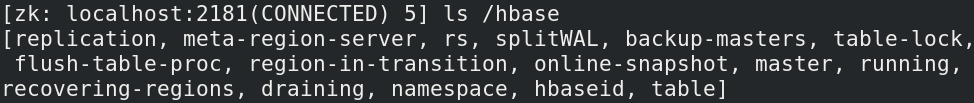
\includegraphics[width=\textwidth]{./resource/zookeeper_dir.png}
  \caption{Gespeicherte Informationen von HBASE in ZooKeeper}
  \label{fig:zookeeper_dir}
\end{figure}


\noindent
Normalerweise ist Zookeeper auf mehreren Knoten im Cluster installiert. Sie bilden ein sogenanntes \textit{ZooKeeper Ensemble} und bestehen zumeist aus 3 oder 5 Einzelinstallationen auf beliebigen Knoten. Ein ZooKeeper Ensemble, welches für die gleiche Anwendungsdomäne zuständig ist, wird auch \textit{Quorum} genannt. Innerhalb eines Quorums gibt es einen Leader und mehrere Follower, die sich die gleichen Konfigurationsinformation teilen. Fällt der Leader aus, können die Follower einen neuen Leader bestimmen.\cite{zookeeper_essentials}\\

\section{Apache Solr und Lucene}
\label{sec:theory_solr}
\textit{Apache Solr\texttrademark\thinspace} ist eine skalierbare und performante Plattform zur Datensuche. Die Daten werden vorher indexiert und könne extrem schnell durchsucht werden.\cite{solr_search}\\
Dadurch kann der forensische Analyse im Rahmen der Thesis schnell und einfach Millionen von Datensätzen nach bestimmten Stichwörtern durchsuchen.\\

\noindent
Solr besitzt einen \textit{Cloud-Mode}, welcher es ermöglicht die indexierten Daten verteilt auf mehreren Rechnern zu speichern. Dieser Cloud-Mode wird auch bei der Integration in die Analyseplattform genutzt. Die Hortonworks Dataplatform, welche auf dem Computer-Cluster, installiert ist liefert ein optionales Solr-Paket mit. Primär wird dieses Paket genutzt, um eine performante Suche im HDFS-Dateisystem zu ermöglichen. Jedoch können beliebige Daten in der Solr-Cloud indexiert werden, sobald diese einmal im Computer-Cluster installiert wurde. Darüber hinaus nutzt Solr im Cloud-Mode das bereits beschriebene Zookeeper-Projekt\footnote{Siehe Kapitel \ref{sec:theory_zookeeper}.} zur Koordinierung und Überwachung der einzelnen Knoten.\\
Innerhalb des Cloud-Modes werden die oben beschriebenen Indizes in mehrere sogenannte \textit{Shards} aufgeteilt. Ein einzelner Shard ist hierbei ein Teil des Indexes, welcher unabhängig von den anderen Shards durchsucht werden kann. So kann bei einer Suchanfrage die Suche parallel auf alle Shards verteilt werden. Einzelne Shards können wiederum auf anderen Knoten repliziert werden, um die Ausfallsicherheit zu gewährleisten. Solr spricht hierbei von Cores. Ein Core ist die physikalische Representation eines logischen Shards auf einem konkreten Knoten. Alle logischen Shards bilden zusammen den Index, welcher bei Solr als sogenannte \textit{Collection} dargestellt wird.\cite{solr_cloud_scaling}\\

\noindent
Jedes Dokument, welches in einer Collection indexiert werden soll, wird genau einmal ein eines der logischen Shards aufgeteilt. Hierbei wird zuerst anhand einer Strategie, wie beispielsweise mittels Hashwertermittlung eines eindeutigen Dokument-Keys, entschieden in welchen Shard das Dokument aufgenommen werden sollen. Ein logischer Shard wird abermals aufgeteilt in mehrere Replicas, den bereits erwähnten Cores auf den einzeln Knoten. Für jeden logischen Shard wird ein \textit{Leader}-Knoten bestimmt.\footnote{Diese Leader werden mittels Zookeeper im Cluster propagiert.}. Dieser Leader-Knoten speichert einen physikalischen Core des logischen Shards und indexiert im nächsten Schritt das Dokument. Sobald der Index neu aufgebaut wurde, wird die Aktualisierung an die anderen Knoten weitergesendet, welche wiederum eine Replica (Core) des logischen Shards speichern.\cite[S. 867 ff]{solr_ref_guide}\\ 
Abbildung \ref{fig:solr_cluster_architecture} skizziert die Skalierung im Computer-Cluster.\\

\begin{figure}[ht]
  \centering
  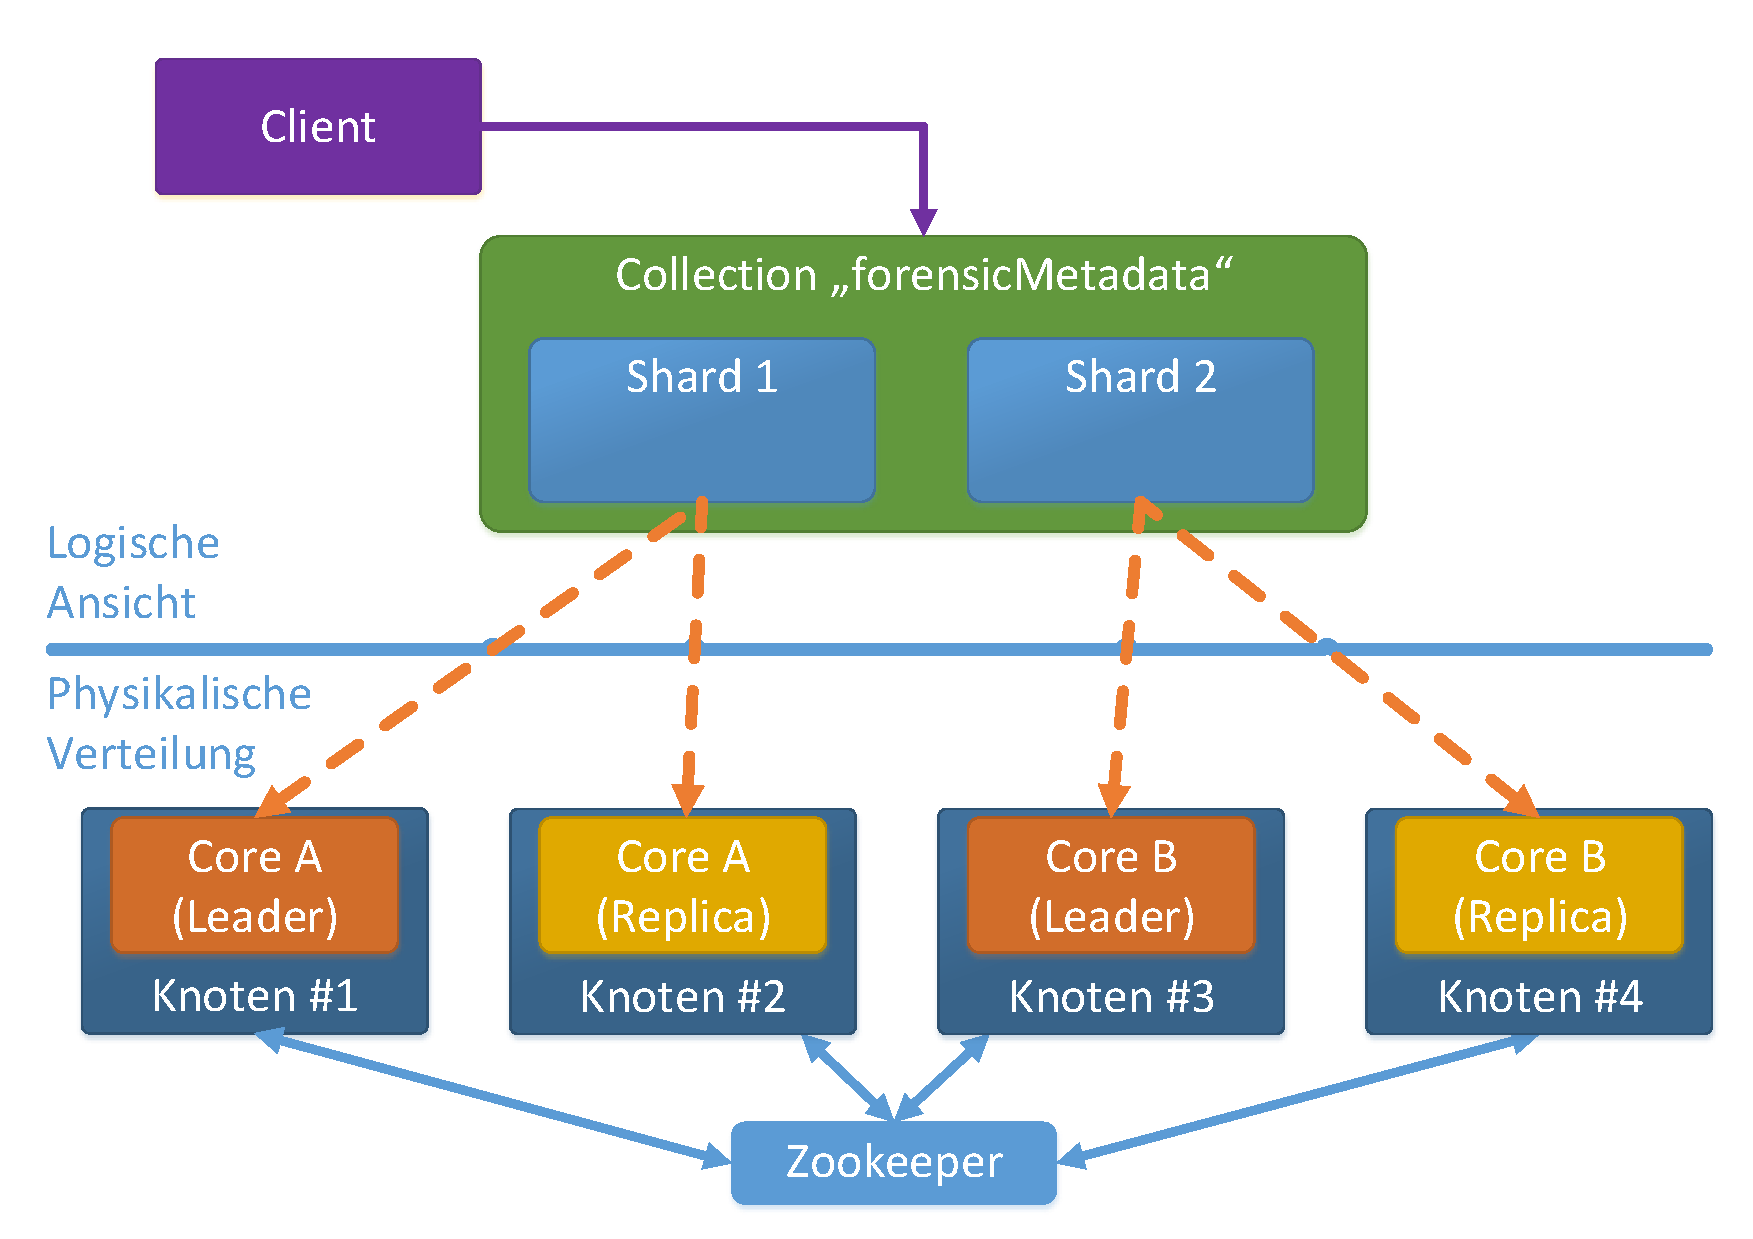
\includegraphics[width=\textwidth]{./resource/solr_cluster_architecture.pdf}
  \caption{Solr Cloud-Mode im Cluster}
  \label{fig:solr_cluster_architecture}
\end{figure}


\noindent
Im Allgemeinen ist ein Suchsystem in mehrere Analyseschritte aufgeteilt. Ein Großteil dieser Verarbeitungsschritte wird nicht von Solr selbst übernommen. Vielmehr baut Solr auf dem Open-Source Projekt \textit{Apache Lucene\texttrademark\thinspace} auf und erweitert Lucene letztlich um eine skalierbare Infrastruktur und diverse Schnittstellen zur Verarbeitung der Daten.\\
Zu Beginn liegen beliebige Daten in Form von Dateien oder Dokumente vor. Diese Daten durchlaufen eine textuelle Aufbereitung bevor sie indexiert werden können.\\ 
Bei der Textanalyse wird der relevante Text aus den Daten extrahiert. Hierbei hängt die Extraktion der Daten auch davon ab, ob die Daten strukturiert, semistrukturiert oder unstrukturiert sind. Anhand der Dateiformate können dann diverse Bibliotheken genutzt werden, um Daten zu extrahieren. Beispielsweise kann mithilfe von \textit{Apache PDFBox\textsuperscript{\textregistered}}\footnote{Siehe \url{https://pdfbox.apache.org/}, letzter Zugriff: 01.08.2018} Text aus PDF-Dokumenten extrahiert werden. Mithilfe der \textit{Geospatial Data Abstraction Library (GDAL)}\footnote{Siehe \url{https://pdfbox.apache.org/}, letzter Zugriff: 01.08.2018} können Geo-Positionen aus den EXIF-Metadaten von JPEG-Bildern extrahiert werden. Oder mithilfe \textit{Tesseract OCR}\footnote{Siehe \url{https://github.com/tesseract-ocr/tesseract}, letzter Zugriff: 01.08.2018} könnte auch lesbarer Text direkt aus Bildern extrahiert werden.\cite[S. 39]{solr_search}\\

\noindent
Im nächsten Schritt wird dieser extrahierte Text aufbereitet. Diese Aufbereitung hängt auch stark von dem spezifischen Anwendungsfall und den Daten selbst ab. Im Allgemeinen werden Satzzeichen und überflüssige Füllwörter entfernt und Großbuchstaben werden in Kleinbuchstaben umgewandelt. Darüber hinaus kann auch eine Stammformreduktion durchgeführt werden. Darauf aufbauend kann der Text weitergehend analysiert werden. Beispielsweise könnten Redewendungen erkannt oder Synonyme einzelner Wörter identifiziert werden.\cite[S.44]{solr_search}\\

\noindent
Nach der Aufbereitung des Textes erfolgt die Erstellung eines sogenannten \textit{Inverted Indexes}. Ein \textit{Inverted Index} ist ähnlich aufgebaut, wie ein Stichwortverzeichnis. Jedes Wort wird darin mit den Verweisen zu den Vorkommen in den einzelnen Dokumenten versehen. Auf Basis dieses Indexes können sehr schnell alle Dokumente gefunden werden, welche das gesuchte Wort enthalten.\cite[S. 47]{solr_search}

\noindent
Im nächsten Schritt können nun Suchanfragen auf die erstellen Indizes durchgeführt werden. Aber auch hier gibt es unterschiedliche Modelle, wie die relevanten Dokumente ermittelt werden und vor allem auch in welcher Reihenfolge die Ergebnismenge zurückgeliefert wird.\\
Hier existiert das sogenannte \textit{Boolean Model} auf Basis der booleschen Algebra. Beispielsweise könnte eine forensische Suchanfrage lauten: Suche alle Bilder oder Videos, welche das Wort \textit{Unfall} im Dateinamen haben aber nicht kleiner sind als 1 MB. Diese Suchanfrage wird in einen booleschen Ausdruck überführt und die Dateien werden zurückgeliefert. Allerdings liefert dieses Modell keine Aussage über die Reihenfolge der Ergebnismengen. Hierzu gibt es komplexere Suchmodelle, wie das sogenannte \textit{Vector Space Model}. Es basiert auf gewichtete Faktoren und ermöglicht es für jedes Dokument der Ergebnismenge die Trefferwahrscheinlichkeit zu ermitteln. Nach dieser Bewertung wird die Reihenfolge der Ergebnisse ermittelt. Beispielsweise sollte ein Dokument eine höhere Bewertung erhalten, wenn das gesuchte Wort mehrfach im Dokument vorhanden ist.\cite[S. 47 ff]{solr_search}\\

\noindent
Apache Solr und Lucene sind beide in Java implementiert. Daher gibt es auch einen Java Client, zur Durchführung von Suchanfragen. Andererseits existiert auch eine REST-Schnittstelle. Damit können Anfragen simpel und schnell in beliebige Websites integriert werden, oder direkt mit dem Kommandozeilentool \textit{curl} durchgeführt werden. Hierbei können die Anfragen in XML oder JSON formatiert sein. Ein simples Beispiel zeigt nachfolgende Anfrage (siehe Abbildung \ref{fig:solr_request}).\\

\begin{figure}[ht]
  \centering
  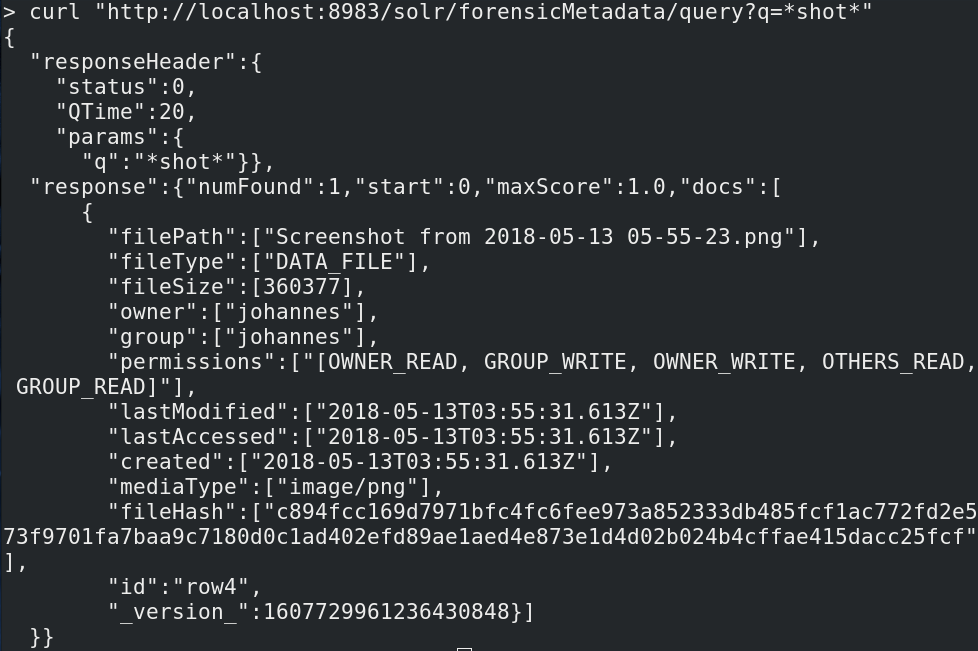
\includegraphics[width=\textwidth]{./resource/solr_request.png}
  \caption{Solr-Suchanfrage via \textit{curl}}
  \label{fig:solr_request}
\end{figure}

\noindent
Die Solr-Instanz ist unter \url{localhost:8983} erreichbar ist. Die Suchanfrage selbst wird auf der Collection \textit{forensicMetadata} ausgeführt. Es soll in allen Feldern nach einem Vorkommen von dem Wort \textit{shot} (\textit{q=*shot*}) gesucht werden. Die Antwort ist im JSON-Format definiert. Unter anderem wird die Anzahl der Treffer (\textit{numFound:1}) mitgeliefert. Bei dieser konkreten Anfrage, wurde ein Bild mit dem Dateinamen \textit{Screenshot...} gefunden. 
\chapter{Datenspeicherung}
\label{ch:data_persistence}

\section{Allgemeiner forensischer Analyseprozess}
\label{sec:common_analysis_process}
Im Praxisteil dieser Arbeit soll eine Analyseplattform auf Basis von Apache Hadoop aufgebaut werden. Diese Analyseplattform dient zur Auswertung sichergestellter Asservate und dem Auffinden von Beweisen in großen Datenmengen. Hierbei behandelt die Analyseplattform aber nur einen Teil der Arbeitsvorgänge während einem forensischen Analyseprozess.\\

\noindent
Abbildung \ref{fig:digital_forensics_process} skizziert einen allgemeinen forensischen Analyseprozess für digitale Beweismittel.\cite[S.16]{digital_forensics} Die grün hinterlegten Schritte definieren den Arbeitsbereich, bei welchen die hier entwickelte forensische Analyseplattform den Forensiker unterstützen kann.\\ 
\begin{figure}[ht]
  \centering
  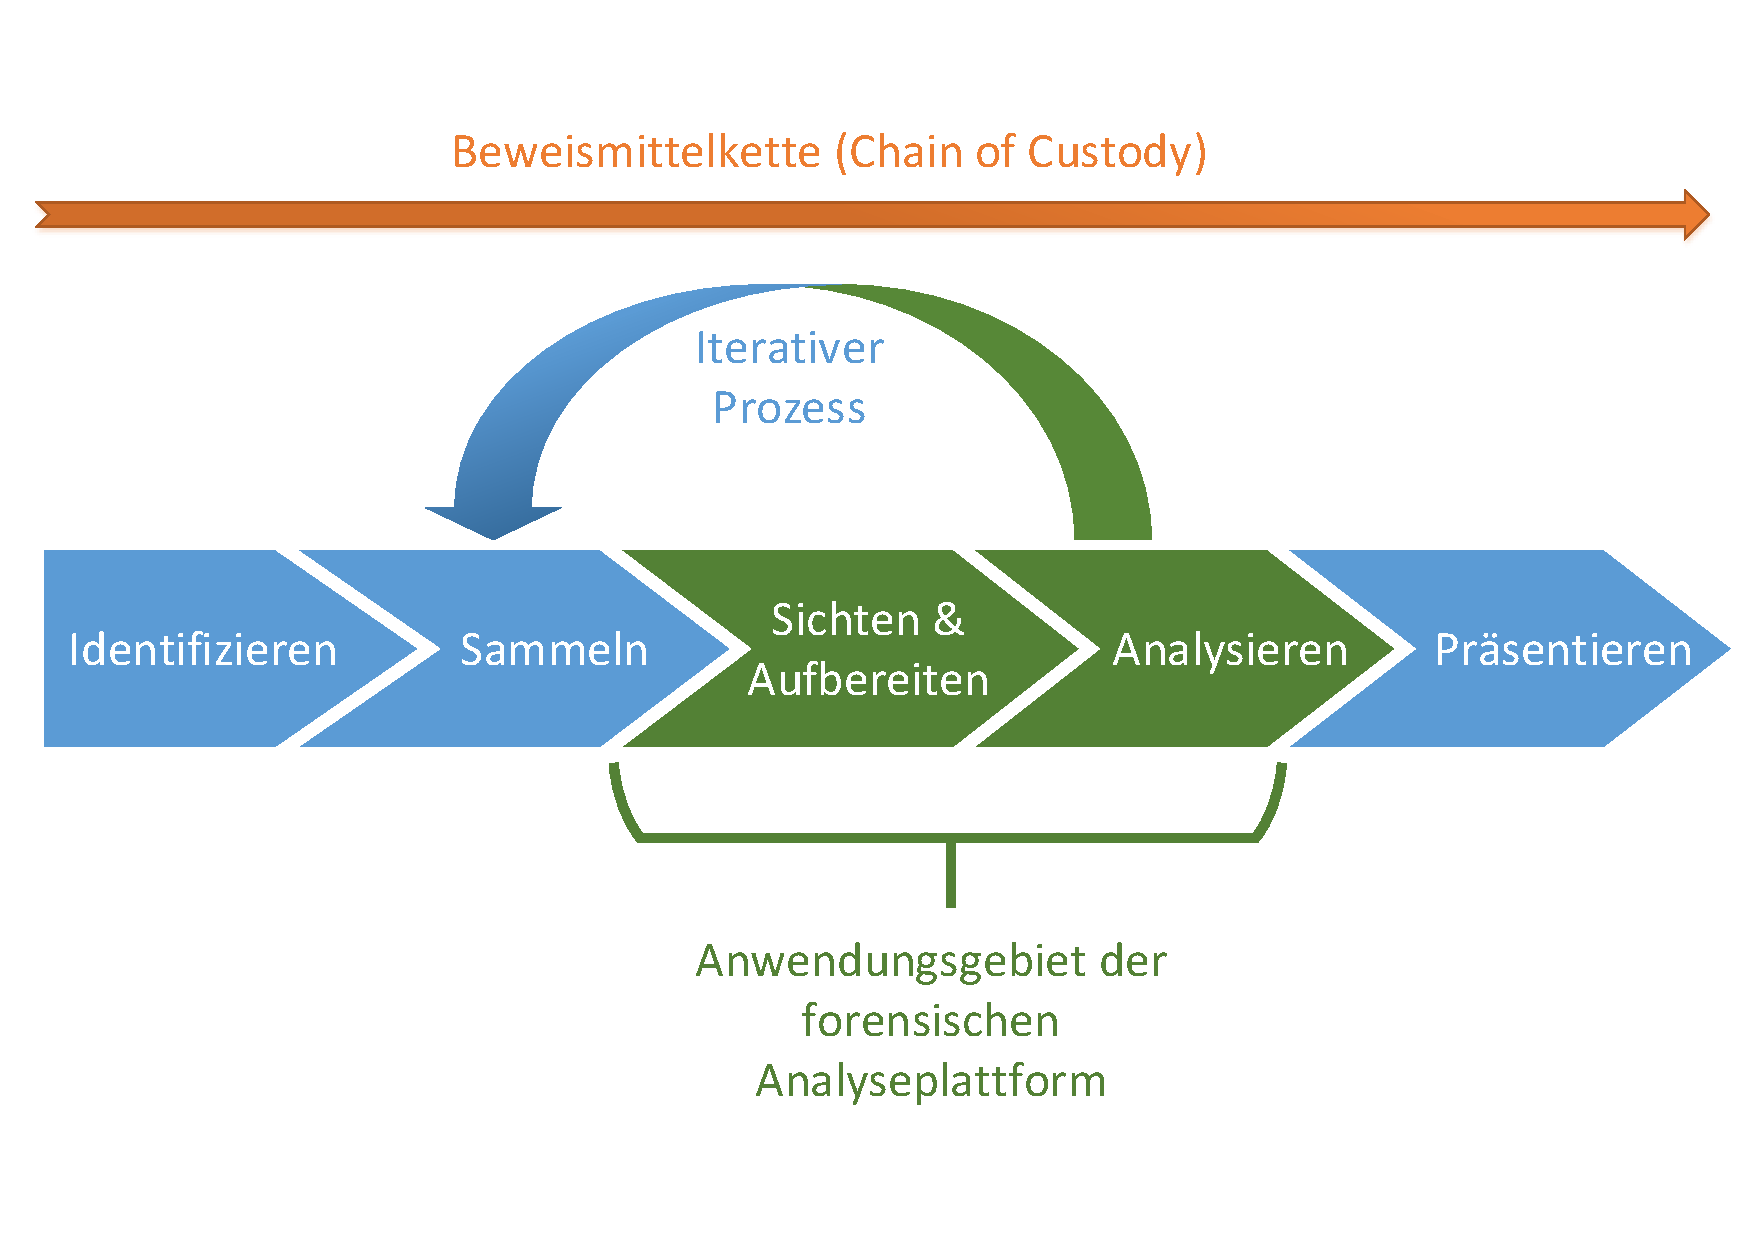
\includegraphics[width=\textwidth]{./resource/digital_forensics_process.pdf}
  \caption{Forensischer Analyseprozess für digitale Beweismittel (Vgl. \cite[S.16]{digital_forensics})}
  \label{fig:digital_forensics_process}
\end{figure}


\noindent
Zu Beginn existiert ein Vorfall oder ein Tatverdacht für eine Straftat. In einem nachfolgenden Schritt ermittelt beispielsweise die Staatsanwaltschaft. Im Ermittlungsverlauf wird darauf der Tatort untersucht oder auch bei Tatverdächtigen nach Hinweisen für die Tat und gegebenenfalls deren Tathergang gesucht. Dieser Schritt beschreibt die Identifikationsphase aus Abbildung \ref{fig:digital_forensics_process}. Hierbei geht es um die Identifikation von potentiellen Beweismitteln, welche sichergestellt oder beschlagnahmt werden sollen.\cite[S. 17-24]{digital_forensics}.\\ In der Forensik wird häufig hypothesenbasiert vorgegangen. So entwickelt der Ermittler eine Hypothese, wie eine möglich Straftat begangen wurde und wer diese begangen haben könnte. Darauf aufbauend überlegt er sich, welche Spuren für oder gegen diese Hypthese sprechen und welche möglichen Beweismittel eben diese Spuren enthalten könnten (z.B. Kommunikationsdaten auf dem PC oder Bildmaterial auf einem Mobiltelefon).\\

\noindent
Im zweiten Schritt aus Abbildung \ref{fig:digital_forensics_process} geht es um das Vereinnahmen von potentiellen Beweismitteln. Hierbei werden identifizierte Datenträger und Geräte sichergestellt oder beschlagnahmt. In dieser Phase werden beispielsweise auch schon forensisch korrekte Datenträgerabbilder erstellt, auf welchen dann später eine Datenanalyse ausgeführt werden kann.\cite[S. 24-33]{digital_forensics} In vielen Fällen, beispielsweise bei Unternehmensservern, werden nicht die Geräte selbst sichergestellt, sondern nur wichtige Teile der Daten forensisch korrekt kopiert. Auch hier findet teilweise schon eine Vorselektion statt, welche Daten benötigt werden und welche Daten für den konkreten Fall irrelevant sind.\\

\noindent
Die dritte Phase aus Abbildung \ref{fig:digital_forensics_process} behandelt das Sichten und Aufbereiten der sichergestellten Daten. Gerade bei großen unstrukturierten Datenmengen erfolgt in dieser Phase auch eine Vorselektion, um die Datenmenge nochmals einzugrenzen. Dies kann automatisiert oder auch manuell erfolgen.\cite[S. 33-39]{digital_forensics}\\
An dieser Stelle beginnt das Anwendungsgebiet der hier entwickelten forensische Analyseplattform. So können alle gesammelten Daten in die forensische Analyseplattform importiert und prozessiert werden. Darauf kann über eine allgemeine Suche nach spezifischen Stichworten, Hashsummen oder Zeitpunkten gesucht werden. 
Dies soll dem Ermittler das Auffinden von fallreleventen Daten erleichtern. Die meisten bekannten forensischen Analysetools bieten ebenfalls eine Stichwortsuche an, weil damit große Datenmengen schnell nach bestimmten Kriterien gefiltert werden können.\cite[S. 116-123]{handbook_digital_forensics}\\
In dieser Phase werden aber auch gelöschte, verschlüsselte oder verschleierte Daten wiederhergestellt oder entschlüsselt, sofern dies möglich ist. Eine klassische Methode ist beispielsweise auch das sogenannte \textit{File Carving} auf Datenträgern.\cite[S. 38-39]{digital_forensics}\footnote{Beim File Carving wird versucht logisch zusammenhängende Daten allein anhand des Dateiinhalts zu rekonstruieren, ohne die Dateisystemmetadaten zu nutzen. 
Die Methode wird gerne angewendet, wenn das Dateisystem nicht wiederherstellbar ist oder wenn gelöschte Dateien auf bereits freigegebenen Speicherbereichen gesucht werden.} Diese Art von Datenaufbereitung beherrscht die hier entwickelte forensische Analyseplattform derzeit noch nicht.\footnote{Es wäre aber durchaus möglich diverse Methoden der Datenaufbereitung zu implementierten. Siehe auch Kapitel \ref{ch:ausblick}.}\\

\noindent
Auch in der anschließenden Analysephase kann die hier entwickelte forensische Analyseplattform genutzt werden (siehe Abbildung \ref{fig:digital_forensics_process}). In dieser Phase werden die aufbereiteten Daten detailliert analysiert, um Informationen zu erhalten die für oder gegen einen bestimmten Tathergang sprechen.\cite[S. 39-45]{digital_forensics} Anhand dieser Informationen werden die eingangs beschriebenen Hypothesen zu möglichen Tathergängen verifiziert. Bei einer Analyse werden aus den Daten komplexe Zusammenhänge und Beziehungen erarbeitet. Beispielsweise werden aus den Rohdaten Kommunikationsverläufe auf Basis von E-Mails oder zeitliche Abläufe basierend auf Zeitstempelanalysen erstellt.\cite[S. 33-39]{digital_forensics}\\
Hierbei geht es auch darum die Aussagekraft eines potentiellen Beweismittels zu ermitteln. So könnte beispielsweise urheberrechtsverletzendes Material auf einem Datenträger eines PCs gefunden werden. Allerdings kann die Aussagekraft dieses potentiellen Beweismittels sehr gering sein, wenn das System bereits durch Schadsoftware kompromittiert wurde.\\
Einige Analyseschritte können automatisiert werden und sind daher prädestiniert für die hier entwickelt Analyseplattform (siehe auch Kapitel \ref{ch:data_processing}).\\

\noindent
Bei der Analyse können wieder Verbindungen zu neuen potentiellen Beweismitteln gefunden werden, welchen dann wieder über den forensischen Analyseprozess vereinnahmt und aufbereitet werden. Daher ist der Prozess auch iterativ anzusehen. Gerade durch die Nutzung der forensischen Analyseplattform sollen diese Iterationen verkürzt werden, indem durch die parallelisierte Prozessierung Zeit eingespart werden soll.\\

\noindent
In der letzten Phase des Analyseprozesses müssen die Ermittlungsergebnisse visuell aufbereitet werden, um sie auch vor Gericht präsentieren zu können. Letztlich muss ein Analysebericht erstellt werden, welcher einerseits die Ergebnisse enthält und andererseits nachvollziehbar beschreibt, wie diese Analyseergebnisse zustande gekommen sind.\footnote{Der Bericht sollte so geschrieben sein, dass andere Parteien oder Ermittler die gleichen Ergebnisse reproduzieren können.}\cite[S. 45-47]{digital_forensics} Viele Analysetools, unter anderem auch das hier genutzte Referenztool \textit{Autopsy}, ermöglichen die halbautomatische Erstellung von Analyseberichten. Die hier entwickelte Analyseplattform kann dies derzeit noch nicht. Bei einer Weiterentwicklung der Analyseplattform wäre diese Funktionalität aber durchaus brauchbar.\\

\noindent
Ein primärer Aspekt bei dem allgemeinen forensischen Analyseprozess aus Abbildung \ref{fig:digital_forensics_process} ist letztlich die Dokumentation der Beweismittelkette. Mit ihr steht und fällt die Aussagekraft der Ergebnisse aus einer forensischen Analyse. Daher muss bei der Dokumentation der Asservate lückenlos festgehalten werden, wie diese aufbereitet wurden und gegen unberechtigten Zugriff oder ungewollte Modifikationen gesichert wurden. Nachfolgende Liste liefert wichtige Kriterien, die im Protokoll zur Beweismittelkette festgehalten werden sollten:
\begin{itemize}
\item Die Ermittler, welche das Beweismittel sichergestellt und später analysiert haben.
\item Die Prozesse, Datenaufbereitungen und Analysen, welche durchgeführt wurden.
\item Die Zeitpunkte der Sicherstellung, Aufbereitung und der Analyse.
\item Die Umstände, wie das Beweismittel sichergestellt wurde.
\item Gründe, wieso das Beweismittel sichergestellt wurde.
\item Transportwege und Lagerstätten der Beweismittel.
\item Personen die Zugang zu den Beweismittel hatten und allgemeine Informationen, wie die Beweismittel vor unbefugtem Zugriff geschützt wurden.
\end{itemize}

\noindent
Ein sehr wichtiger Punkt bei der Dokumentation der Beweismittelkette ist die Verifikation der Datenintegrität der Asservate während des gesamten Analyseprozesses. Dies wird primär durch die Prüfung mittels kryptografischer Hashes erreicht. Letztlich dienen diese zum Schutz vor einer Modifikation des Beweismittels. Das Ändern von Asservaten oder deren Kopien sollte eigentlich immer vermieden werden. In vielen Fällen ist dies jedoch notwendig, um beispielsweise defekte Datenstrukturen wiederherstellen zu können. Bei solchen bewussten Datenänderungen ist eine entsprechende Dokumentation erforderlich.\\ 

\noindent
Bei der Analyse mit der hier entwickelten Analyseplattform muss auch die Beweismittelkette entsprechend dokumentiert werden. Die derzeitige Implementierung der forensischen Analyseplattform behandelt diesen Aspekt noch nicht. Aber auch hier könnte in einer Weiterentwicklung eine Beweismittelkette erstellt werden, welche die einzelnen Verarbeitungsprozesse, Zeitpunkte und Nutzerzugriffe dokumentiert. Da das System gegen unbefugten Zugriff gesichert werden muss, könnten in einer zukünftigen Weiterentwicklung Maßnahmen zur Nutzeridentifikation und Authentifizierung implementiert werden (siehe Kapitel \ref{sec:secure_platform}). Diese Mechanismen protokollierten einzelne Nutzeranmeldungen und Datenzugriffe, welche dann wiederum als Grundlage zur automatischen Erstellung eines Protokolls zur Beweismittelkette dienen könnten.\\

\section{Klassisches Analysevorgehen}
\label{sec:common_analysis_approach_part1}
Um die fachlichen Anforderungen an das Analyse-System herauszuarbeiten, soll das herkömmliche Analysevorgehen mit einem vergleichbaren Open-Source Analysewerkzeug betrachtet werden.\\
Die Ausgangslage liefern einige Datenträgerabbilder aus diversen Testszenarien. Diese Datenträgerabbilder sind bezogen auf den forensischen Analyseprozess aus Abbildung \ref{fig:digital_forensics_process} die Grundlage für dir dritte Phase - dem Sichten und Aufbereiten der Daten.

\noindent
Bei gängigen Analysevorgehen werden beispielsweise die Datenträgerkopien mit Betriebssystemprogrammen unter Linux oder mithilfe des Open-Source Analysetools \textit{Autopsy}\footnote{Siehe Link: \url{https://www.sleuthkit.org/autopsy/}. Letzter Zugriff: 10.8.2018. Es wird die Version 4.7.0 in der 64-bit Variante unter Windows 10 Pro genutzt.} unter Windows analysiert. Im kommerziellen Bereich existieren etliche weitere Analyse-Tools mit größerem Funktionsumfang. Nachfolgend wird Autopsy als Referenzsystem unter Windows betrachtet, da es eines der bekanntesten Analysewerkzeuge unter den kostenfreien Open-Source Programmen ist. \\ 

\noindent
Die Datenträgerabbilder können in unterschiedlichen Dateiformaten vorliegen. Mithilfe klassischer Open-Source Anwendungen, wie beispielsweise \textit{dd}\footnote{dd ist ein bekanntes Werkzeug zum Kopieren von Daten, welches unter den meisten Unix-basierten Betriebssystemen läuft. Damit können auch ganze Partitionen in einzelne logische Dateien kopiert werden.} können Abbilder im sogenannten \textit{RAW}-Format erstellt werden. Von \textit{dd} existiert auch eine forensische Variante \textit{dcfldd}, welche beim Kopieren auch noch Hashsummen zur Verifikation berechnet.\cite{linux_forensics}  Andere Tools, wie der \textit{FTK-Imager} können auch Datenträgerabbilder in speziellen Container-Formaten erstellen und lesen. Zum Beispiel gibt es das \textit{EnCase Physical}-Format mit der Dateiendung \textit{.\acrshort{e01}} oder das \textit{Advanced Forensic Format} mit der Endung \textit{.\acrshort{aff}}.\footnote{Siehe Link: \url{https://support.accessdata.com/hc/en-us/articles/222778608-What-Image-Formats-Do-AccessData-Products-Support-}. Letzter Zugriff: 4.4.2018.} Diese Formate unterstützen eine bessere Extraktion von Metadaten oder bieten eine zusätzliche Datenkompression oder Verschlüsselung der darin gespeicherten Dateien an.\cite[S. 35]{digital_forensics}\\

\noindent
Es wird auch unterschieden, ob es sich um ein vollständiges Datenträgerabbild handelt oder um ein logisches Dateiarchiv. Bei dem vollständigen Datenträgerabbilder werden auch nicht allokierte Speicherbereiche innerhalb des Dateisystems, der Partition oder des Datenträgers gesichert. Hier können sich potentiell versteckte und gelöschte Dateifragmente befinden. Auf diesen Datenträgerabbilder kann auch das bereits beschriebene File Carving ausgeführt werden, um gelöschte Dateien wiederherzustellen.\\ 
Ein logisches Dateiarchiv hingegen enthält wirklich nur die Dateien auf einer logischen Ebene und keine unallokierten Speicherbereiche. Von Vorteil hierbei ist eine geringere Speichergröße. Allerdings tritt durch die logische Sicherung ein potentieller Informationsverlust auf, da unallokierte Speicherbereiche nicht berücksichtigt werden, die aber dennoch potentiell auswertbare Informationen liefern könnten. Vertreter logischer Darteiarchive sind die bekannten Archiv-Formate ZIP oder \acrshort{tar}.\\

\noindent
Letztlich werden die Beweismittel in unterschiedlichsten Formaten auf dem lokalen Analyse-Rechner gespeichert. Darauf aufbauend können die Daten in spezifische Formate konvertiert werden. Dies hängt aber meistens davon ab, wie sie weiter verarbeitet werden sollen und welche Werkzeuge zu dieser Verarbeitung genutzt werden.\\

\noindent
Im konkreten Testszenario ist das Datenträger-Abbild eines Linux-Rechners im RAW-Format auf dem lokalen Analyse-Rechner gespeichert. Das Abbild selbst kann ein oder mehrere Partitionen enthalten. Innerhalb der Partition werden Daten mithilfe unterschiedlicher Dateisysteme strukturiert gespeichert. Diese Dateisysteme können unter Windows mit dem Werkzeug \textit{X-Mount} oder unter Linux direkt mit dem Befehl \textit{mount} schreibgeschützt gemountet werden. Darauf wird das Dateisystem vom Betriebssystem interpretiert und als logisches Volume auf dem Analyse-Rechner bereitgestellt. Nun können die Dateien mit beliebigen Werkzeugen analysiert werden.\\

\noindent
In der Praxis hat das einfache schreibgeschützte Mounten den Vorteil, dass der Analyst relativ schnell im Dateisystem beliebige Dateien finden und dessen Inhalt mit diversen Tools anzeigen kann. Gerade für eine schnelle Vorprüfung ist dies sinnvoll. Im nachfolgenden Kapitel sollen nun Möglichkeiten zur Speicherung und Aufbereitung des Datenträgerabbildes mithilfe der forensischen Analyseplattform untersucht werden.\\

\noindent
Nachfolgend wird nun gezeigt wie ein Datenträgerabbild in einem konkreten Beispiel mit Autopsy (Version 4.7.0 64-bit) unter Windows 10 geöffnet und analysiert wird.\\
Zu Beginn wird bei Autopsy ein neuer Fall erstellt. Hierbei kann ein Name für den Fall angegeben werden und ein Verzeichnis, worin Autopsy die Anwendungsdaten der Analyse speichert. Danach können noch einige optionale Informationen, wie beispielsweise der Bearbeiter, Adressdaten, die Organisation und eine kurze Beschreibung angegeben werden (siehe Abbildung \ref{fig:autopsy_1_case_information}). Bei der Erstellung des Falls wird unter anderem eine neue Falldatenbank angelegt. Diese Datenbanken werden alle lokal auf dem Analyserechner gespeichert.\\

\begin{figure}[ht]
  \centering
  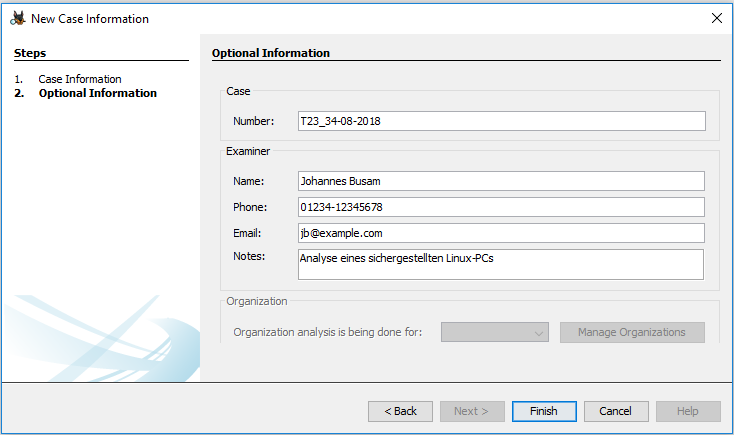
\includegraphics[width=\textwidth]{./resource/autopsy_1_case_information.png}
  \caption{Erstellung eines neuen Falls mit Autopsy}
  \label{fig:autopsy_1_case_information}
\end{figure}

\noindent
Im nächsten Schritt kann dem Fall eine neue Datenquelle hinzugefügt werden. Es werden folgende Typen von Datenquellen unterstützt:
\begin{itemize}
\item Ein Datenträgerabbild im \textit{RAW}-Format, Encase-Format oder ein Abbild einer virtuellen Maschine (z.B. von Virtual Box).
\item Ein lokales Laufwerk (z.B. eine externe Festplatte).
\item Logische Dateien aus einem verfügbaren Dateisystem (z.B. ein beliebiger Ordner).
\item Ein Abbild eines beliebigen Speicherbereiches in einer Datei.
\end{itemize}

\noindent
Im konkreten Fall wird ein Datenträgerabbild als Datenquelle hinzugefügt. Dabei muss auch noch eine Zeitzone angegeben werden. Diese Zeitzone kann entscheidend für die Analyse der Zeitstempel auf einem Datenträger sein. In einem \textit{ext}-Dateisystem bei gängigen Linux-PCs werden die Zeitstempel als Anzahl der Sekunden seit dem 1. Januar 1970 in der Zeitzone \acrshort{utc} gerechnet.\cite[S. 326]{filesystem_forensic}\footnote{Diese Zeitdefinition entspricht der sogenannten Unixzeit.} Bei den älteren \textit{\acrshort{fat}}-Dateisystemen hingegen wird die Zeit ohne Zeitzone gespeichert.\cite[S. 192-194]{filesystem_forensic} Je nachdem in welcher Zeitzone das Betriebssystem konfiguriert wurde, welches die Dateien in dem FAT-Dateisystem änderte, ergeben sich zeitliche Unterschiede. Daher muss bei Zeitstempeln auch später bei der Anzeige der Analyseergebnisse immer auch auf die Zeitzone geachtet werden.\footnote{Ein weiteres interessantes Problem ergibt sich auch bei der Sicherung der Beweismittel an einem Tatort. Auch dort ist nie garantiert, dass alle gesicherten Beweismittel überhaupt zeitlich synchronisiert sind. Gerade in Kombination mit Netzwerkverbindungsdaten können bei einer fehlenden Zeitsynchronisation kritische Abläufe zeitlich versetzt sein. Daher muss gerade die Aussagekraft von Zeitstempel immer kritisch betrachtet werden.}\\

\noindent
Im nächsten Schritt können diverse Module zur Datenaufbereitung aktiviert werden. Diese Module dienen zur automatischen Datenaufbereitung und werden ausführlich in Kapitel \ref{sec:common_analysis_approach_part2} beschrieben. In dem Kapitel erfolgt auch der Vergleich zur der automatisierten Auswertung mit der hier entwickelten Analyseplattform.\\
Nachdem die entsprechenden Module ausgewählt wurden, beginnt Autopsy die Datenquelle zu analysieren. Dies läuft vollständig im Hintergrund ab und der Nutzer kann parallel hierzu die Datenquelle manuell analysieren.\\ 

\noindent
Das Importieren einer Datenquelle bei Autopsy besteht letztlich aus dem Erstellen eines Falls und der Angabe einiger Konfigurationsmöglichkeiten. Die Datenquelle wird hierbei nicht in einen internen Anwendungsordner kopiert, sondern während der Analyse auf dem Rechner bereitgestellt (entweder als Datenträgerabbild oder direkt als externer Datenträger). 
In dem Anwendungsordner von Autopsy werden Metainformationen, wie beispielsweise die Indexierung bestimmter Daten, abgespeichert um während der Analyse schneller darauf zugreifen zu können. Prinzipiell ist dieses Vorgehen sehr gut, da der Ermittler direkt mit der Arbeit beginnen kann und keine Daten kopiert werden müssen.\footnote{Das Erstellen eines Datenträgerabbildes aus dem originalen Asservat wurde hierbei schon vorher durchgeführt.}

\section{Umsetzung in der forensischen Analyseplattform}

Im vorangegangen Kapitel wurde bereits beschrieben, wie Datenträgerabbilder als sogenannte Datenquellen in Autopsy importiert werden. Das Datenträgerabbild oder der extern angeschlossene Datenträger wird nicht in einen internen Anwendungsordner kopiert. Autopsy arbeitet direkt auf den Daten, um ein unnötiges Kopieren von Daten und dessen Ressourcenaufwand zu vermeiden. \\

\noindent
Im Vergleich hierzu arbeitet die hier entwickelte forensische Analyseplattform auf einem eigenen Computer-Cluster basierend auf mehreren Knoten und nicht nur auf einem einzelnen Analyserechner. Daher müssen die forensisch relevanten Daten zuerst über das Netzwerk in die Analyseplattform importiert werden. \\
Da die Analyseplattform auf dem Hadoop-Framework aufbaut, bildet der Kern der Datenspeicherung das \gls{hdfs}.\footnote{Siehe Kapitel \ref{sec:theory_hdfs}.} Hierbei geht es nicht nur darum, wie die Daten im Hadoop-Framework verwaltet werden, sondern vielmehr um die Art und Weise, wie Daten forensisch korrekt gespeichert werden können.\\


\noindent
Zur Speicherung der Daten des Datenträgerabbildes im Hadoop-Framwork gibt es mehrere Möglichkeiten, deren Vor- und Nachteile nachfolgend dargestellt werden sollen.

\section{Variante 1 - Datenträgerabbild im HDFS speichern}
\label{sec:variant1}

Die naheliegende Variante zur Speicherung der Asservate, wäre die Datenträgerabbilder direkt im HDFS abzuspeichern. Allein die Größe der Abbilder ist nicht problematisch. Um eine entsprechende Aufteilung kümmert sich das \gls{hdfs}. Allerdings hat die Lösung den entscheidenden Nachteil, bei der Weiterverarbeitung der Daten.\\ 

\noindent
Auf Betriebssystemebene können solche Datenträger mit mehreren Partitionen und unterschiedlichen Dateisystemen interpretiert und eingebunden werden. Dabei liegen die Dateien als fragmentierte Blöcke in einer spezifischen Datenstruktur vor, welche das Dateisystem des Abbildes beschreiben. Je nachdem, ob ein Datenträgerabbild direkt von einer Partition eines Datenträgers oder vom ganzen Datenträger erstellt wurde, sind in dem Abbild unter Umständen auch mehrere Partitionen samt Partitionstabelle enthalten. 
Von diesen Partitionen kann wiederum jede einzelne Partition ein eigenes Dateisystem, wie zum Beispiel ext4 oder \acrshort{ntfs} enthalten. Dieses Dateisystem enthält die eigentlichen Dateien, welche logisch zusammengesetzt werden müssen. Viele Betriebssysteme bieten hier bereits eine weitreichende Unterstützung zum Lesen und Schreiben dieser Dateisysteme. Hierzu können die Dateisysteme einzelner Partitionen des Datenträgerabbildes \textit{gemountet} werden.\\

\noindent
Innerhalb des Hadoop-Frameworks findet sich jedoch keine Unterstützung zum Lesen von beliebigen Dateisystemen. Denn normalerweise nutzen Java-Applikationen ein definierte Schnittstelle auf Basis von Dateien, die wiederum vom Betriebssystem bereitgestellt werden. Um die logischen Dateien aus dem Datenträgerabbild extrahieren zu können, müsste für jedes einzelnes Dateisystem eine eigene Implementierung in Java geschrieben werden. Diese Implementierung müsste dann auch noch für das HDFS-Dateisystem optimiert sein.\\ 

\noindent
Darüber hinaus wäre das Extrahieren der Dateien aus einem Dateisystem auf einem Datenträgerabbild, gespeichert im \gls{hdfs}, auch nicht performant. Angenommen das Auslesen würde mit Apache Spark durchgeführt werden. Aufgrund der eingangs beschriebenen Datenlokalität (siehe Kapitel \ref{ch:theory_hadoop}) wären auf jedem Knoten einzelne Blöcke von beispielsweise 128 MB Größe vorhanden. Um im ext4-Dateisystem eine Datei lesen zu können, sollten zumindest die Dateisystemmetadaten verfügbar sein. Darüber hinaus kann der Dateiinhalt einer einzelnen Datei verstreut innerhalb des Dateisystems liegen. Je nach Grad der Fragmentierung des Dateisystems, müssten auf einem Data-Node innerhalb des Clusters schlimmstenfalls dutzende weitere Blöcke anderer Knoten nachgeladen werden, um den Inhalt einer einzelnen Datei zu verarbeiten. Dies würde das Prinzip der Datenlokalität aushebeln.\\
Abbildung \ref{fig:ext4_to_hdfs} skizziert diese verstreute Aufteilung einer Datei im physikalischen Hadoop-Cluster.\\ 
\begin{figure}[ht]
  \centering
  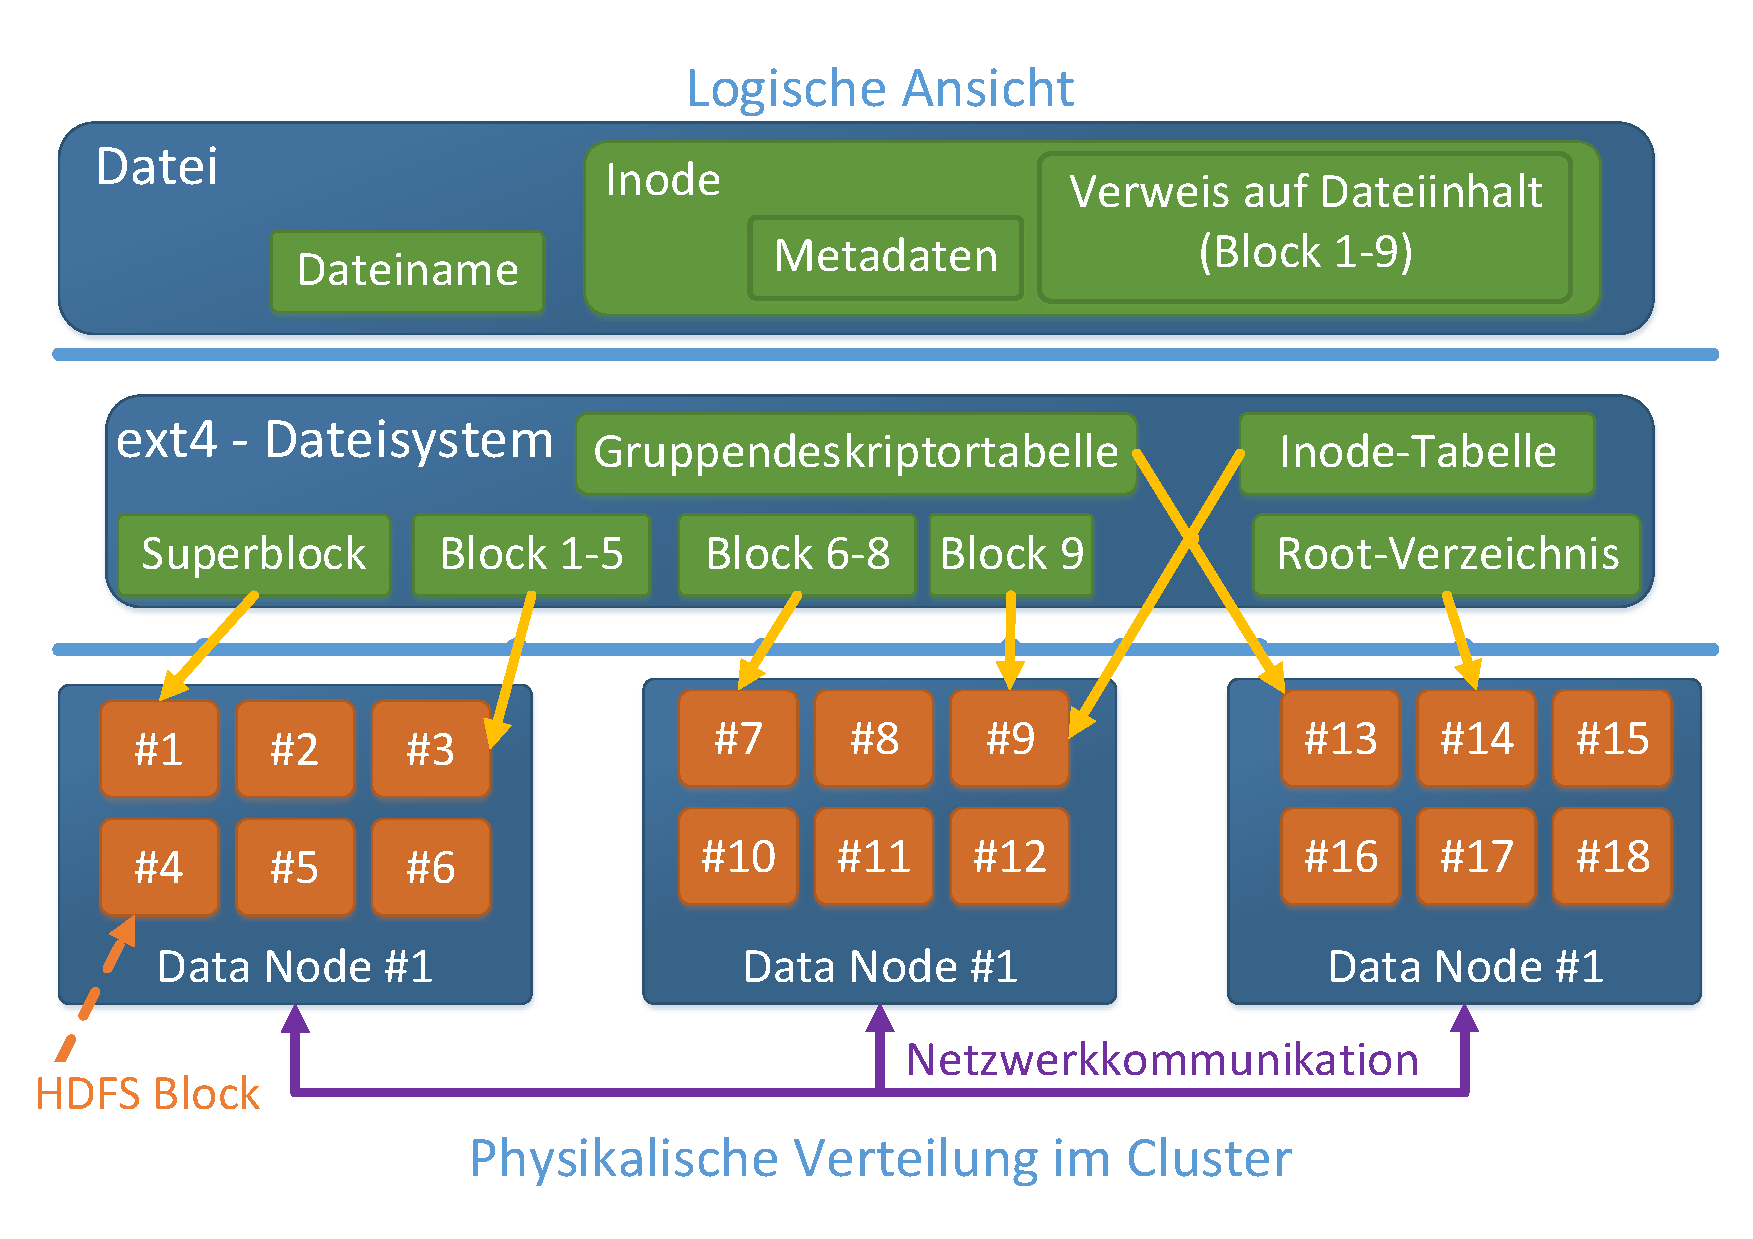
\includegraphics[width=\textwidth]{./resource/ext4_to_hdfs.pdf}
  \caption{Aufteilung der Daten des Datenträgerabbildes im Hadoop-Cluster}
  \label{fig:ext4_to_hdfs}
\end{figure}

\noindent
Das Abbild zeigt eine Datei, welche aus logischer Sicht einen Dateinamen, Metadaten (beispielsweise Zugriffsrechte) und einen Inhalt besitzt. Der Inhalt ist in 9 Blöcke zu jeweils 2048 Byte aufgeteilt.\footnote{Die Blockgröße wird hierbei vom ext4-Dateisystem bestimmt und ist die kleinste allozierbare Einheit im Dateisystem. In der physikalischen Aufteilung im HDFS gibt es auch Blöcke, welche aber eine Größe von 128 MB aufweisen (orange in Abbildung \ref{fig:ext4_to_hdfs}).} Um nun den Inhalt aus dem ext4-Dateisystem einer Datei auszulesen wird zuerst der Superblock benötigt. 
Dieser enthält allgemeine Informationen zum Dateisystem. Darauf wird die Gruppendeskriptortabelle benötigt, um auf einzelne Blockgruppen zuzugreifen.\footnote{Das Dateisystem ist in mehrere autarke Bereiche unterteilt, welche für sich genommen eigenständig Daten einer Teilmenge aller Dateien vorhalten. Dies sind die sogenannten Blockgruppen.} Über eine Blockgruppe kann wiederum auf die Inode-Tabelle zugegriffen werden. 
Diese speichert die Metadaten einzelner Dateien als sogenannte \textit{Inodes} ab. Ein Inode-Eintrag hält wiederum Verweise auf die Blöcke, welche den Dateiinhalt beschreiben. Der Dateiname ist wiederum in dem logisch übergeordneten Verzeichnis gespeichert. Das oberste Verzeichnis ist das Wurzelverzeichnis. Dieses enthält die Namen der Kind-Dateien und entsprechende Verweise zum Inode.\\
Beim Auslesen einer Datei müssen nun etliche Speicherstellen innerhalb des Dateisystems gelesen und interpretiert werden. Angenommen, dass ein konkretes ext4-Dateisystem in einer 100 GB großen Partition gespeichert wird, so wird diese große Datei im HDFS-Dateisystem in 800 große Blöcke zu je 128 MB aufgeteilt und auf den einzelnen Knoten des Clusters gespeichert. 
Hierbei kann aber kein Einfluss darauf genommen werden, wo welche Blöcke mit welchem Inhalt gespeichert werden. Letztlich bedeutet dies wiederum, wenn in einem Apache Spark Executor zu Verarbeitung der Daten eine Datei des Knotens gelesen werden soll, müssen schlimmstenfalls etliche Datenblöcke von anderen Knoten angefordert werden. Dadurch wird auf Netzwerkebene unnötig viel Last erzeugt. Letztlich gilt für das Prinzip der Datenlokalität, dass die einzelnen Blöcke im HDFS möglichst unabhängig voneinander verarbeitet werden können müssen. Diese Problematik trifft übrigens nicht nur bei der Ext-Dateisystemfamilie auf sondern auch bei anderen Dateisystemen.\\

\noindent
Aus den oben genannten Gründen ist die direkte Speicherung von Datenträgerabbilder im HDFS nicht geeignet für die Analyse im Hadoop-Cluster.

\section{Variante 2 - Logische Dateien im HDFS speichern}
In dieser Variante wird das Beweismittel auf dem lokalen Analyserechner gemountet. Darauf aufbauend werden alle Dateien auf logischer Ebene direkt in das HDFS importiert. Damit ist die gesamte Dateisystemstruktur aus dem Datenträgerabbild im HDFS abgelegt. Einzelne Dateien aus dem Datenträgerabbild sind nun auch als einzelne Dateien im HDFS gespeichert und können unabhängig voneinander prozessiert werden. Darüber hinaus ist die Datenstruktur im HDFS unabhängig von dem Dateisystem des importierten Datenträgerabbildes.\\

\noindent
Damit sind die Nachteile der vorangegangen ersten Variante aus Kapitel \ref{sec:variant1} behoben. Allerdings ist das bereits erwähnte File Carving, beziehungsweise das Auffinden von gelöschten Dateien nun nicht mehr im Hadoop-Framework möglich. Denn bei dieser Variante werden ja nur die Dateien aus dem Dateisystem in das Hadoop-Framwork importiert und nicht allokierte Speicherbereiche werden nicht weiter untersucht. Theoretisch wäre es aber auch möglich zusätzlich das vollständige Datenträgerabbild in das HDFS zu importieren, um dann später freie Speicherbereiche analysieren zu können. Im Rahmen dieser Thesis wird diese Einschränkung jedoch vorerst akzeptiert. Eine File Carving ist daher mit der hier entwickelten forensischen Analyseplattform noch nicht möglich. Andererseits können nun in Analogie zur Referenzsoftware Autopsy auch beliebige Verzeichnisse als Datenquelle in die Analyseplattform geladen werden.\footnote{Siehe Kapitel \ref{sec:common_analysis_approach_part1}.}\\ 

\noindent
Interessant an dieser Variante ist das Verhalten des HDFS-Dateisystems bezüglich der Metadaten und der unterschiedlichen Größen von Dateien. Zur Analyse der Dateien auf dem Datenträger werden auch die Metadaten zu den Dateien benötigt. Beim Importieren muss darauf geachtet werden, dass alle Metadaten des lokalen Dateisystems im Datenträgerabbild unverändert in das HDFS kopiert werden. Im HDFS werden auch Metadaten zu den einzelnen Dateien gespeichert. Möglicherweise könnten diese Dateiattribute wiederverwendet werden, um die Metadaten aus dem originalen Dateisystem zu speichern.
Welche Metadaten bereits im HDFS mit angelegt werden, zeigt Abbildung \ref{fig:hdfs_file_properties} anhand eines Ausschnitts aus der Web-Repräsentation eines HDFS.\\
%TODO Abbildung prüfen. Die Darstellung ist zu klein!!! 
\begin{figure}[ht]
  \centering
  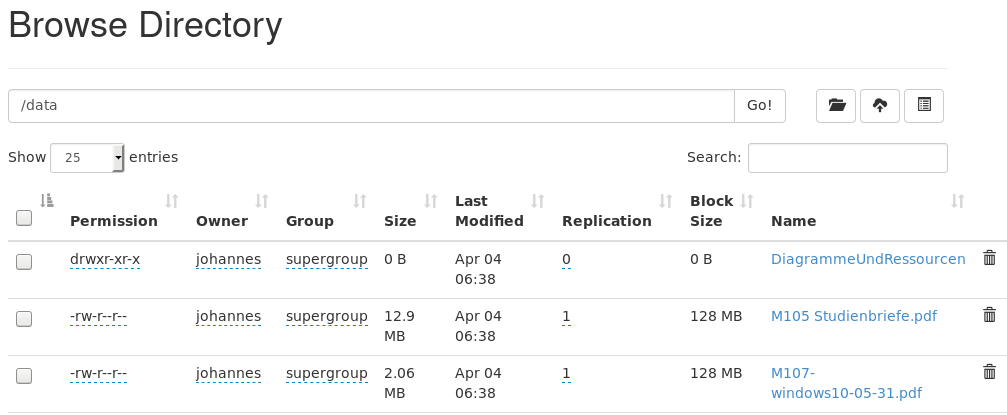
\includegraphics[width=\textwidth]{./resource/HDFS_FS_Example.png}
  \caption{HDFS - Dateieigenschaften}
  \label{fig:hdfs_file_properties}
\end{figure}

\noindent
Daraus ist ersichtlich, dass jede Datei entsprechende Dateirechte hat und einem Nutzer und einer Gruppe zugeordnet ist. Zusätzlich wird die Größe und der Zeitstempel der letzten Änderung gespeichert.\footnote{Bei Dateiverzeichnissen ist die Größe 0 Byte.} Die Anzahl der Replikationen und die Blockgröße sind spezifisch für das HDFS. Jede Datei kann auf einer unterschiedlichen Anzahl von Knoten repliziert sein. Die Standardkonfiguration definiert 3 Replikationen im realen Cluster, wobei Verzeichnisse nur logisch auf dem Name Node abgelegt werden und damit auf keinem DataNode explizit repliziert werden. Auch die Blockgröße ist in der Standardkonfiguration auf 128 MB festgelegt. Wie im Grundlagenkapitel \ref{sec:theory_hdfs} erwähnt, werden die Dateien in mehren Blöcken zu maximal 128 MB gespeichert und auch repliziert.\footnote{Diese Blockgröße kann aber konfiguriert werden.}\\
Bezogen auf klassische Dateisysteme entspricht ein Block im HDFS einem Block im Ext4-Dateisystem oder einem Cluster im NTFS-Dateisystem. Es ist letztlich die kleinste allozierbare Dateneinheit im Dateisystem.\cite[S.129-140]{filesystem_forensic} Dies bedeutet allerdings nicht, dass für jede Datei im HDFS auf den jeweiligen Data Nodes immer mindestens 128 MB Speicher belegt werden. Denn die reale Speicherbelegung auf dem Data Node beschränkt sich auch auf die reale Größe der Datei im lokalen Dateisystem des Data Nodes.\cite[S. 16-17]{professional_hadoop}\\

\noindent
Mit dem Befehl aus Listing \ref{lst:hdfs_put_command} können lokale Dateien in das HDFS importiert werden. 
\begin{lstlisting}[label={lst:hdfs_put_command},caption= Befehl zum Speichern einer Datei im HDFS,captionpos=b,frame=single,style=customshell]
# hdfs dfs -put [source] [destination]
hdfs dfs -put test.pdf /test.pdf
\end{lstlisting}

\noindent
Hierbei werden die ursprünglichen Metadaten der Datei nicht übernommen. So beschreibt der oben erwähnte Modifikationszeitstempel den Zeitpunkt, zu dem die Datei im HDFS das letzte Mal geändert wurde. Dies entspricht initial dem Import-Zeitpunkt. Auch werden Nutzer und Gruppenrechte nicht übernommen. Prinzipiell wäre es aber möglich die Metadaten aus dem lokalen Dateisystem mit in das HDFS zu übernehmen.\footnote{Hierzu kann dem \textit{put}-Befehl aus Listing \ref{lst:hdfs_put_command} der Parameter \textit{-p} mit übergeben werden.} Ratsam ist dies jedoch nicht, da der Nutzer, die Gruppe und die dazugehörigen Zugriffsrechte in einem produktiven HDFS-Cluster verwendet werden, um Zugriffsbeschränkungen einzelner Nutzer und Anwendungen auf Dateien im HDFS umzusetzen. Die Metadaten des originalen Dateisystems sollten daher mit einer anderen Methode im HDFS gespeichert werden.\\

\noindent
Eine bessere Möglichkeit bietet das HDFS mithilfe von erweiterten Dateiattributen. Diese können beliebige Informationen zu einer Datei speichern. Mit nachfolgenden Befehlen kann beispielsweise der Zeitstempel der Erstellung einer Datei aus dem ursprünglichen Dateisystem im HDFS als erweitertes Attribut gespeichert und ausgelesen werden. Hierbei kann der Name des Attributs (\textit{user.ntfs.creationtime}) und dessen Inhalt (\textit{2018-04-07T11:14:42,798583789+02:00}) frei gewählt werden.
\begin{lstlisting}[label={lst:hdfs_fattr_command},caption= Befehl zum Hinzufügen und Auslesen von Metadaten,captionpos=b,frame=single,style=customshell]
# Create custom file attribute
hdfs dfs -setfattr -n user.ntfs.creationtime -v "2018-04-07T11:14:42,798583789+02:00" /test.pdf

# Read custom file attribute
hdfs dfs -getfattr -d -n user.ntfs.creationtime /test.pdf
\end{lstlisting}

\noindent
Mit dem obigen Befehl ist es also prinzipiell möglich, alle Metadaten des ursprünglichen Dateisystems als erweiterte Dateiattribute im HDFS zu speichern. Allerdings müssen diese Metadaten für jede Datei im HDFS eingetragen werden.\\
Zusätzlich müssen beim Verarbeiten der Daten mit Apache Spark die Metadaten auslesbar sein. Dieses Auslesen ist umständlich aber möglich.\footnote{Siehe Metadaten-Extraktion im Projekt \textit{foam-processing-spark} unter \url{https://github.com/jobusam/foam-processing-spark}.}\\

\noindent
Es gibt jedoch zwei entscheidende Nachteile bei dieser Variante, die beide den gleichen Ursprung haben. 
Der erste Nachteil ist, dass jede einzelne Datei aus dem ursprünglichen Dateisystem als getrennte eigenständige Datei in das HDFS hochgeladen werden muss. In einem einzigen Dateisystem können Millionen kleine Dateien gespeichert sein, die alle auch in das HDFS importiert werden müssen. Allerdings ist das HDFS primär für größere Dateien (in der Größenordnung einer Blockgröße von 128 MB) ausgelegt und kann viele kleine Dateien nicht wirklich effizient speichern und bereitstellen. Dies ist dem Umstand geschuldet, dass alle Metadaten auf dem Name Node gespeichert werden und nur der Dateiinhalt im Cluster aufgeteilt wird.\cite[S. 16]{professional_hadoop} Wenn nun viele kleine Dateien gespeichert werden, dann steigt der Speicherverbrauch im NameNode an und beeinträchtigt die Performanz des Systems. Der zweite Nachteil verstärkt dieses Problem. Denn wenn nun auch noch die Metadaten aus dem ursprünglichen Dateisystem als erweiterte Metadatenattribute im HDFS gespeichert werden, dann benötigt der Name Node noch mehr Ressourcen. Darüber hinaus wäre beispielsweise die Verarbeitung der Metadaten mit Apache Spark nur bedingt parallelisierbar, da diese Daten immer zuerst an dem einen Name Node angefordert und über das Netzwerk zu den einzelnen Spark Executoren gesendet werden müssten. Erst dann könnten letztere Executoren die Daten parallel verarbeiten. Abbildung \ref{fig:storage_hdfs_extended_attributes} skizziert nochmals den Datenfluss bei dieser Lösung.\\

\begin{figure}[ht]
  \centering
  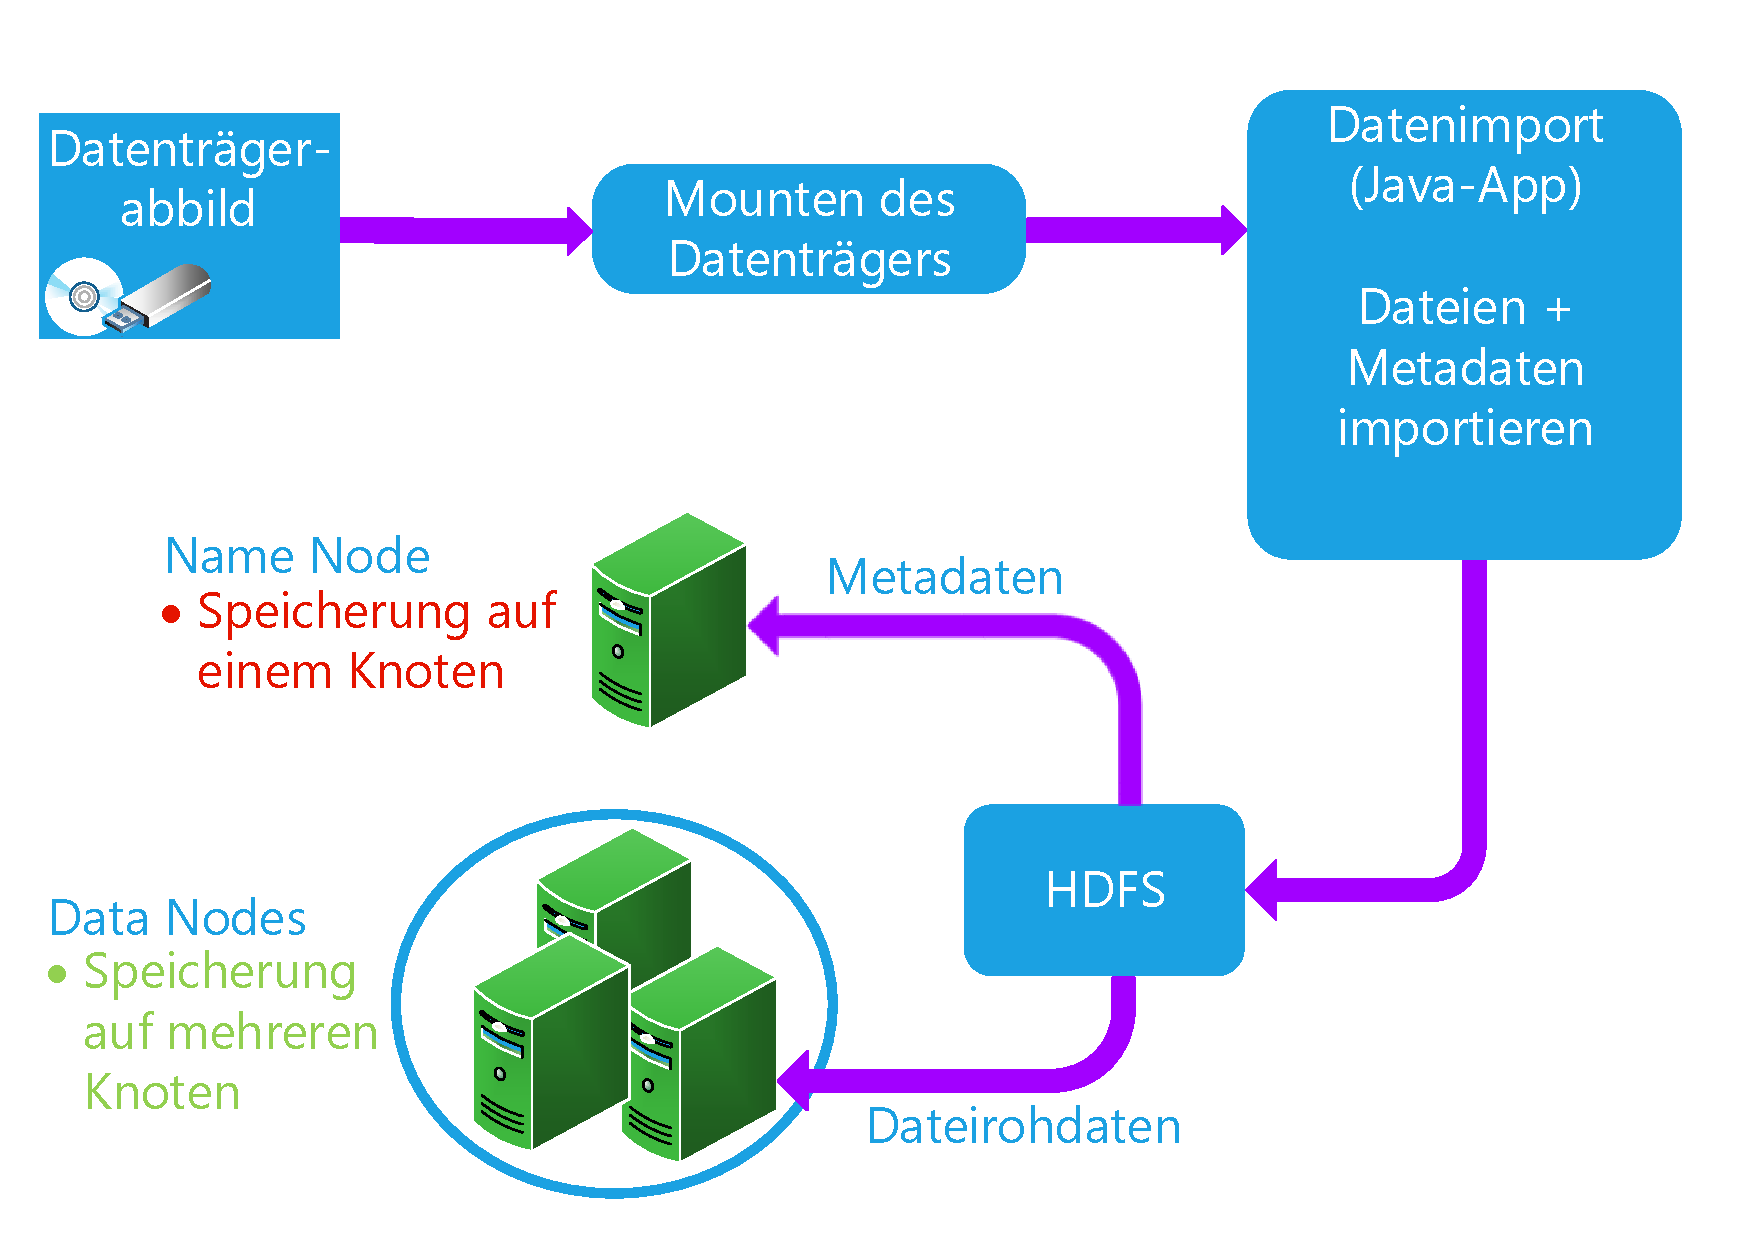
\includegraphics[width=\textwidth]{./resource/storage_hdfs_extended_attributes.pdf}
  \caption{Datenspeicherung mit erweiterten Dateiattributen im HDFS}
  \label{fig:storage_hdfs_extended_attributes}
\end{figure}

\noindent
Das Fazit der Variante 2 lautet daher, dass die Dateimetadaten des originalen Datenträgerabbildes höchstens als erweiterte Attribute im HDFS abgelegt werden könnten. Beim Importieren müssten diese Metadaten bei jeder einzelnen Datei explizit nachgetragen werden. Nicht zuletzt werden alle Datei-Metadaten physikalisch im Name Node gespeichert. Dadurch benötigt der Name Node mehr Speicher und könnte zu einem Flaschenhals im System werden. Zudem wäre die parallelisierte Datenverarbeitung eingeschränkt, da die Metadaten immer zuerst von dem Name Node angefordert werden müssen. Aus diesen Gründen ist die Variante 2 nicht akzeptabel. 

\section{Variante 3 - Speicherung in Dateicontainer}

Die vorangegangene Variante überzeugt nicht, da die Speicherung vieler kleiner Dateien nicht effizient im HDFS durchgeführt werden kann. Da alle Metadaten einer Datei im Name Node abgelegt werden, bildet der Name Node bei vielen kleinen Dateien ein Flaschenhals. Zur Lösung dieser Problematik existieren im Hadoop-Umfeld diverse Dateicontainer. 
Diese Dateicontainer können mehrere Dateien in einem strukturierten Format speichern. In Analogie zu bekannten Dateicontainern, wie beispielsweise \textit{ZIP}-Archiven oder \textit{TAR}-Archiven existieren im Hadoop-Umfeld \textit{Sequence Files}, \textit{\acrshort{rc}/\acrshort{orc} Files}, \textit{Avro-Files} oder \textit{Parquet-Files}.\cite[S. 296]{expert_hadoop_admin} \\
Ziel dieser Dateiformate ist es, viele kleine Daten in größere Dateien zu speichern, um eine bessere Parallelisierung und eine effiziente Speicherung in Hadoop zu ermöglichen. Oftmals unterstützen diese Formate auch eine Datenkompression, um gegebenenfalls Speicherplatz sparen zu können. Viel wichtiger ist jedoch die Teilbarkeit dieser Dateiformate. Wie bereits beschrieben, werden Dateien im HDFS in größere Blöcke geteilt und auf unterschiedlichen Knoten gespeichert. 
Innerhalb eines Blocks muss es also möglich sein, einzelne Einträge beziehungsweise Datensätze lesen zu können. Die oben erwähnten Hadoop Dateiformate unterstützen eben diese Teilbarkeit.\footnote{Im Gegensatz hierzu sind beispielsweise die meisten Dateisysteme in einer Partition eben nicht teilbar. Denn wenn ein Block in der Mitte des Dateisystems ausgelesen werden soll, so können die Daten nicht ohne die Dateisystemmetadaten interpretiert werden. Daher ist auch die erste Variante aus Kapitel \ref{sec:variant1} eben nicht im HDFS anwendbar.}\\

\noindent
Nachfolgend soll das \textit{Sequence File}-Format in Abbildung \ref{fig:sequence_file_format} näher betrachtet werden.\footnote{Siehe auch \cite[S. 134]{hadoop_definitive_guide} und \url{https://hadoop.apache.org/docs/r2.7.5/api/org/apache/hadoop/io/SequenceFile.html}, Stand 18.8.2018.}

\begin{figure}[ht]
  \centering
  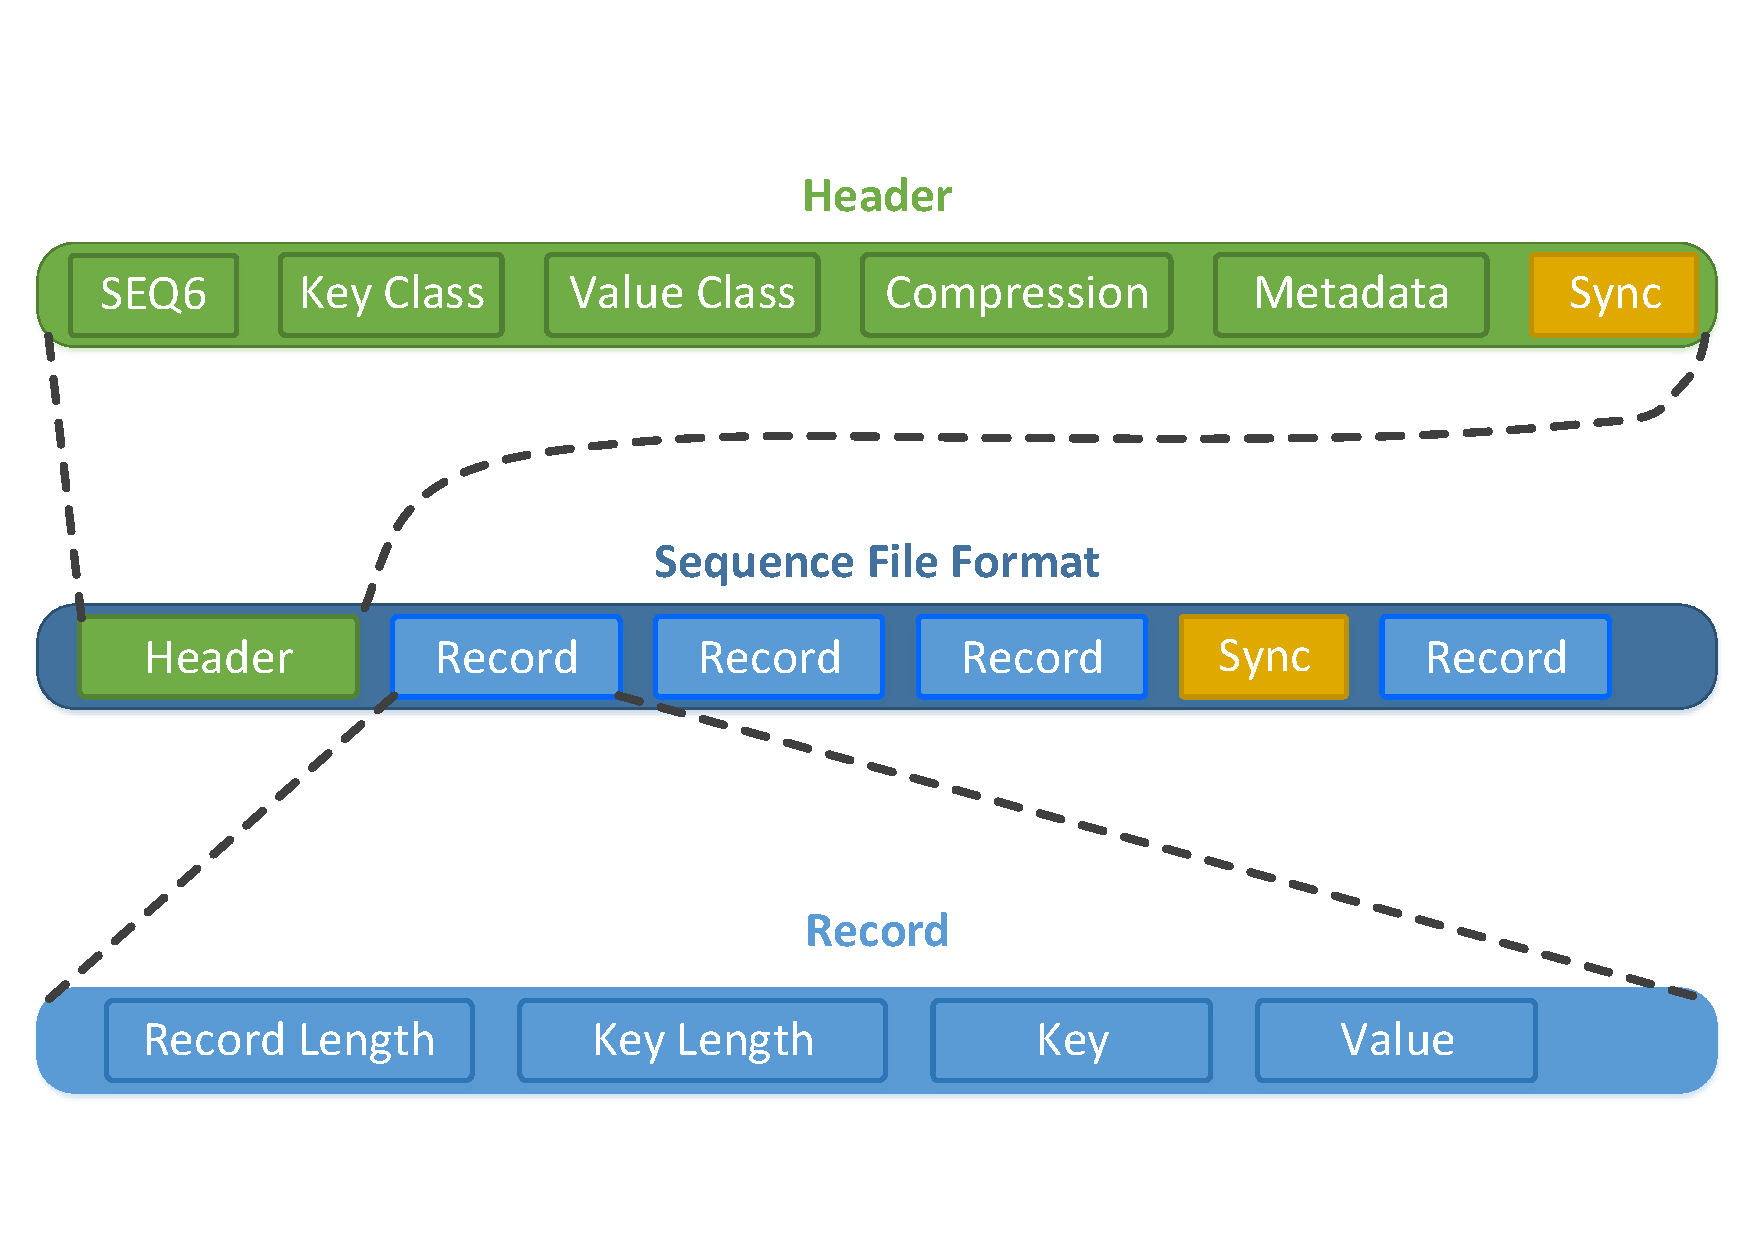
\includegraphics[width=\textwidth]{./resource/sequence_file_format.pdf}
  \caption{Sequence File Format (Vgl. \cite[S. 134]{hadoop_definitive_guide})}
  \label{fig:sequence_file_format}
\end{figure}

\noindent
Das Sequence File Format besteht aus einem Header und mehreren Einträgen. Diese Einträge wiederum sind eigenständige Schlüsselwertpaare, welche die eigentlichen Daten beinhalten. Ein Schlüsselwertpaar, in Abbildung \ref{fig:sequence_file_format} auch \textit{Record} genannt, enthält einen eindeutigen Schlüssel (\textit{Key}) und einen Inhalt (\textit{Value}). Zusätzlich wird am Anfang die Gesamtlänge des Schlüsselwertpaares und die Länge des Schlüssels in Bytes angegeben. Damit ist es möglich den Schlüssel sowie den Inhalt innerhalb des Sequence Files zu bestimmen. Allerdings ist dadurch noch nicht klar, wie der Schlüssel oder Inhalt zu interpretieren ist. Daher sind im Header des Sequence File Formats jeweils die Namen der Java-Klassen in den Feldern \textit{Key Class} und \textit{Value Class} gespeichert, die den Datentyp definieren.  
Im Header befinden sich auch Informationen, ob und in welcher Form eine Datenkompression auf die Daten angewendet wurde.\\
Zuletzt werden in unregelmäßigen Abständen sogenannte Sync-Felder abgespeichert. Diese dienen zur Unterstützung der eingangs erwähnten Teilbarkeit des Dateiformats. Eine Anwendung kann sich mithelfe der Sync-Felder von einer beliebigen Stellen aus innerhalb der Datei auf den Anfang eines Schlüsselwertpaares synchronisieren. Damit können auch Schlüsselwertpaare aus einem beliebigen HDFS-Block interpretiert werden.\footnote{Voraussetzung hierbei ist allerdings, dass die Anwendung vorher schon die Datentypen der Schlüsselwertpaare kennt.}\\ 

\noindent
Prinzipiell können damit sehr kleine Dateien in mehrere Sequence Files strukturiert im HDFS gespeichert werden. Diese Variante enthält aber noch einige Hindernisse. Zuerst stellt sich hier die Frage, wie diese Sequence Files erstellt werden sollen. Hierbei müsste die Anwendung zum Datenimport auf dem Analyse-Rechner die Sequence Files zuerst lokal auf dem Rechner erstellen und danach in das HDFS hochladen. Gegebenenfalls müssten diese Sequence Files sogar noch auf dem lokalen Rechner persistent zwischengespeichert werden. Die Datenimport-Anwendung würde mehr Ressourcen benötigen.\\
Ein interessanteres Problem ist aber die Datenverarbeitung im HDFS. Angenommen es existieren nun Sequence Files mit den Dateiinhalten und den Metadaten in den Dateien. 
Mit Apache Spark können diese Sequence Files gelesen werden und beispielsweise die Hashsummen und die Medientypen ermittelt werden.\footnote{Siehe auch Kapitel \ref{ch:data_processing}.} Allerdings müssten beim Schreiben die Daten in neue Sequence Files geschrieben werden. Denn im HDFS ist es nicht möglich existierende Dateien wahlfrei zu modifizieren.\cite[S. 42]{expert_hadoop_admin} Es können maximal neue Daten an das Dateiende einer Datei geschrieben werden. 
Damit müssten bei der Datenverarbeitung nochmals alle Daten neu geschrieben werden. Dies führt zu unnötigem Ressourcenverbrauch. Andererseits könnten die Rohdaten und die Metadaten in getrennte Sequence Files gespeichert werden. Damit müssten dann nur Sequence Files mit den Metadaten neu geschrieben werden. Es wäre auch denkbar alle neu gewonnen Metadaten in eigenständige neue Sequence Files zu schreiben.\\ 
Allerdings könnte dies wiederum zu einer Art von Fragmentierung von logisch zusammenhängenden Daten führen. Denn nun sind die Metadaten und Rohdaten in mehrere Sequence Files aufgeteilt. Schlimmstenfalls könnten dadurch die Metadaten und Rohdaten, welche eine logische Datei repräsentieren, auf unterschiedlichen Knoten im Hadoop-Cluster liegen. 
Dies würde das Prinzip der Datenlokalität in gewissem Maße beeinträchtigen. Dies hängt aber auch stark davon ab, wie die Daten für die Verarbeitung angefordert werden. Ist es notwendig die Metadaten und die Rohdaten einer logischen Datei gemeinsam zu verarbeiten, oder können diese auch unabhängig voneinander auf getrennten Knoten prozessiert werden?\\

\noindent
Zusammengefasst ist diese Variante technisch möglich. Allerdings besteht eben diese Problematik beim Speichern von neu gewonnen Informationen. Letztlich ist es durchaus sinnvoll wenn die Rohdaten, die originalen Metadaten aus dem ursprünglichen Dateisystem und die neu gewonnenen Metadaten bei der Datenanalyse für eine logische Datei auch physikalisch zusammen gespeichert werden.\footnote{Zumindest sollten die Daten auf dem gleichen Knoten liegen, um Netzwerkverkehr zu vermeiden.}\\ 
Ein anderer Aspekt ist auch die Komplexität der Anwendung. Bei der praktischen Implementierung dieser Variante müsste immer betrachtet werden, wo nun welche Informationen liegen und wie letztlich alle Informationen zu einer Datei aus den Sequence Files zusammengesetzt werden müssen. Dadurch wäre die Implementierung schon sehr komplex. Darüber hinaus sollen ja nur kleine Dateien in Sequence Files abgelegt werden. Große Dateien hingegen könnten ja direkt im HDFS gespeichert werden. Dies würde die Anwendungskomplexität weiter erhöhen. Daher überzeugt auch diese Variante nicht zur Datenspeicherung.\footnote{Die Entscheidung, diese Variante nicht zu verfolgen, basiert nur auf den theoretischen Vorüberlegungen. Auf eine prototypische Implementierung dieser Variante wurde verzichtet, weil mit der vierten Variante zur Datenspeicherung ein Ansatz gefunden wurde, der auch schon in der Theorie mehr überzeugt also die Variante mit Sequence Files.}

\section{Variante 4 - Speicherung mit HBase und HDFS}
Die vorherige Variante beschreibt einen möglichen Ansatz zu Speicherung von kleinen Dateien. Allerdings wurde die Speicherung der Metadaten noch nicht optimal gelöst. Zumal beachtet werden sollte, dass während der Datenverarbeitung weitere Metadaten aus den Rohdaten ermittelt und gespeichert werden.\footnote{Siehe Kapitel \ref{ch:data_processing}.}\\
Da es sich bei den Metadaten um strukturierte Daten handelt, wäre die Speicherung in einer Datenbank naheliegend. Im Hadoop-Umfeld kann hierzu die spaltenorientierte \textit{NoSQL}-Datenbank \textit{Apache HBase} verwendet werden.\footnote{Siehe Kapitel \ref{sec:theory_hbase}.}\\
Auch die Speicherung von kleinen Dateien könnte von HBase übernommen werden. Große Dateien hingegen könnten direkt im HDFS gespeichert werden. 

\subsection{Speicherung kleiner Dateien} 
Diese Problematik von kleinen und großen Dateien wurde bereits in den vorherigen Varianten angesprochen. An dieser Stelle soll diese Thematik nochmals näher betrachtet werden. Nicht zuletzt soll anhand einiger Datenträgeranalysen ein Grenzwert ermittelt werden, nach welchem die Analyseplattform die Dateien entweder in HBase oder im HDFS ablegt.\\

\noindent
Das HDFS kann mit großen und kleinen Dateien umgehen. Die Speicherung großer Dateien ist jedoch der primäre Anwendungsfall. Im Gegensatz dazu können viele kleine Dateien nicht effizient gespeichert werden. 
Es geht aber nicht darum, dass eine einzelne kleine Datei weniger effizient abgespeichert werden kann als eine große Datei. Vielmehr kann der Informationsgehalt einer einzeln großen Datei (beispielsweise als Sequence File) effizienter gespeichert werden, als der gleiche Informationsgehalt aufgeteilt in dutzende kleine Dateien.
Dies liegt daran, dass für jede Datei Metadaten gespeichert werden. Und diese Metadaten werden auf dem Name Node gespeichert und auch im Arbeitsspeicher vorgehalten.\cite{hdfs_architecture} Ein Eintrag ist beispielsweise ungefähr 150 bis 200 Bytes groß. Für eine Datei wird ein Metadateneintrag und ein Blockeintrag im Name Node angelegt (insgesamt 300-400 Byte). Wenn nun ein Million kleine Dateien abgespeichert werden, dann werden 300-400 MB an Arbeitsspeicher benötigt. 
Dies klingt nach einem vertretbarer Ressourcenverbrauch.\\

\noindent
Letztlich geht es aber auch um die Netzwerklast. Denn bei der Verarbeitung der Daten werden auch eine Million Aufrufe an den Name Node gesendet, da nur er weiß, wo der Dateiinhalt liegt. Wenn nun diese eine Million Dateien in ein einzelnes Sequence File gepackt werden, dann benötigt der Name Node nur 300-400 Byte Arbeitsspeicher und zur Datenverarbeitung werden weniger Netzwerkressourcen benötigt.\\

\noindent
Nun stellt sich die Frage, ob eine Million Dateien realistisch anzusehen sind und wie groß kleine Dateien sind. Nachfolgende Abbildungen zeigen hier die Resultate einer Analyse der Dateigröße von diversen Datenträgerabbilder. Abbildung \ref{fig:file_size_c_amount} zeigt hier die kumulierte Häufigkeit der Dateien unterteilt in mehrere Dateikategorien. Diese Kategorien sind logarithmisch nach dem dekadischen Logarithmus aufgeteilt.\footnote{Hierbei wurde die Ergebnismenge der Kategorien linear interpoliert. Der Quellcode zur Berechnung dieser Diagramme wird unter \url{https://github.com/jobusam/foam-data-analysis-ui} bereitgestellt. } Eine Kategorie beschreibt die Anzahl aller Dateien in einem Datenträgerabbild, welche kleiner als die angegebene Kategoriegröße ist. Zum Beispiel existieren auf dem Datenträgerabbild des Windows Systems knapp 400.000 Dateien die kleiner 10 Kilobyte sind.\\

 \begin{figure}[ht]
  \centering
  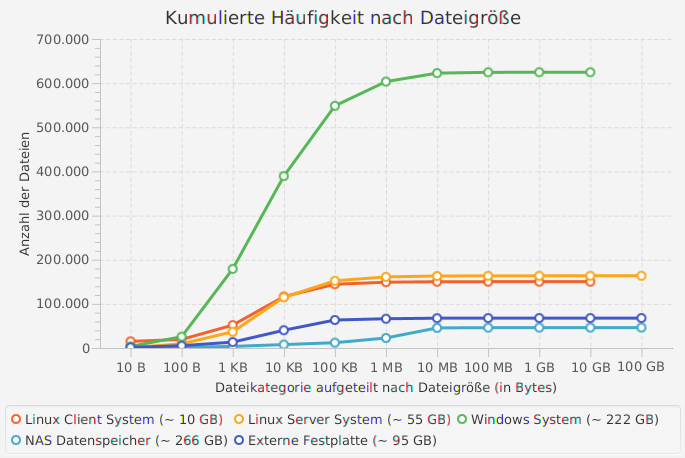
\includegraphics[width=\textwidth]{./resource/fileSize_cumulatedAmount.png}
  \caption{Kumulierte Häufigkeit nach Dateigröße}
  \label{fig:file_size_c_amount}
\end{figure}

\noindent
Nachfolgend werden die Testdaten beschrieben:
\begin{itemize}
\item Das \textit{Linux Client System} ist ungefähr 10 GB\footnote{Die Größenangaben entsprechen den reinen Rohdaten der Dateien. Verzeichnisse und Dateisystemmetadaten sind nicht inkludiert.} groß.\\ Darauf ist ein Ubuntu-Betriebssystem installiert. Es wurde als Testdatenträgerabbild im Rahmen Masterthesis erstellt. Das Abbild enthält 150.229 Dateien.\footnote{Es handelt sich ausschließlich um Datendateien. Verzeichnisse, Symbolische Links und Spezielle Dateien wurden nicht berücksichtigt.}
\item Das \textit{Linux Server System} ist ungefähr 55 GB groß.\\ Darauf ist ein CentOS-Betriebssystem installiert. Das System ist ein Name Node eines kleinen Hadoop-Clusters. Das Abbild enthält 163.555 Dateien.
\item Das \textit{Windows System} ist ungefähr 222 GB groß und ist ein reales Nutzersystem, welches seit mehreren Monaten genutzt wird. Das Abbild enthält 624.650 Dateien.
\item Der \textit{NAS Datenspeicher} entspricht einem QNAP-System mit ungefähr 266 GB an realen Rohdaten. Hierbei ist auf dem Datenträgerabbild kein Betriebssystem installiert. Es handelt sich hauptsächlich um Dokumente und Mediendateien. Das Abbild enthält 46.215 Dateien.
\item Die \textit{Externe Festplatte} mit ungefähre 95 GB Daten, wird als Backup für diverse Mediendateien genutzt. Das Abbild enthält 67.809 Dateien.
\end{itemize}

\noindent
Da die forensische Analyseplattform mehrere Datenträgerabbilder speichern kann, sollte das System durchaus mehrere Millionen Dateien verarbeiten können. Abbildung \ref{fig:file_size_r_c_amount} relativiert die Ergebnisse der einzelnen Abbilder.\\

 \begin{figure}[ht]
  \centering
  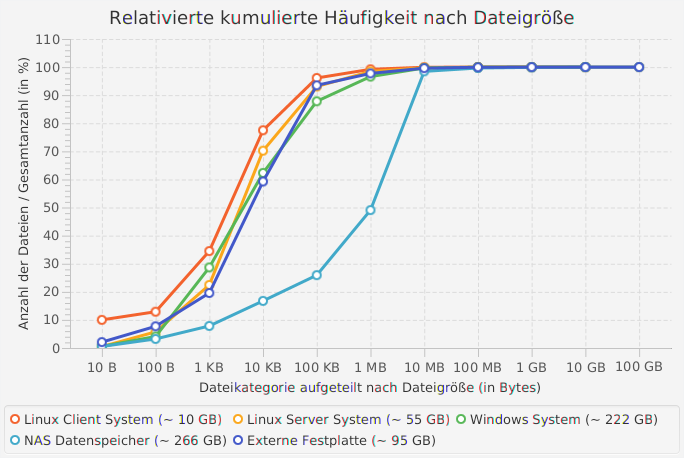
\includegraphics[width=\textwidth]{./resource/fileSize_relativeCumulatedAmount.png}
  \caption{Relativierte kumulierte Häufigkeit nach Dateigröße}
  \label{fig:file_size_r_c_amount}
\end{figure}

\noindent
Anhand der relativierten kumulativen Häufigkeit aus Abbildung \ref{fig:file_size_r_c_amount} wird klar, dass fast 80-90 \% der Dateien kleiner 100 Kilobyte sind und mehr als 95\% der Dateien kleiner 10 Megabyte sind. Allerdings sind diese Angaben mit Vorsicht zu genießen, denn je nach Anwendungsfall können Datenträger beliebige Dateien unterschiedlicher Größe speichern. Ist beispielsweise ein Betriebssystem auf dem Datenträger installiert, existieren allein durch das Betriebssystem tausende von Dateien mit minimaler Dateigröße. Umgekehrt enthält das Datenträgerabbild des \acrshort{nas}-Datenspeichers sehr viele Dateien zwischen 1 und 10 MB. Dies liegt daran, dass von den 46.215 Dateien ungefähr 30.000 Dateien Fotos sind. Diese wiederum sind für gewöhnlich 500 Kilobyte bis 10 Megabyte groß. Die Kurve könnte allerdings anders aussehen, wenn beispielsweise auch Filme und Videos auf dem NAS gespeichert wären.\\

\noindent
Die nachfolgende Abbildung \ref{fig:file_size_c_file_size} und die Abbildung \ref{fig:file_size_r_c_file_size} zeigen die absolute und relativierte kumulative Kategoriegröße der einzelnen Kategorien an. Die Kategoriegröße beschreibt die Gesamtgröße aller Dateien einer spezifischen Kategorie. Beispielsweise sind bei dem Windows System ungefähr 90 Gigabyte der Gesamtdatengröße in Dateien kleiner 10 Megabyte gespeichert.\\  

 \begin{figure}[ht]
  \centering
  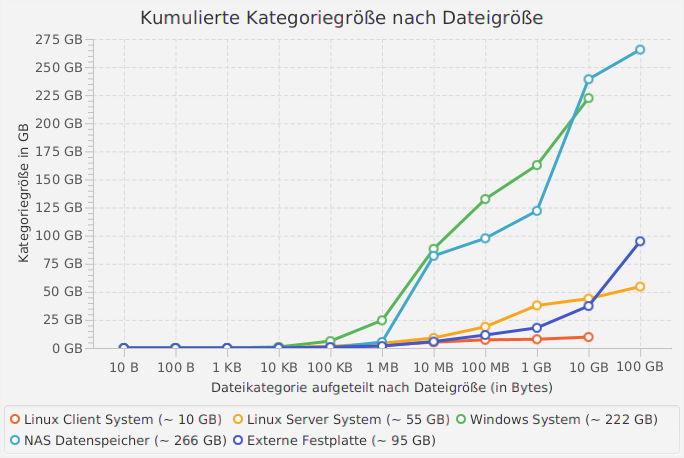
\includegraphics[width=\textwidth]{./resource/fileSize_cumulatedCategorieSize.png}
  \caption{Kumulierte Kategoriegröße nach Dateigröße}
  \label{fig:file_size_c_file_size}
\end{figure}

\noindent
Die relativierte kumulative Kategoriegröße in Abbildung \ref{fig:file_size_r_c_file_size} verdeutlicht den Kontrast in Bezug auf die relativierte kumulative Häufigkeit aus Abbildung \ref{fig:file_size_r_c_amount}. Während mehr als 95\% aller Dateien kleiner 10 Megabyte sind, beansprucht dieser Anteil doch nur ungefähr 10 bis 55 \% der Gesamtspeichergröße.\\

\noindent
Anhand der Diagramme empfiehlt es sich den Grenzwert der Dateigröße zwischen 1 und 10 Megabyte zu definieren. Für die Implementierung im Rahmen der Thesis wird der Grenzwert für die forensische Analyseplattform auf 10 Megabyte gesetzt. Dies bedeutet, dass alle Dateien kleiner 10 Megabyte direkt in HBase gespeichert werden. Darunter fallen beispielsweise auch größtenteils Fotos und Dokumente. Und nur die wenigen großen Dateien (größer 10 Megabyte) werden direkt im HDFS gespeichert.  

%TODO Y-Axis Beschrift ist abgeschnitten
 \begin{figure}[ht]
  \centering
  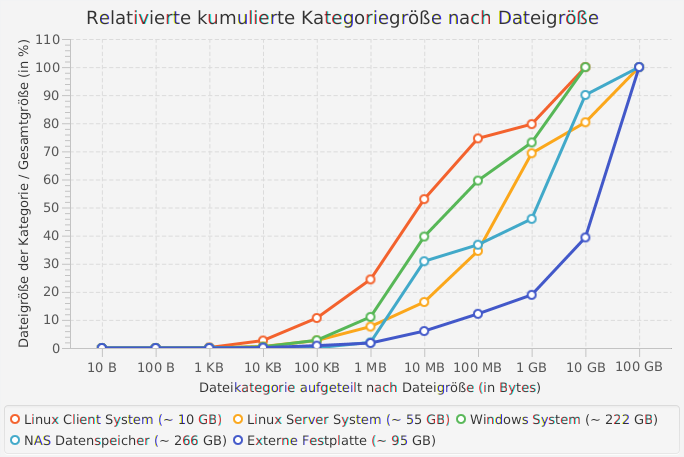
\includegraphics[width=\textwidth]{./resource/fileSize_relativeCumulatedCategorieSize.png}
  \caption{Relativierte kumulierte Kategoriegröße nach Dateigröße}
  \label{fig:file_size_r_c_file_size}
\end{figure}

\subsection{Anwendungsimplementierung} 
\label{subsec:data_import_implementation}

Die Variante zu Datenspeicherung im HDFS-Dateisystem und der HBase-Datenbank wird im Rahmen dieser Thesis implementiert. Das GitHub-Projekt \textit{foam-data-import} enthält diese Anwendung.\footnote{Siehe \url{https://github.com/jobusam/foam-data-import}.} Abbildung \ref{fig:data_import} skizziert die Datenaufbereitung und Speicherung in HBase und im HDFS.\\
\begin{figure}[ht]
  \centering
  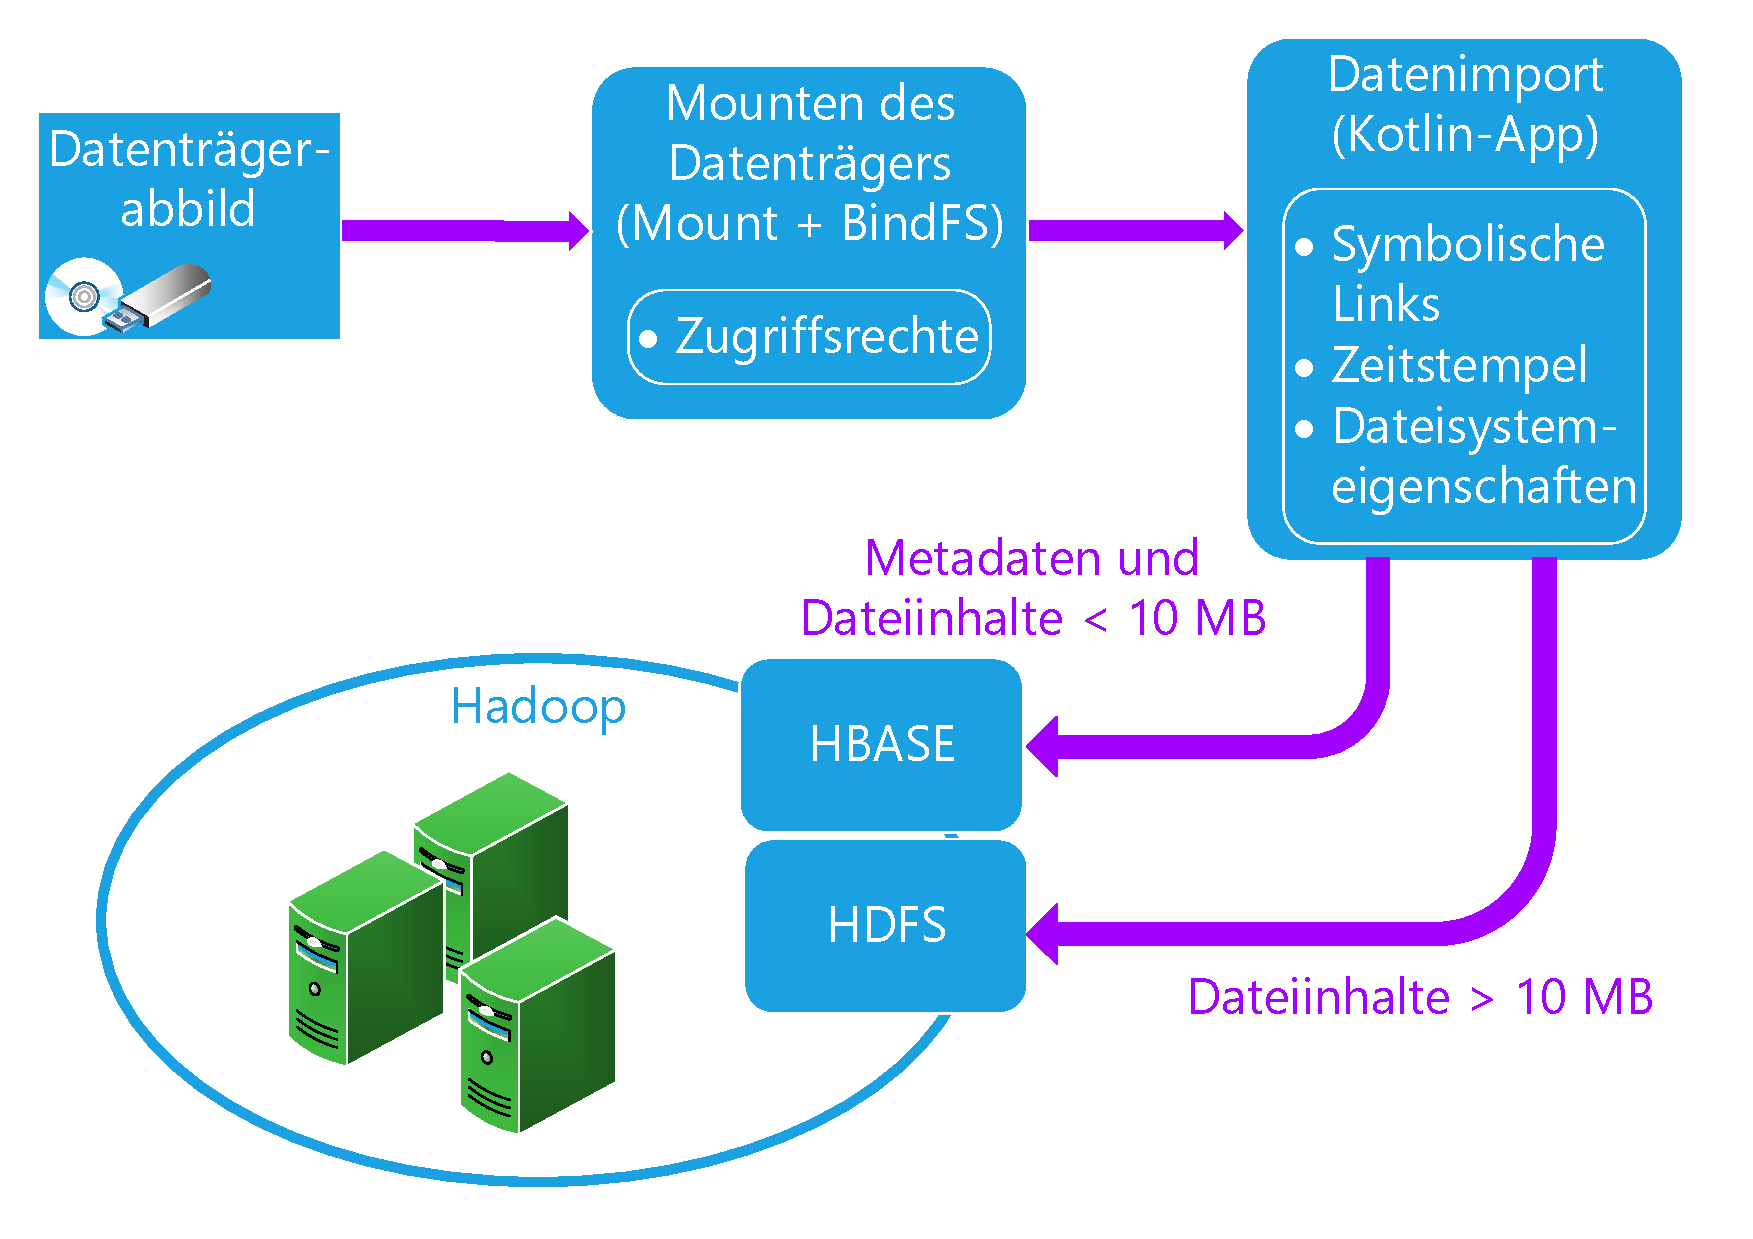
\includegraphics[width=\textwidth]{./resource/storage_hdfs_and_hbase.pdf}
  \caption{Datenimport in HBase und HDFS}
  \label{fig:data_import}
\end{figure}

\noindent
Der Datenimport ist aufgeteilt in zwei Schritte. Der erste Schritt ist das Mounten des Datenträgerabbildes (siehe Abbildung \ref{fig:data_import}). Darüber hinaus müssen die Zugriffsrechte geprüft werden. Die eigentliche Datenimport-Applikation sollte aus sicherheitstechnischen Gründen nicht mit erhöhten Privilegien ausgeführt werden. Daher müssen beim Mounten der Abbilder entsprechende Vorkehrungen getroffen werden. Dieser Vorgang des Mountens muss derzeit manuell mit Betriebssystemwerkzeugen durchgeführt werden. In Kapitel \ref{subsec:data_import_access_rights} wird die detailliert beschrieben, wie die Zugriffsrechte berücksichtigt werden.\\

\noindent
Im zweiten Schritt wird die Datenimport-Anwendung genutzt, um die Daten zu importieren. 
Die Applikation importiert ein vorgegebenes Verzeichnis. Dies kann entweder ein gemountetes Datenträgerabbild sein oder aber auch ein beliebiges logisches Verzeichnis.\footnote{Damit können analog zu Autopsy unterschiedliche Datenquellen importiert werden. Beispielsweise könnte dies ein gemountetes Datenträgerabbild, ein lokaler Datenträger oder einfach nur ein beliebiges Verzeichnis sein. Siehe Kapitel \ref{sec:common_analysis_approach_part1}.} 
Beim Importieren wird jede einzelne Datei des vorgegebenen Verzeichnisses analysiert. Es werden allgemeine Metadaten, wie Name, Größe, Zeitstempel, Zugriffsrechte und Dateityp ermittelt. Das Datenmodell wird detailliert in Kapitel \ref{subsec:data_import_data_model} beschrieben. 
Abhängig von dem Datentyp handelt es sich um ein Verzeichnis, eine Datendatei oder um eine spezielle Datei, wie beispielsweise einen symbolischen Link. Wenn es eine Datendatei ist, dann wird die Dateigröße geprüft. 
Ist die Datendatei größer als 10 MB dann wird sie direkt im HDFS unter einem vorher konfigurierten Dateipfad abgelegt. Ist die Datei kleiner oder gleich groß, dann wird sie zusammen mit den Metadaten in HBase gespeichert.\\
Die Applikation selbst parallelisiert die Metadatenextraktion und den Datenversand über das Netzwerk. Dennoch kann es bei großen Datenträgern durchaus lange dauern, da hier auch die Bandbreite des Netzwerks und vor allem auch die Lesegeschwindigkeit des Datenträgers eine Rolle spielen. 
Befindet sich beispielsweise das zu importierende Verzeichnis auf einem herkömmlichen Festplattenlaufwerk mit Magnetscheiben, ist die Lesegeschwindigkeit und damit auch der Datenimport oftmals um ein Vielfaches geringer als der Import von einer \textit{\gls{ssd}}.\\ 
%TODO Verweis auf die performance tests in einem anderen Kapitel.

\noindent
Die Anwendung wird in \textit{Kotlin} implementiert.\footnote{Siehe auch Kapitel \ref{development_environment} zum allgemeinen Entwicklungsvorgehen.} Diese Sprache wurde zur Entwicklung der Datenimport-App gewählt, um die Vorteile von Java zu nutzen und gleichzeitig neue Sprachkonstrukte verwenden zu können. So ist die entwickelte Applikation interoperabel und kann unter mehreren Betriebssystemen ausgeführt werden. Es muss lediglich ein \textit{\gls{jre}}  installiert sein. Auch die Anbindung zum HDFS und zu HBase kann einfach realisiert werden, da für beide Implementierungen eine Java-Bibliothek bereitsteht. Und letztlich ist es möglich alle benötigten Dateisystemmetadaten auch mit Java und somit mit Kotlin auszulesen. \\
Zum Bauen der Anwendung wird \textit{Gradle} genutzt. Dies ermöglicht eine einfache Handhabung von Third-Party-Bibliotheken und deren Versionierung. Darüber hinaus kann mithilfe von Gradle der Quellcode auch ohne Entwicklungsumgebung schnell und einfach gebaut werden. Somit könnte ein forensischer Ermittler die aktuelle Version aus der Versionsverwaltung unter dem Link \url{https://github.com/jobusam/foam-data-import} herunterladen und mit Gradle bauen.\\
Das Build-Artefakt ist ein Dateiarchiv (ZIP/TAR). Es kann auf einem Analyserechner entpackt und ausgeführt werden. Hierbei wurde der Datenimport als Konsolenanwendung implementiert. Über mehrere Parameter kann der Import konfiguriert werden. Auf eine grafische Oberfläche wurde bewusst verzichtet. Durch die Ausführung als Konsolenanwendung kann das Programm auch sehr gut in andere Analyse-Skripte eingebettet werden.\\

\noindent
Nachfolgende Abbildung \ref{fig:data_import_console_params}  zeigt hier die Hilfeseite und listet alle konfigurierbaren Parameter auf.\footnote{Die Interpretation der Parameter wurde mit der Kotlin-Bibliothek \textit{CLI KT} durchgeführt. Siehe Link: \url{https://ajalt.github.io/clikt/index.html}. Letzter Zugriff: 24.8.2018.}\\
Beschreibung der Parameter:

\begin{itemize}
\item Bei dem Datenimport muss mindestens das Verzeichnis (\textit{Input Directory}) angegeben werden, welches importiert werden soll.
 
\item Mit der Option \textit{-o, -{}-hdfsBaseDirectory} kann angegeben werden, in welches HDFS-Verzeichnis die Dateien größer 10 MB gespeichert werden sollen.\footnote{Hierbei muss der aktuelle Nutzer des Analyserechners auch die Berechtigungen für das Schreiben in das angegebene HDFS-Verzeichnis besitzen.}

\item Die Option \textit{-x, -{}-hbaseSiteXml} gibt den Dateipfad zur Konfiguration von HBase an. Diese Datei kann von einem existierenden Hadoop-Cluster auf den lokalen Analyserechner kopiert werden und definiert eine Gruppe von ZooKeeper-Endpunkten (Hostname inklusive Port), damit über ZooKeeper die HBase-Instanzen ermittelt werden können.\footnote{ In Kapitel \ref{sec:appendix_data_import_config_management} im Anhang wird eine minimale Konfigurationsdatei dargestellt.}

\item Die Option \textit{-y, -{}-hdfsCoreXml} gibt Analog zur HBase-Konfiguration eine HDFS-Konfiguration des Cluster an. Auch hier muss wiederum der Endpunkt zum HDFS angegeben werden.\footnote{Siehe Kapitel \ref{sec:appendix_data_import_config_management} im Anhang.}

\item Mit der Option \textit{-c, -{}-caseNumber} kann eine Fallnummer angegeben werden. Damit können mehrere Asservate zu einem bestimmten Fall zugeordnet werden (siehe Kapitel \ref{subsec:data_import_data_model}).

\item Mit der Option \textit{-d, -{}-caseName} kann zusätzlich ein Fallname angegeben werden.

\item Die Option \textit{-e, -{}-examiner} kann den Namen des forensischen Analysten enthalten. Aktuell muss kein Namen angegeben werden. Allerdings wäre dies später für eine automatische Generierung eines Reports zur Beweismittelkette (\textit{Chain of Custody}) sinnvoll.\footnote{Diese Funktionalität wird im Rahmen der Thesis jedoch nicht implementiert.}

\item Mit der Option \textit{-f, -{}-exhibitname} kann zusätzlich ein Name des Asservats angegeben werden.

\end{itemize}

\begin{figure}[ht]
  \centering
  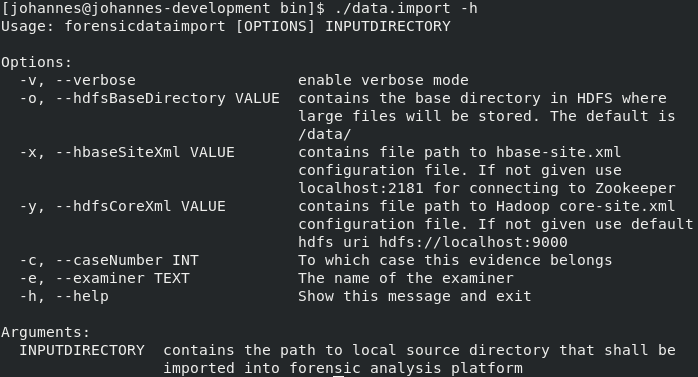
\includegraphics[width=\textwidth]{./resource/data_import_console_command.png}
  \caption{Datenimport-Ausführung in der Konsole}
  \label{fig:data_import_console_params}
\end{figure} 


\subsection{Datenmodell}
\label{subsec:data_import_data_model}

In Abbildung \ref{fig:hbase_data_model} wird das Datenmodell der forensischen Analyseplattform beschrieben. Dieses Modell wird in drei Tabellen in HBase aufgeteilt. 
Es enthält neben der Speicherung der Metadaten auch das Datenmodell einer rudimentären Fallverwaltung.\\

\begin{figure}[ht]
  \centering
  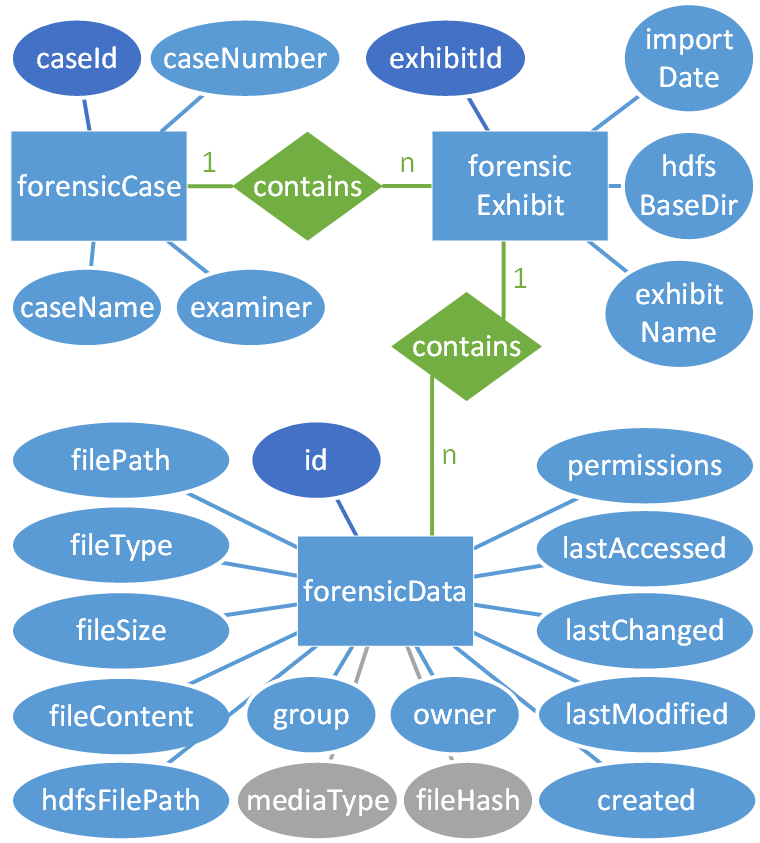
\includegraphics[width=0.8\textwidth]{./resource/hbase_data_model.png}
  \caption{Datenmodell der forensischen Analyseplattform}
  \label{fig:hbase_data_model}
\end{figure}

\noindent
Die Fallverwaltung ist notwendig um den Analysten die Möglichkeit zu geben, mehrere Asservate (z.B. Datenträgerabbilder) in die forensische Analyseplattform zu importieren. Dies ist ein wichtiger Bestandteil um Beziehungen zwischen den Asservaten identifizieren zu können. Ein Fall (\textit{forensicCase}) besteht hierbei aus einer Fallnummer, einem Fallnamen und dem Namen des Auswerters. Die Fallnummer kann beim Datenimport als Parameter angegeben werden. Hierdurch kann der Analyst mehrere Asservate zu einem Fall importieren. Ein Fall kann daher auch mehrere Asservate (\textit{forensicExhibit}) enthalten. Für diese Asservate kann wiederum ein beschreibender Name beim Import angegeben werden. Zusätzlich wird der Zeitpunkt beim Datenimport und das angegebe Basisverzeichnis im HDFS mit abgespeichert. Das Basisverzeichnis wird später bei der Datenverarbeitung ausgewertet, um die Dateien größer 10 MB im HDFS lokalisieren zu können.\\

\noindent
Ein Asservat kann wiederum mehrere Daten (\textit{forensicData}) enthalten. Dies sind die einzelnen Dateien und ihre Metadaten. Hierbei hat jeder Eintrag eine eindeutige Id, welche als Zeilenschlüssel in HBase genutzt wird.\footnote{In Abbildung \ref{fig:hbase_data_model} sind diese Zeilenschlüssel dunkelblau hinterlegt.}. Das Attribut \textit{filePath} enthält hierbei den vollständigen Dateipfad inklusive Dateinamen. 
Im Attribut \textit{fileType} wird gespeichert, ob es sich um eine Datendatei, ein Verzeichnis, einen symbolischen Link und um einer andere spezielle Datei handelt. Abhängig von der Dateigröße wird bei kleinen Dateien der Dateiinhalt direkt in dem Attribut \textit{fileContent} gespeichert. Bei großen Dateien hingegen, wird nur im Attribut \textit{hdfsFilePath} auf den Dateipfad im HDFS referenziert, wo die Datei gespeichert wird. Der Dateipfad im HDFS hingegen ist eine Kombination aus dem angegeben \textit{hdfsBaseDir} und dem Zeilenschlüssel (\textit{id}) des Dateneintrags. Dadurch ist es auch möglich über eine Datendatei im HDFS deren Metadaten in HBase zu identifizieren. Denn der Zeilenschlüssel in der HBase-Tabelle \textit{forensicData} ist innerhalb der forensischen Analyseplattform eindeutig.\\
Des Weiteren werden noch die Zugriffsrechte, die Besitzer, die Gruppe und die Zeitstempel abgespeichert. Je nach spezifischem Dateisystem des Asservats sind allerdings nicht immer alle Metadaten vorhanden.\\
Bei der anschließenden Datenverarbeitung in Kapitel \ref{ch:data_processing} wird das bestehende Datenmodell um neue Metadaten erweitert.\footnote{Hierzu gehören die Attribute \textit{mediaType} und \textit{fileHash}, welche in Abbild \ref{fig:hbase_data_model} grau hinterlegt sind.}

%\noindent
%Ein weitere Punkt ist auch die technische Speicherung. In einem einzelnen HDFS-Verzeichnis können maximal 1048576 Dateien gespeichert werden.\footnote{Siehe Konfiguration von \textit{dfs.namenode.fs-limits.max-directory-items}} Hingegen können in einem lokalen Verzeichnis eines ext4-Dateisystems deutlich mehr Dateien gespeichert werden. Dieser Wert kann maximal auf 6.400.000 gesetzt werden.\footnote{ Siehe \url{https://hadoop.apache.org/docs/r3.0.0/hadoop-project-dist/hadoop-hdfs/hdfs-default.xml} Stand: 23.8.2018.} Wenn ein Dateisystem mehr Dateien in einem Verzeichnis speichert, müsste im HDFS ein zweites Verzeichnis zur Speicherung angelegt werden. Somit ist es auch technisch nicht möglich die gleiche logische Verzeichnisstruktur im HDFS aufzubauen. Bei dieser Variante können bei Bedarf wenigstens neue Verzeichnisse im HDFS angelegt werden! Bei dem Windows-Verzeichnis sind bereits 2000 Dateien größer 10 MB.

%TODO: Siehe HBase MOB (Medium-sized Object Binaries)
\subsection{Datenspezifische Aspekte}
Bei der Implementierung des Datenimports müssen auch datenspezifische Aspekte berücksichtigt werden. Wie bereits erwähnt, werden die Daten auf logischer Dateiebene in das Hadoop-System importiert.
 Hierbei müssen spezielle Dateitypen berücksichtigt werden. Ein Beispiel ist die Verarbeitung von symbolischen Links, welche gerade unter Linux-basierten Betriebssystemen beziehungsweise in der EXT-Dateisystemfamilie auftreten können. Denn wenn symbolische Links in einem Dateisystem gespeichert werden und letzteres im Analysesystem gemountet wird, so können diese Links auch auf Dateien außerhalb des Dateisystems verweisen.
Denn letztlich interpretiert das Betriebssystem diese symbolischen Links. Bei der forensischen Analyse könnte diese  Interpretation aber zu schwerwiegenden Fehlern der Analyseergebnisse führen, wenn Inhalte des Analyserechners verarbeitet werden, welche ursprünglich nicht auf dem Asservat vorhanden waren. Daher muss beim Import geprüft werden, ob die Datei einem symbolischen Link entspricht.
Ist dies der Fall darf, der symbolische Link nur innerhalb des Asservats interpretiert werden.\footnote{Derzeit werden logische Links in das System importiert. Jedoch wird ihre Referenz aktuell beim Import nicht interpretiert. Dies wäre bei einer Weiterentwicklung des Systems durchaus sinnvoll.} \\

\noindent
Auch beim NTFS-Dateisystem, welches vorzugsweise bei Windows genutzt wird, existieren spezielle Eigenschaften. Bei NTFS ist es möglich an Datendateien und sogar an Verzeichnissen sogenannte \textit{Alternate Data Streams} anzuhängen. Diese können, wie jede andere Datei, beliebige Binärdaten enthalten.\footnote{Auch diese Eigenschaften werden im Rahmen dieser Thesis noch nicht beim Datenimport berücksichtigt.}\\

\noindent
Ein weiterer Punkt sind auch die Zeitstempel. Das System kann letztlich die Zeitstempel zur Erstellung einer Datei (\textit{created}), zur letzten Modifikation einer Datei (\textit{lastModified}), zur letzten Modifikation der Metadaten einer Datei (\textit{lastChanged}) und zum letzten Lesezugriff einer Datei (\textit{lastAccessed}) speichern. Letztlich hängt es aber sehr stark von dem genutzten Dateisystem und auch sogar von dem Betriebssystem ab, welche Zeitstempel überhaupt geschrieben werden. Noch kritischer muss die Korrektheit der Daten geprüft werden. Derzeit liest die Datenimport-Anwendung diese Zeitstempel aus, falls sie vorhanden sind.\\

\noindent
Analog zu diesen beschriebenen Fällen gibt es noch weitere dateisystemspezifische Eigenschaften, welche beim Datenimport und zukünftigen Weiterentwicklungen berücksichtigt werden sollten. 

\subsection{Zugriffs und Ausführungsrechte}
\label{subsec:data_import_access_rights}
Ein weiterer Aspekt ist die Beschränkung der Dateizugriffe auf Basis der vorgegebenen Zugriffsrechte. Wie in Abbildung \ref{fig:data_import} in Kapitel \ref{subsec:data_import_implementation} beschrieben wird, muss im ersten Schritt das Datenträgerabbild (beziehungsweise das Asservat) zuerst auf dem Analyserechner gemountet werden. Unter Linux kann dies im Normalfall nur mit erhöhten Administrator-Rechten (root) durchgeführt werden. Der forensische Analyst benötigt also zumindest auf seinem Analyse-Rechner privilegierte Ausführungsrechte. Hier unterscheidet sich beispielsweise die Referenzanalysesoftware \textit{Autopsy} von dieser forensischen Analyseplattform. Denn bei Autopsy unter Windows wird das Dateisystem auf Anwendungsebene direkt mit der Software analysiert. Das Betriebssystem selbst muss das Dateisystem nicht mounten und der Nutzer benötigt daher auch keine besonderen Systemprivilegien.\\

\noindent
Beim Import von Dateien auf einem gemounteten Dateisystem des Datenträgerabbildes sind jedoch die Dateizugriffsrechte weitaus interessanter. Denn das Betriebssystem des Analyse-Rechners berücksichtigt diese Zugriffsrechte. Während diese Problematik bei NTFS-Dateisystemen eine untergeordnete Rolle spielt, so werden hingegen bei ext-Dateisystemen die Unix-Dateirechte gespeichert und auch auf dem Analysesystem interpretiert. 
Daher kann der Nutzer und dessen ausgeführte Programme, welche die Daten aus dem Dateisystem auslesen, nicht in allen Fällen auf alle Dateien zugreifen.\\

\noindent
Die einfachste Möglichkeit um die Problematik der Zugriffsrechte zu umgehen, wäre das Ausführen der Datenimport-Applikation mit Root-Rechten. Andererseits sollte die Applikation nicht mit Root-Rechten ausgestattet werden, da dies im Fehlerfall zu unvorhergesehenen Rechteausweitungen führen könnte und ein Sicherheitsrisiko für die Systemintegrität darstellen würde. Darüber hinaus kann bei einem Fehlverhalten der Anwendung das Analysesystem beschädigt werden. Letztlich braucht die Anwendung zum Datenimport nur die Berechtigungen zum Lesen von Dateien innerhalb des gemounteten Verzeichnisses unabhängig von deren Besitzer und Zugriffsrechten.\\

\noindent
Eigentlich müsste beim Mounten des Dateisystems dem Betriebssystem mitgeteilt werden können, dass die Dateirechte des gemounteten Dateisystems ignoriert werden sollen. Diese Option existiert nicht.\footnote{Zumindest konnte keine funktionierende Variante gefunden werden. Siehe Man-Page des Mount-Befehls (geprüft unter Fedora 28).}\\
Eine weitere Alternative wäre die Möglichkeit mit \glspl{acl} zu arbeiten und dem nichtprivilegiertem Nutzer Rechte zum Lesen der Dateien zu geben. Oder umgekehrt alle Dateien dem nichtprivilegierten Nutzer zuzordnen, welcher wiederum den Datenimport startet.
Hierzu müsste die Datenträgerkopie schreibend gemountet werden, damit die Rechte jeder Datei angepasst werden können. Dies würde wiederum dazu führen, dass das Datenträgerabbild als sichergestelltes Asservat geändert werden würde. 
Daher ist diese Lösung auch nicht geeignet.\\

\noindent
Eine andere Alternative ist die Nutzung von Posix Capabilities\footnote{Siehe Manpages mit folgendem Befehl: \textit{ man 7 capabilities}.}. Dies Variante ist prinzipiell unter CentOS/Fedora möglich. Zum Lesenden Zugriff auf Dateien muss die Posix Capability \textit{CAP\_DAC\_READ\_SEARCH} gesetzt werden.\\
Mit nachfolgenden Kommando kann diese Capability für das Analyseprogramm gesetzt werden.
Damit kann theoretisch auch ein nicht-privilegierter Nutzer lesenden Zugriff auf privilegierte Dateien erhalten.\\ 

\begin{lstlisting}[label={lst:pos_cap_command},caption= Befehl zum Setzen von Posix Capabilities,captionpos=b,frame=single,style=customshell]
setcap CAP_DAC_READ_SEARCH /bin/data.import
\end{lstlisting}
% Mit oder ohne + eip???
%setcap CAP\_DAC\_READ\_SEARCH+eip /bin/ping

\noindent
Allerdings funktioniert diese Alternative primär bei Binärprogrammen, jedoch nicht bei Shell-Skripten oder Java-Anwendungen.\\
Eine ähnliche Alternative zu den Posix Capabilities ist das Setzen des SUID-Bits als Unix-Dateirecht für die Programmdatei. Aber auch diese Möglichkeit funktioniert nur bei Binärprogrammen und nicht für interpretierte Skripte oder Java-Anwendungen, die wiederum in der Java Virtual Machine ausgeführt werden.\\
%Setzen des Flags
%chmod u-s /bin/ping

\noindent
Zuletzt gibt es noch eine Variante, welche die Problematik mit den Dateirechten lösen kann. 
Mit dem Projekt \textit{bindfs}\footnote{Siehe Link: \url{https://bindfs.org/}. Letzter Zugriff: 21.7.2018.} können unter Linux Dateisystemverzeichnisse neu gemountet werden und ihre Zugriffsrechte verändert werden. Der nachfolgende Befehl mountet das existierende Verzeichnis mit den enthaltenen Dateien in einem neuen Verzeichnis und setzt bei jeder Datei die aktuelle ID des Nutzers als Datei-Owner und Group. 
\begin{lstlisting}[label={lst:bindfs_command},caption= Nutzung von Bindfs zum Ändern von Dateirechten,captionpos=b,frame=single,style=customshell]
sudo bindfs -u $(id -u) -g $(id -g) src_dir/ target_dir/
\end{lstlisting}
Der Befehl selbst benötigt Root-Rechte. Jedoch kann der Nutzer danach alle Dateien des Zielverzeichnisses lesen. Das originale Datenträgerabbild wird nicht verändert. Der einzige Nachteil an dieser Lösung ist, dass der Besitzer und die Gruppe jeder einzelnen Datei im neu gemounteten Verzeichnis nun von dem Nutzer des Analysesystems überschrieben wurde.
Dies bedeutet, dass die Attribute \textit{Owner} und \textit{Group} im Datenmodell der forensischen Analyseplattform derzeit nicht korrekt sind und daher auch nicht zur Datenverarbeitung genutzt werden können. Dieser Nachteil muss zukünftig behoben werden, damit die forensische Analyseplattform auch die Besitzer und Gruppen einer Datei korrekt auswerten kann.
Beispielsweise könnte untersucht werden, ob die Implementierung von BindFS modifiziert werden kann, um den ursprünglichen Nutzer und die Gruppe möglicherweise als erweiterte Dateiattribute zu speichern. Diese erweiterten Dateiattribute könnten dann wieder beim Datenimport ausgelesen werden.\\
Alternativ könnte nach weiteren Möglichkeiten gesucht werden, wie dem Betriebssystem
mitgeteilt werden kann, die Dateirechte für bestimmte gemountete Datenträger bei einem lesenden Zugriff zu ignorieren.

%TODO Im Anhang beschreiben, wie bindfs gebaut werden kann.
\section{Fazit} 
Die vierte Variante überzeugt durch eine einfache Lösung zur Speicherung von vielen kleinen und großen Dateien. Darüber hinaus kann mithilfe der HBase-Datenbank auch eine kleine Fallverwaltung implementiert werden, um mehrere Asservate eines Falls zu importieren.\\ Die prototypische Implementierung bestätigt die Machbarkeit zur Speicherung von großen semistrukturierten Datensätzen durch eine Kombination der Speicherung im HDFS und HBase. Aufbauend auf dieser Implementierung und dem dargestellten Datenmodell können im nächsten Schritt der Datenverarbeitung weitere Informationen aus den Daten gewonnen werden. 
\chapter{Datenverarbeitung}
\label{ch:data_processing}

\section{Verarbeitung Apache Spark\texttrademark}
Der physikalische Aufbau wurde bereits im Grundlagenkapitel zu Apach Spark behandelt (siehe Kapitel \ref{sec:theory_spark}). In diesem Kapitel sollen primär die Algorithmen und die Verarbeitung der Daten aus logischer Sicht betrachtet.\\ 

\noindent
Bei Apache Spark gibt es seit der Version 2.0.0 diverse APIs, wie Daten geladen werden können. Es besteht die Möglichkeit Daten mithilfe von Resilient Distributed Datasets (RDDs) zu laden und zu verarbeiten. Aufbauend auf diesen RDDs können, die Daten gemappt, gefilter oder aggregiert werden. Dies Möglichkeit gibt es schon immer in Apache Spark. Seit der Version 2.0.0 gibt es nun auch DataFrames und DataSets (TODO: gibt es beides erst seit v2.0?). Diese Datenstrukturen beschreiben eher eine Schnittstelle aus Sicht von Tabellen. Die Implementierung dieser Typen baut wieder auf den RDDs auf. Doch welche Strukturen eignen sich für die Anwendungsfälle in dieser Thesis? \\

\noindent
DataFrames und DateSets sind optimiert für strukturierte und semi-strukturierte Daten. Diese Daten lassen sich beispielsweise in Tabellenstrukturen einlesen und verarbeiten. Es gibt High-Level Operationen auf diesen Tabellen, welche dem klassischen SQL Syntax sehr nahe kommen?! Apache Spark selbst kann bei der Nutzung von DataFrames und DataSets viele Optimierungen bei der Ausführung und Verarbeitung durchführen. Andererseits sind diese Strukturen ungeeignet bei unstrukturierten Daten, wie beispielsweise Multimediadateien und eben auch beliebigen Dateien.\cite[S. 66 ff.]{data_processing_spark2}\\

\noindent
Wie beim Datenimport schon beschrieben, sind die Metadaten der analysierten Datenträger strukturiert beziehungsweise semi-strukturiert in HBASE abgespeichert. Prinzipiell wäre es also möglich, auch mit Datasets und Dateframes auf diese Daten zuzugreifen. Letztlich kommt es auch auf die Anbindung zwischen Apache Spark und Apache HBASE an. Hierbei gibt es primär zwei unterschiedliche Connectoren\footnote{Bei Apache Spark sind Connectoren eine Art von Java-Bibliotheken, welche es ermöglichen im Apache Spark Ausführungskontext auf andere Systeme, wie beispielsweise Datenbanken oder Dateisysteme, zuzugreifen.}. Der \textit{Hortonworks SHC} Connector ermöglicht die Interaktion mit Daten in HBASE und nutzt dafür die DataFrame/DataSet Datenstrukturen.\footnote{Siehe \url{https://github.com/hortonworks-spark/shc}, Stand: 15.6.2018.} 
Also Pendant auf Basis von RDDs existiert ein weiterer \textit{hbase-spark} Connector. Letzterer wird im Rahmen dieser Thesis genutzt, um Daten von HBASE zu lesen und zu schreiben.\footnote{Siehe \url{https://github.com/apache/hbase/tree/master/hbase-spark}, Stand: 15.6.2018 und deren Nutzung im Projekt \textit{foam-processing-spark} unter \url{https://github.com/jobusam/foam-processing-spark}, Stand: 16.5.2018.}

\subsection{Praxisbeispiele und deren Optimierungen}
Gerade bei der Verarbeitung großer Datenmengen und unter Berücksichtigung des Prinzips der Datenlokalität existieren einige Fallstricke und Hürden bei der Implementierung der Datenverarbeitung. Im Hadoop-Umfeld und bei der Entwicklung im Spark-Context geht es nicht nur um die Art und Weise, wie die Algorithmen auf die Daten angewendet werden, sondern in erster Linie auch immer darum \textbf{wo} die einzelnen Programmteile ausgeführt werden. 
Der Entwickler sollte immer wissen, in welchem Verarbeitungskontext er sich befindet. Zu dieser Problematik werden in diesem Kapitel einige Beispiele herausgegriffen, welche während der Bearbeitung dieser Thesis aufgetreten sind.\\

\noindent
\subsubsection*{Weniger ist mehr TODO}
Ungenutzte Daten so früh wie möglich aus der Verarbeitung rausnehmen. Siehe
Problematik beim HBASE-Spark Connector. Entweder ich mache einen Full-Table Scan und fodere
alle Daten an, um sie später im Spark-Executor auszuführen, oder ich versuche schon beim Zugriff der Daten in den Region-Server mit ColumnFamilies und Filter-Operationen nur die Daten anzufordern, welche auch wirklich benötigt werden. 
\subsubsection*{Caching - Performanz vs. Ressourcen TODO}
Hashing-Problem. Ist es geschickter Daten zu Cachen anstatt sie zweifach anzufordern?
Funktioniert Caching überhaupt mit nicht serializierbaren Daten?
\subsubsection*{Faulheit ist der Schlüssel zum Erfolg TODO}
Lazy-Loading und Ausführung bei RDDs

\subsubsection*{Teile und Herrsche TODO}
Balancing and Repartitionieren. Aufteilung der Last zu gleichen Teilen!
Gerade beim Ausprobieren und Testen ist es einfach, die Resultate eines RDDs nach der Datenverarbeitung über eine Konsole auszugeben. Doch hierbei muss genau überlegt werden, wie diese Resultate ausgegeben werden (siehe Listing \ref{lst:spark_rdd_collect}). In der ersten Variante wird auf dem RDD die Methode collect() aufgerufen und die daraus erhaltene Liste von Objekten wird über ein Logger-Objekt in das Log-File dieser Ausführung geschrieben.\\
Auf der ersten Blick ist aber nicht ersichtlich, was diese Methode wirklich bewirkt. Wie bereits in Kapitel \ref{sec:theory_spark} (TODO: check reference) beschrieben, wird bei der Ausführung einer Spark-Anwendung ein sogenannter Spark-Driver gestartet. Dieser wiederum fordert eine gewisse Anzahl von Exekutoren an, die die eigentlich Datenverarbeitung übernehmen (Master-Slave-Prinzip). Hierbei laufen die Executoren auf einzelnen Knoten innerhalb des Clusters. In dem Moment, in welchem die collect()-Methode auf einem RDD ausgeführt wird, werden die Daten des RDDs \textit{eingesammelt}. Dies bedeutet, dass die Daten des RDDs, welche vorher verteilt auf allen Executoren im Arbeitsspeicher geladen wurden, nun jetzt an den Spark-Driver geschickt werden. Dieser sammelt sozusagen die Ergebnisse der Executoren ein. Diese Mechanismus ist an sich nicht problematisch und funktioniert auch gerade beim Testen mit kleinen Datenmengen. Bei großen RDDs hingegen, werden auch wieder alle Daten an der Driver geschickt und in den meisten Fällen wird dies den begrenzten Arbeitsspeicher des Drivers überfordern. Die Applikation wird mit einer OutOfMemoryException??? beendet!.\\

\noindent
Daher ist es sinnvoll auch schon beim Testen mit kleinen RDDs vorzugsweise die take()-Methode zu nutzen. Diese tut das gleiche wie, die collect()-Methode mit dem Zusatz, dass sie nur ein bestimmte Anzahl von Einträgen sammelt. Dadurch wird selbst bei größeren RDDs der Speicher nicht ausgehen. 


\begin{lstlisting}[label={lst:spark_rdd_collect},caption= Spark Java RDD collect()-Methode ,captionpos=b,frame=single,style=customshell]

HbaseReader hbr = new HbaseReader(jsc, hbaseConfigFile);
JavaRDD<Metadata> forensicMetadata = hbr.getForensicMetadata();

# use collect() method
forensicMetadata.collect().stream()
	.forEach(m -> LOGGER.info("Entry = .", m));

# use take(int amount) method	
forensicMetadata.take(10).stream()
	.forEach(m -> LOGGER.info("Entry = .", m));	
\end{lstlisting}


\section{Anwendungsfälle der Datenverarbeitung}
\subsection{Hashsummen ermitteln}

\subsection{Dateityp erkennen mit Apache Tika}

\subsection{Dateien indizieren}
Ein weitere Anwendungsfall ist die Indizierung von Texten und Wörtern, welche aus den einzelnen Dateien extrahiert wurden.\\

\noindent
Der Grund für eine Indizierung dieser Inhalte ist eine schnellere Suche nach beliebigen Wörtern, als bei der reinen Suche in HBASE. Zur Indizierung existieren zwei bekannte Projekt. Diese sind einerseits \textit{Apache Solr} und andererseits \textit{Elasticsearch}. Bei bauen wiederum auf das \textit{Apache Lucene}-Projekt auf. Apache Solr ist ein Open-Source Projekt unter dem Dach der Apache Foundation. Wohingegen Elasticsearch auch als Open-Source Projekt entwickelt wird, jedoch primär von der kommerziellen Firma \textit{Elastic???} verwaltet wird. Diese bietet gerade Zusatzpakete und Support gegen Bezahlung an.
\subsubsection{Apache Solr}
Spark-Connector von Databracks vorhanden. Der Connector selbst bietet aber vorzugsweise lesenden Zugriff.

\noindent
Abbildung \ref{fig:hbase_solr_indexing} stellt die physikalische Aufteilung mit dem hbase-indexer projekt

\begin{figure}[ht]
  \centering
  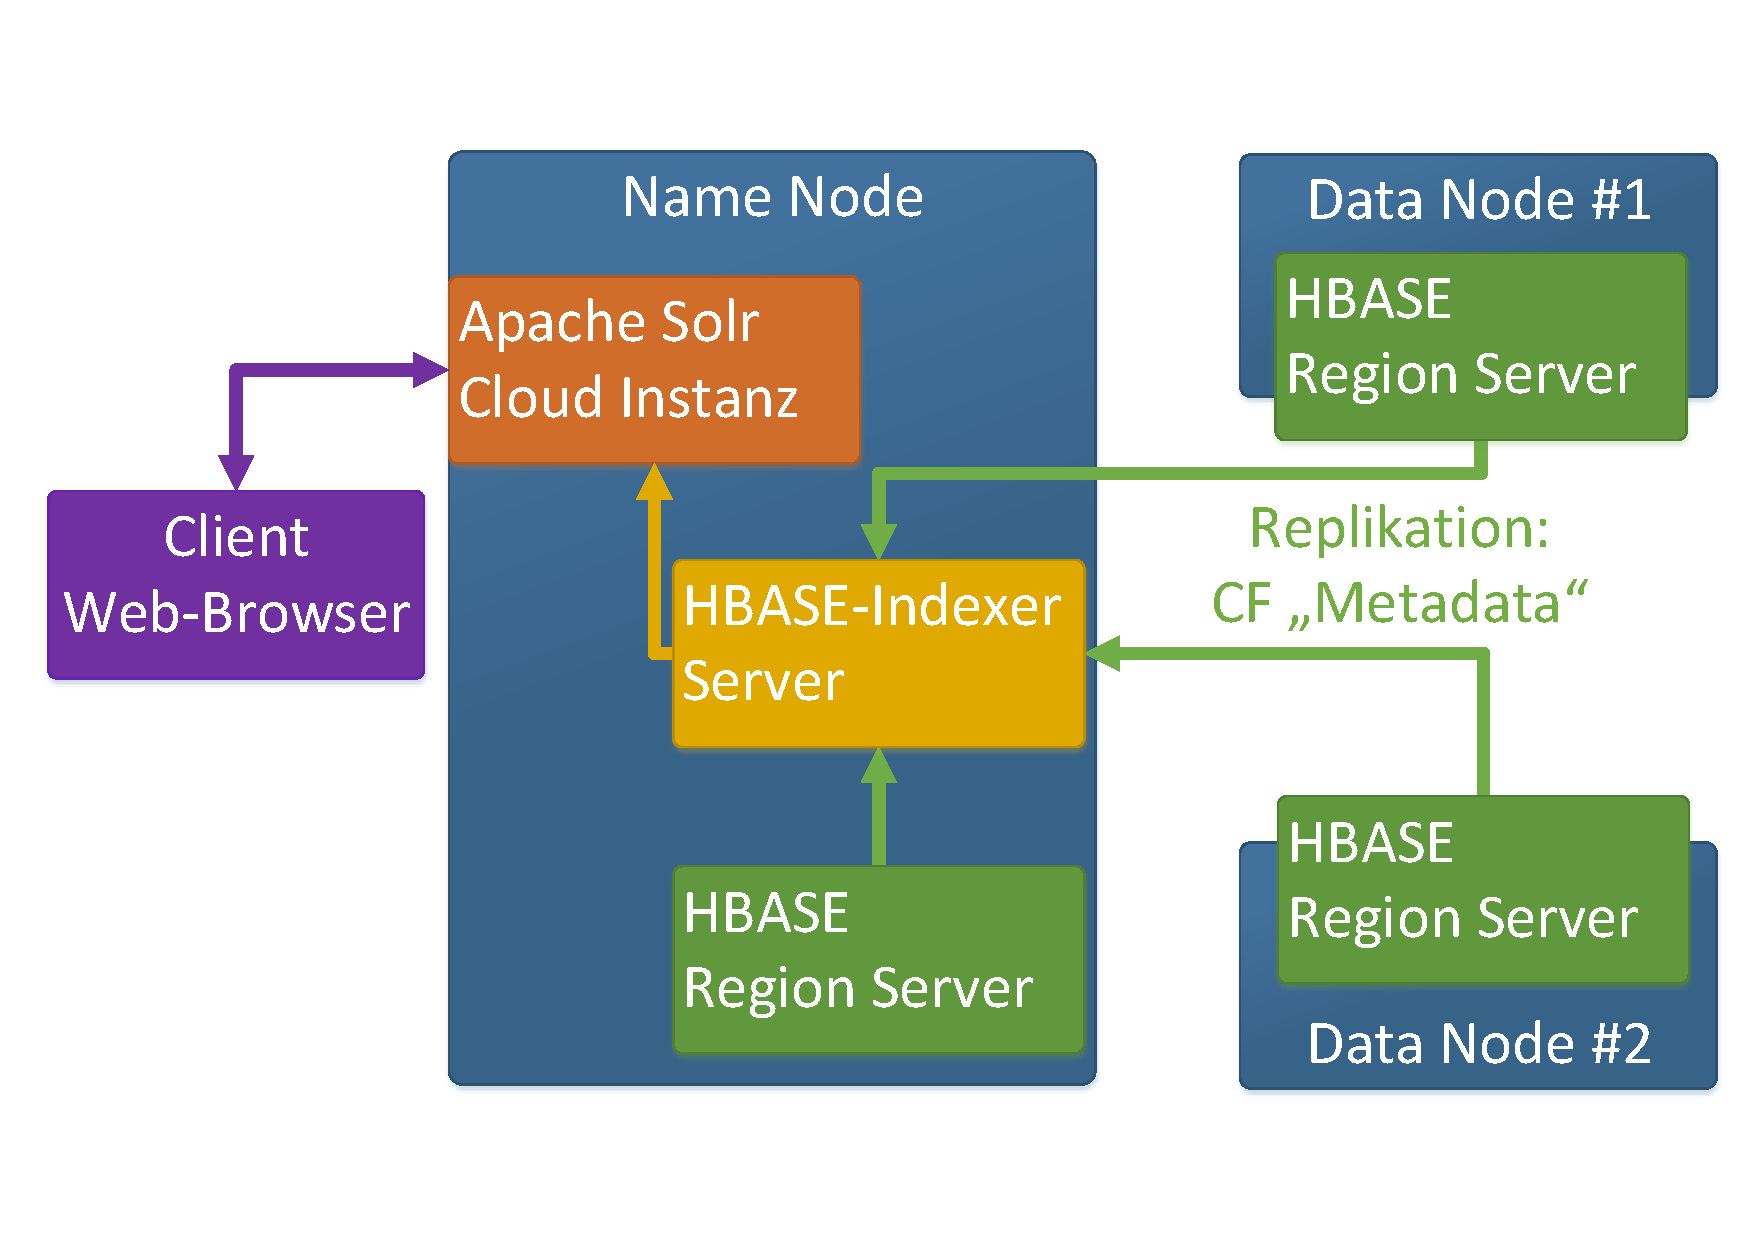
\includegraphics[width=\textwidth]{./resource/hbase_solr_indexierung.pdf}
  \caption{Indexierung von Daten aus HBASE in Solr}
  \label{fig:hbase_solr_indexing}
\end{figure}

\subsubsection{Elasticsearch}
Spark-Connector auf RDD-Basis vorhanden. Kerberos-Sicherung nur über X-Pack gegen Geld vorhanden. Rack-Awareness und Verteilung nicht klar. Elasticsearch baut eigene Infrastruktur auf. Nicht über Ambari steuerbar.
\chapter{Weitere Aspekte}
\label{ch:additional_aspects}

\section{Plattform absichern}
\label{sec:secure_platform}
\subsection{Allgemeines}
Die forensische Analyseplattform muss besonders gegen unbefugten Zugriff gesichert werden, da bei forensischen Analysen unter anderem personenbezogene Daten, aber auch Geschäftsgeheimnisse aus dem kommerziellen Umfeld, verarbeitet werden. Hierbei ist es absolut untragbar, wenn Unbefugte die Daten lesen oder sogar modifizieren könnten.\\

\noindent
Im Hadoop-Umfeld existieren bereits Lösungen, wie Daten vor unbefugtem Zugriff geschützt werden. Das Absichern des Clusters bezieht sich primär auf die Nutzung von Kerberos zur Authentifizierung. Es gibt einige weitere Projekte, wie beispielsweise Apache Ranger, Apache Atlas und Apache Knox, die zum Absichern des Clusters integriert werden können. Sie alle adressieren einen bestimmten Aspekt zur Verbesserung der Systemsicherheit. Nachfolgend soll die Authentifizierung mit Kerberos erklärt werden und Möglichkeiten zur Datenverschlüsselung aufgezeigt werden. Die hier entwickelte forensische Analyseplattform nutzt derzeit weder eine Authentifizierung noch eine Datenverschlüsselung. Allerdings können diese Aspekte in einer zukünftigen Weiterentwicklung implementiert werden.

\subsection{Authentifizierung}

Im Produktivbetrieb wird ein Hadoop-Cluster normalerweise in Kombination mit Kerberos verwendet, um einen allgemeinen Zugriffsschutz zu ermöglichen.\cite{hadoop_security} Nicht nur Apache Hadoop, sondern alle Komponenten aus dem Hadoop-Ökosystem müssen die Nutzung mit Kerberos unterstützen. Bei den hier genutzten Komponenten, wie Apache Spark, Apache HBase und Apache Solr wird daher darauf geachtet, dass sie mit Kerberos arbeiten können.\\

\noindent
Kerberos ist ein kryptografisches Netzwerkprotokoll, welches den Authentifizierungsprozess gegenüber mehreren Servern vereinfachen soll. Dazu werden \textit{Tickets} ausgestellt (\textit{Ticket Single Sign-On}).\cite[S. 425-429]{crypto}\\
Das grundlegende Problem, welches dieses Protokoll löst, ist der erhöhte Verwaltungsaufwand bei der Authentifizierung gegenüber einer Systemlandschaft aus mehreren Servern. Prinzipiell besteht das Hadoop-Cluster aus mehreren Knoten, auf welchen unterschiedliche Services angeboten werden. Bei der forensischen Analyseplattform könnte der Nutzer Daten aus dem HDFS, HBase oder Solr auslesen, eine Datenverarbeitung mit Apache Spark ausführen oder die allgemeine Ressourcenauslastung des Systems anzeigen. Für all diese Aktionen sind unterschiedliche Services und Komponenten verantwortlich. 
Ist das System vollständig abgesichert, müsste sich der Nutzer vor jeder Nutzung bei jedem Service getrennt authentifizieren (beispielsweise mittels Nutzername und Passwort). Darüber hinaus müssten sich auch die Komponenten untereinander authentifizieren, denn Apache Spark greift bei der Datenverarbeitung auf die Daten im HDFS zu und schreibt wiederum Daten in HBase. Um diesen Authentifizierungsaufwand zu verringern, wurde Kerberos entwickelt. 
Bei Kerberos existiert ein zentraler Authentifizierungsserver, gegenüber dem sich ein Nutzer authentifizieren muss. Dieser Server ermöglicht mithilfe sogenannter Tickets die temporäre Authentifizierung gegenüber allen anderen Services, auf welche der Nutzer zugreifen darf.\cite[S. 425-429]{crypto}\\
Abbildung \ref{fig:kerberos} skizziert dieses Verfahren. 
\begin{figure}[ht]
  \centering
  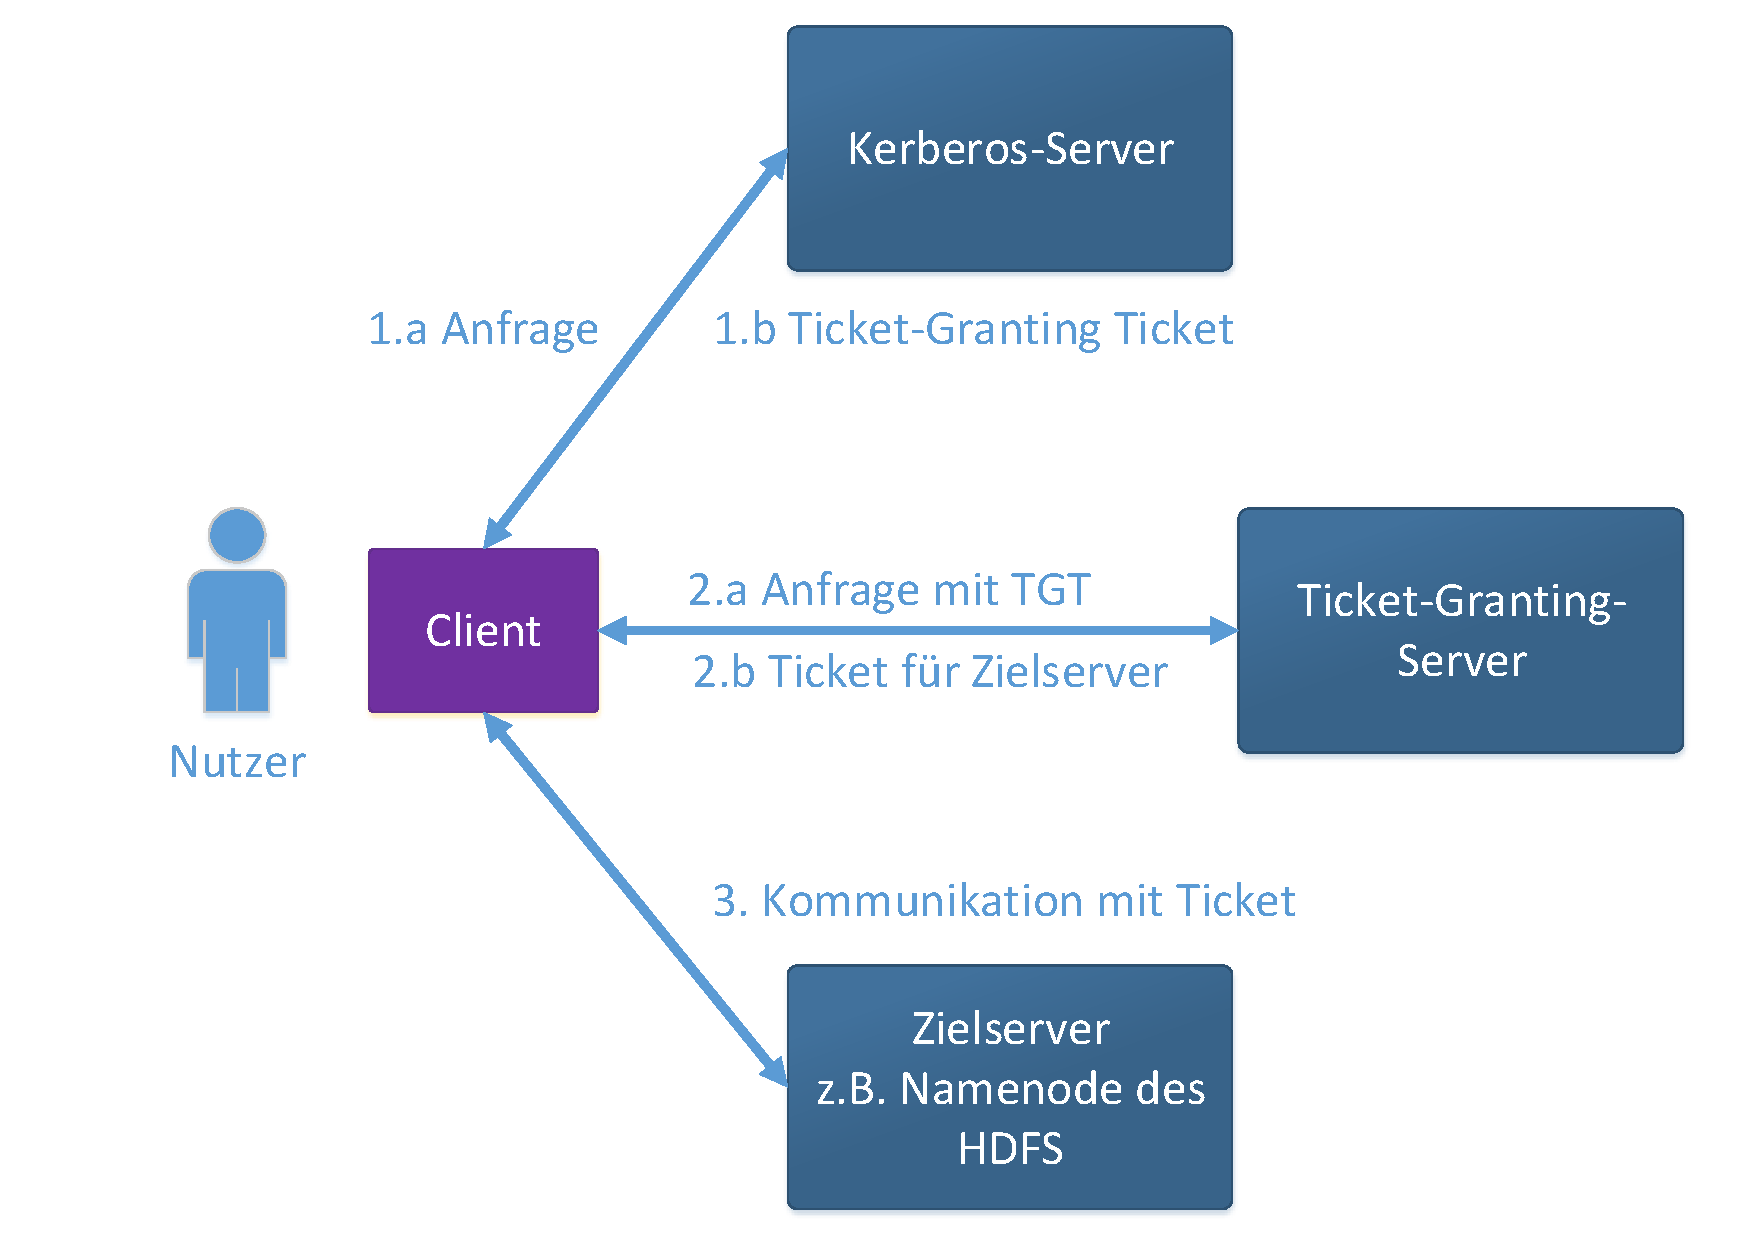
\includegraphics[width=0.9\textwidth]{./resource/kerberos_authentification.pdf}
  \caption{Authentifizierung mit Kerberos (Vgl. \cite[S.426]{crypto})}
  \label{fig:kerberos}
\end{figure}

\noindent
Zu Beginn sendet der Nutzer eine Anfrage an den Kerberos-Server zur Authentifizierung (zum Beispiel mit Nutzername und Passwort). Danach erhält dieser vom Server ein sogenanntes \textit{\gls{tgt}}. Mithilfe des TGT kann er nun beim \gls{tgs} Tickets für spezifische Zielserver und Services anfordern. Mit einem Ticket für einen konkreten Server oder Service kann der Client nun eine verschlüsselte Verbindung mit dem Zielserver öffnen.\\
Ein Ticket ist letztlich ein verschlüsselter Datensatz mit Nutzername und Zugangsberechtigungen für einen spezifischen Server. Der Zielserver kann die für den Server erstellten Tickets vom Ticket-Granting-Server entschlüsseln und so sicherstellen, dass sich der Nutzer authentifiziert hat. Der Ticket-Granting-Server wird bei Kerberos genutzt, um das Schlüsselmanagement sicherer zu machen. Denn dieses Ticket-Granting Ticket ist nur für eine begrenzte Zeit gültig und muss dann wieder neu angefordert werden. Hierdurch ist es für einen Angreifer schwerer, dauerhaften Zugriff auf die Services zu erhalten, falls dieser den Sitzungsschlüssel des Ticket-Granting Tickets ermitteln kann.\cite[S. 425-429]{crypto}\\

%Eine Alternative könnte hier auch Cloudera Sentry, Apache Ranger, Apache Atlas oder Apache Knox\footnote{https://knox.apache.org/} sein.

\subsection{Datenverschlüsselung}
Zum Schutz der Daten im Hadoop-Cluster können diese verschlüsselt werden. Hierbei wird zwischen der \textit{Persistenzverschlüsselung} und der \textit{Transportverschlüsselung} unterschieden. Die Persistenzverschlüsselung kann auf unterschiedlicher Ebene durchgeführt werden. 
Es ist möglich, die Festplatten aller Knoten im Hadoop-Cluster auf Betriebssystemebene zu verschlüsseln. Dabei kann das sogenannte \textit{\gls{luks}} auf Linux-basierten Betriebssystemen genutzt werden, um alle gespeicherten Daten zu verschlüsseln. Diese Art der Verschlüsselung ist unabhängig vom Hadoop-Ökosystem und sichert daher alle Daten auf den Knoten. Allerdings ist die Verwaltung aufwendig, da beim Ersetzen von Festplatten oder dem Hinzufügen neuer Knoten die Verschlüsselung nochmals durchgeführt werden muss. Darüber hinaus werden bei einem Neustart der Knoten die Passwörter zur Entschlüsselung benötigt. Hierzu gibt es spezifische Komponenten, die die Verwaltung der Schlüssel übernehmen. \cite[S. 202-204]{hadoop_security}\\

\noindent
Ein anderer Ansatz ist die Verschlüsselung der Daten auf Applikationsebene. Beim HDFS besteht die Möglichkeit, sogenannte \textit{Verschlüsselungszonen (Encryption Zones)} zu nutzen. Dabei werden schon auf Anwendungsebene die Daten verschlüsselt im HDFS abgelegt. 
Darüber hinaus werden durch die Nutzung mehrerer Verschlüsselungszonen, die Daten innerhalb des HDFS nochmals gegen ungewollte Nutzerzugriffe gesichert. Dies kann beispielsweise die Sicherheit bei der Speicherung von Daten unterschiedlicher Firmen im gleichen HDFS erhöhen. Um die Daten zu entschlüsseln, wird bei dieser Variante ein unabhängiger Schlüsselserver benötigt, der einem Nutzer die entsprechenden Schlüssel abhängig von seinen Zugangsberechtigungen bereitstellt. Zusätzlich existiert ein sogenannter \textit{Hadoop Key Management Server}, welcher die Kommunikation zwischen Client, HDFS und Schlüsselserver steuert.\cite[S. 192-200]{hadoop_security}\\
Diese Variante zur Datenverschlüsselung bezieht sich allerdings nur auf das HDFS. Bei der Datenverarbeitung im Hadoop-Umfeld können die Daten aber auch temporär zwischengespeichert werden. Diese werden nicht von der Datenverschlüsselung im HDFS abgedeckt und sind ungeschützt auf den einzelnen Knoten im Cluster gespeichert. Hier zeigt sich, dass die Absicherung im Hadoop-Cluster immer auch spezifisch für die genutzten Komponenten geprüft werden muss. \\

\noindent
Auch die Transportverschlüsselung im Hadoop-Cluster sollte betrachtet werden, da hier einerseits sensible Daten zwischen den Knoten aber auch von einzelnen Knoten zu den Rechnern der Nutzer transportiert werden müssen. Bei Webservices über HTTP sollte daher die Verschlüsselung mittels \textit{\gls{tls}} durchgeführt werden. Darüber hinaus bietet Apache Hadoop weitere Möglichkeiten, um auch die Kommunikation zwischen den Knoten entsprechend zu verschlüsseln. Auch hier reicht es nicht aus, nur Apache Hadoop zu betrachten, sondern auch alle anderen Komponenten, die im Hadoop-Cluster arbeiten. \cite[S. 207-216]{hadoop_security}\\

\noindent
In der aktuellen Analyseplattform wird derzeit keine Datenverschlüsselung oder Transportverschlüsselung eingesetzt. Zumindest die Transportverschlüsselung sollte in einer zukünftigen Weiterentwicklung implementiert werden, um die Datensicherheit im Netzwerk zu erhöhen.

\section{Datenlöschung}
Das forensisch korrekte Löschen von Daten muss auch im Hadoop-Umfeld betrachtet werden. Bei einer forensischen Analyse werden die Asservate sichergestellt und für einige Zeit verwahrt. Die Computersysteme, mit welchen die Daten analysiert und verarbeitet werden, müssen bereinigt werden. Diese Bereinigung wird meistens durch das mehrmalige Überschreiben der persistenten Datenträger gewährleistet.\\
 Im Hadoop-Umfeld ist dieses Vorgehen aufwendiger. Es ist zwar möglich, mit der hier entwickelten Datenimport-Anwendung aus Kapitel \ref{subsec:data_import_implementation}, die Daten aus dem HDFS und HBase zu löschen. Allerdings bedeutet dies nicht, dass sich danach keine Datenrückstände mehr auf den Festplatten der einzelnen Knoten befinden.
Für gewöhnlich werden die Daten im HDFS über einen längeren Zeitraum gespeichert und müssen nicht forensisch korrekt gelöscht werden. Daher ist es nachvollziehbar, dass im Hadoop-Ökosystem dieser Aspekt bisher nicht ernsthaft betrachtet wurde.\\

\noindent
Das Projekt \textit{\gls{sdhdfs}} versucht, diesen Aspekt zu berücksichtigen und implementiert einen eigenen Mechanismus zum Löschen von Daten im HDFS.\cite{sd_hdfs} Hierbei werden die allokierten Datenblöcke im HDFS auf den einzelnen Knoten überwacht. Die Datenblöcke, welche aus dem HDFS gelöscht wurden, werden mehrmals mit zufällig generierten Daten überschrieben.\\ 
Allerdings ist es fraglich, ob dieser Ansatz wirklich funktioniert. Denn je nach konkretem Speichertyp, ist durch das bloße Überschreiben auf Betriebssystemebene nicht gewährleistet, dass die Daten auch wirklich auf der Festplatte überschrieben werden. 
Dies ist zum Beispiel bei SSDs relevant, da dort der Speicher-Controller selbst entscheidet, in welchen Speicherblock neue Daten geschrieben werden.\\ 
Des Weiteren werden die Daten im Hadoop-Umfeld nicht ausschließlich im HDFS abgespeichert. Beispielsweise könnten Teile der Metadaten in Log-Dateien enthalten sein oder in temporären Dateien zwischengespeichert werden. 
So können bei Apache Spark nach Bedarf auch Zwischenergebnisse persistent auf die Festplatte ausgelagert werden.\cite{spark_rdd} Diese Daten werden bei dem Ansatz von SD-HDFS nicht berücksichtigt. Darüber hinaus wird dieses Projekt nicht mehr weiter verfolgt, da kaum Informationen zu dessen Einsatz bekannt sind.\\

\noindent
Die  derzeit einzige forensisch korrekte Lösung ist die vollständige Datenlöschung aller genutzten Datenträger innerhalb des Clusters. Dies hat jedoch auch die Neuinstallation des Analysesystems auf allen Knoten zur Folge. Aber nur dadurch kann sichergestellt werden, dass temporäre Datenfragmente gelöscht sind.  
\section{Visualisierung der Ergebnisse}
Ziel dieser forensischen Analyseplattform ist es, dem Nutzer einen Überblick bei der Datensichtung zu geben. Hierbei ist es essentiell entsprechende Visualisierungen zu verwenden.
Welche Ziele sollen erreicht werden?
\begin{itemize}
\item Für jede Datei sollen Name, Pfad, Größe,Hashsumme, Dateityp, Owner und Group, Zugriffsrechte und die Zeitstempel der Erstellung und letzter Speicherung angezeigt werden. 
\item Nach all diesen Parametern kann auch gesucht werden.
\item Auffinden von Duplikaten anhand der Hashsummen
\item Indizierung für schnelle textbasierte Inhaltssuche?
\item Zeitleiste? (wohl eher optional)
\item Wordcloud, geographische Visualisierung, Flare-Chart, Tree-Map, Calendar-Chart als Timeline?
\item Webframeworks wie \url{https://d3js.org/} \footnote{Siehe auch \url{https://bl.ocks.org/mbostock/4063550} oder \url{https://bl.ocks.org/mbostock/5944371} oder \url{https://bl.ocks.org/mbostock/1046712} oder \url{https://bl.ocks.org/mbostock/4063269}. Letzteres wäre characteristisch für foAm. oder \url{http://xliberation.com/googlecharts/d3concept.html}}
\item Neo4j
\item Open Source Community Variante Helical Insight
\item Apache Superset für Visualisierung (siehe Ambari Cluster Services)
\item Apache Grafana?
\end{itemize}

\chapter{Diskussion der Ergebnisse}
\label{ch:result_discussion}

TODO: Ergebnisse kritisch betrachten und entsprechende Nachteile aufzeigen.
\begin{itemize}
\item Datenimport dauert lange. Währenddessen können noch keine Daten analysiert werden. Ist Data Streaming eine Alternative? (Siehe Ausblick)
\item Probleme mit den Zugriffsrechten beim Mounten der Datenträger
\item Arbeite das Hadoop-Framework überhaupt effizient?
\end{itemize}
\chapter{Zusammenfassung}
\label{ch:zusammenfassung}
\textbf{TODO: 2 Seiten Zusammenfassung}!\\
%TODO Die Ergenbnisse kurz kritisch hinterfragen und Antworten ob die Plattform für forensische Analysen passen würde. Hier könnte gesagt werden, dass es zwar noch etliche Aspekte fehlen, aber es durchaus mit Hadoop möglich ist!!!

Die Ergebnisse dieser Arbeit zeigen die Machbarkeit einer forensischen Auswertung von großen Datenmengen in einem Computer-Cluster auf Basis von Apache Hadoop. Um die Daten parallel zu verarbeiten, müssen diese in voneinander unabhängig verarbeitbaren Strukturen gespeichert werden. Hierzu bietet es sich an, die Daten als getrennte logische Dateien abzuspeichern, so wie sie aus logischer Sicht in den Datenträgerabbildern persistiert sind.\\
Ein kritischer Aspekt ist die Speicherung beliebig kleiner und großer Dateien für eine optimale Verarbeitung. Als Lösung werden die Vorteile unterschiedlicher Datenhaltungen kombiniert. So werden beliebig große Dateien direkt im verteilten Dateisystem von Apache Hadoop gespeichert. Kleine Dateien, kleiner 10 Megabyte, werden hingegen in der verteilten spaltenorientierten Datenbank HBASE gespeichert. Dort können auch die Metadaten und Analyseergebnisse der Datenverarbeitung abgelegt werden.\\

\noindent
Als Beispiele zur Datenverarbeitung wird die Berechnung von Hashsummen und das Ermitteln von Medientypen der einzelnen Dateien implementiert. Damit ist es bereits möglich Duplikate zu erkennen und nach Dateitypen zu filtern. Beispielsweise können alle Bilder der importierten Datenträger aufgelistet werden.\\
Ein interessanter Punkt zur performanten Analyse ist das Indexieren aller Metadaten und Dateiinhalte. Hierbei werden bereits alle Metadaten für eine performante Suche indexiert. Das Indexieren von Dateiinhalten ist prinzipiell auch mit Apache Solr möglich. Allerdings  muss an dieser Stelle die bereits existierende Implementierung zur verteilten Datenindexierung im Computer-Cluster überarbeitet und verbessert werden.\\

\noindent
Letztlich wurde auch eine simple Web-Oberfläche erstellt, um die Metadaten auswerten zu können.\\
Bei der forensischen Analyse spielen aber auch noch weitere Aspekte, wie beispielsweise die Datensicherheit und Integrität der Beweismittelkette eine Rolle. Hierbei existieren theoretische Ansätze, wie die hier entwickelte Analyseplattform diese Anforderungen erfüllen könnte.\\

\noindent
Letztlich bestätigt die hier entwickelte Analyseplattform die Möglichkeit zur verteilten Datenverarbeitung im forensischen Umfeld. Der hier entwickelte Ansatz liefert eine Basis und zeigt aber auch, wie die Analyseplattform verbessert werden kann um zukünftig schneller und effizienter Daten verarbeiten zu können.\\


\chapter{Ausblick}
\label{ch:ausblick}

Die hier entwickelte Analyseplattform liefert eine Basis zur verteilten Datenverarbeitung bei forensischen Auswertungen. Ausgehend von dieser Basis gibt es viele Möglichkeiten die Plattform zu erweitern und zu verbessern.

Bisher existiert für die Analyseplattform nur eine rudimentäre Web-Oberfläche zur Anzeige und Suche auf Basis der Metadaten. Hier müsste eine vollständig neue Oberfläche zur Datenvisualisierung erstellt werden. Ähnlich zu Autopsy sollte es möglich sein, Daten in einer Zeitachse zu visualisieren und Bilder, Videos oder Dokumente direkt anschauen zu können. Ein weiterer interessanter Ansatz wäre die Visualisierung der Beziehung zwischen den einzelnen Dateien in einer Graphenstruktur. Hier könnte die Graphendatenbank Neo4j und ihre Datenvisualisierung als Vorbild dienen. Es sollte auch entsprechende Möglichkeiten geben, die Daten zu verwalten, zu filtern und auch manuell Informationen hinzuzufügen.\\

\noindent
Ein weiterer wichtiger Punkt ist die Optimierung der Verarbeitungsgeschwindigkeit. In der bisherigen Implementierung werden immer zuerst die Daten eines einzelnen Datenträgerabbildes in das System importiert. Dieser Datenimport kann zwar parallelisiert werden, jedoch erfolgt die eigentliche Datenverarbeitung immer erst nachdem der Datenträger vollständig importiert wurde. Jedoch benötigt dieser Datenimport viel Zeit, gerade wenn auch die Daten über ein Netzwerk mit begrenzter Bandbreite transportiert werden müssen. Diese Problematik könnte verbessert werden, indem die Plattform zukünftig jede logische Datei direkt nach ihrer Speicherung im Cluster auch verarbeitet (Streaming Data Modus von Apache Spark). Hierdurch könnte der Analyse schon während des Importvorgangs der Daten auf Teilergebnisse zugreifen. Darüber hinaus wäre es dann auch sinnvoll, wenn die Datenimport-Anwendung versucht fall-relevante Daten zuerst zu importieren. Beispielweise könnten bei Datenträgerabbilder mit installierten Betriebssystemen die nutzerspezifischen Verzeichnisse zuerst importiert werden, da diese im Normalfall für den Analyst einen höheren Mehrwert bieten, als betriebssystemspezifische Verzeichnisse.\\
Ein anderer Aspekt beim Datenimport ist das Mounten der Datenträgerabbilder. Wie in Kapitel \ref{subsec:data_import_access_rights} wird das Projekt \textit{BindFS} genutzt, um dem Datenimport Zugriff auf alle Dateien zu geben. Dadurch ist es derzeit nicht möglich den Besitzer und die Gruppe aus den Metadaten einer Datei korrekt auszulesen. Hier könnte in einer Weiterentwicklung geprüft werden, wie diese Metadaten dennoch ausgewertet können.\\

\noindent
Auch die bisherige Datenverarbeitung könnte deutlich erweitert werden. So könnten beispielsweise alle gefunden IP-Adressen, Web-Adressen, E-Mail-Adressen oder Positionsdaten automatisch extrahiert werden. Diese Daten könnten dann wiederum genutzt werden um Beziehungen zwischen einzelnen Asservaten und auch Nutzern feststellen zu können. \\
Auch die Extraktion anwendungsspezifischer Nutzerdaten, wie beispielsweise der Browserhistorie oder E-Mails wäre sinnvoll.\\
Ein weiterer Punkt ist auch die Implementierung einer Volltextsuche für alle Dateiinhalte. Bisher wird die Suche nur auf den Dateimetadaten angewendet. Wobei Apache Solr schon direkt die Möglichkeit bietet ganze Dateien automatisiert zu indexieren. Allerdings muss hierzu das verwendete Projekt \textit{Lily Hbase Indexer} neu überarbeitet werden. Da diese Implementierung nicht Binärdateien verarbeiten kann und weil dieses Projekt auch nicht mehr mit den neueren Version von HBASE (ab Version 2.0.0) funktioniert. Hier müssten neue Wege ermittelt werden, wie die Daten verteilt im Hadoop-Umfeld indexiert werden können.\\

\noindent
Aber auch die querschnittlichen Aspekte bei der forensischen Analyse müssen in zukünftigen Implementierungen mit integriert werden. So muss die Analyseplattform entsprechend abgesichert werden. Hierzu könnte zur Nutzerauthentifikation Kerberos genutzt werden, da in der Theorie alle genutzten Komponenten auch die Integration von Kerberos unterstützten. Es wäre auch möglich die Daten auf den einzelnen Computer-Knoten zu verschlüsseln. Hierbei bietet das verteilte Dateisystem HDFS entsprechende Möglichkeiten.\\ In diesem Kontext müsste auch ein passenden Rollenkonzept entwickelt werden.\\ Ein weiterer Aspekt ist auch die automatische Generierung der Beweismittelkette. Da das System automatisch die Nutzeraktionen protokolliert, könnten diese Informationen genutzt werden, um eine Beweismittelkette zu erstellen. Damit soll die Herkunft der Ergebnisse und die Integrität der zugrunde liegenden Daten sichergestellt werden.\\
Zuletzt müsste auch das forensisch korrekte Löschen Daten nochmals praktisch analysiert werden. Denn nachdem ein Fall bearbeitet wurde, müssen die sensiblen Daten gelöscht werden und können nicht mehr weiterer im Computer-Cluster gespeichert werden. Hierbei ist es zwar möglich die Daten im verteilten HDFS aus logischer Sicht zu löschen. Aber es muss auch garantiert werden, dass keine Rückstände auf den Festplatten der einzelnen  Computer-Knoten vorhanden sind. Diese Garantie ist deutlich schwieriger einzuhalten.


%---------------------------------------------------
%Verzeichnise
\printbibliography%[heading=bibintoc] -> option prints section in content list
\listoffigures
\listoftables
\lstlistoflistings

\printglossary[title={Abkürzungsverzeichnis}] % list all acronyms
%---------------------------------------------------





%---------------------------------------------------
\appendix

\chapter{Anhang A}

\section{Analyse ähnlicher Projekte und Produkte}
Im Bereich der IT-Sicherheit und Incident Response existiert für Unternehmensinfrastrukturen das Apache Projekt \textit{Metron}, welches auf dem Hadoop Framework aufbaut.\footnote{Siehe \url{https://metron.apache.org/} (Stand: 5.3.2018).}\\ Ziel dieses Projektes ist es Sicherheitsvorfälle zu finden und zu analysieren. Hierbei kann Apache Metron auch mit Telemetriedaten umgehen.\footnote{Siehe \url{https://www.heise.de/developer/meldung/Cybersecurity-Apache-Metron-wird-Top-Level-Projekt-3695901.html} (Stand: 5.3.2018)}\\
Eine entsprechende Abgrenzung zu diesem Projekt besteht aufgrund der unterschiedlichen Projektziele. Diese Thesis bezieht sich auf die forensische Analyse von Beweismitteln und informationstechnischen Systemen. Es ist nicht das Ziel Sicherheitsvorfälle in unternehmenskritischen Infrastrukturen zu analysieren.\\

\noindent
Das Open-Source Framework \textit{Turbinia} ist ein weiteres Projekt, welches ähnliche Ziele verfolgt.\footnote{Siehe \url{https://github.com/google/turbinia} (Stand 5.3.2018).}
Der Grundgedanke ist die Automatisierung und Skalierung forensischer Analysen in Computer-Clustern. Prinzipiell hat dieses Projekt das gleiche Ziel, wie diese Masterthesis. Aufwendige Analysen sollen parallelisiert  verarbeitet werden, um sie schneller zu verarbeiten. Das Projekt ist aktiv\footnote{Dies ist daran erkennbar, dass der letzte Commit in das Github-Repository am 26.01.2018 erfolgte.}. 
Allerdings ist es jedoch in einer frühen Alpha-Phase und daher noch nicht ausgereift. Dieses Projekt basiert auch auf einer Master-Client Architektur. Es bietet aber keine Nutzung auf Basis eines verteilten Dateisystems an. Es muss dafür gesorgt werden, dass jeder Knoten auf alle verfügbaren Daten (Beweismittel) zugreifen kann.\\  
Im Rahmen dieser Thesis hingegen, wird durch die Nutzung von Apache Hadoop, eine verteilte Speicherung von Daten unterstützt. Darüber hinaus werden entwickelte Algorithmen dort ausgeführt, wo die Daten liegen und nicht umgekehrt. \\

\noindent
Ein klassisches Analyse-Werkzeug in der Forensik ist \textit{Autopsy}. Es basiert auf \textit{The Sleuth Kit} und ist kostenlos.\footnote{Siehe \url{https://www.sleuthkit.org/autopsy/} (Stand 5.3.2018).} Mit dem Werkzeug können Hashsummen berechnet oder auch Multimediadateien analysiert werden. Autopsy ist ein Single-Node Analyseprogramm und läuft vorzugsweise auf einem eigenen Analyserechner pro Nutzer.\\ 
Es gibt auch die Möglichkeit das Programm kollaborativ zu verwenden. Dabei gibt es einen zentralen Netzwerkspeicher, welcher alle Beweismittel enthält. Es ist möglich mit mehreren Nutzern parallel am gleichen Fall zu arbeiten und Analyseergebnisse in Echtzeit zu teilen. Diese Art der verteilten Analyse zeigt Ähnlichkeiten zu dieser Thesis auf.\\
Allerdings geht es bei diesem kollaborativen Ansatz vielmehr darum, an einem großen Fall mit mehreren Nutzern zu arbeiten und Ergebnisse einfacher zusammenzutragen. Einzelne Analysen finden aber immer nur auf einem konkreten Analyserechner statt. Ein parallele Verarbeitung durch eine horizontale Skalierung wird durch die Anzahl parallel arbeitender Nutzer geschaffen. Jedoch kann das System nicht automatisiert einzelne Analysen auf allen verfügbaren Knoten verarbeiten, wie es in dieser Thesis geplant ist.\\

\noindent
Autopsy selbst bietet keine Möglichkeiten forensische Analysen im Cluster durchzuführen. Allerdings gibt es eine Variante des \textit{The Sleuth Kit}s, welche das gleiche Ziel verfolgt, wie in dieser Thesis. Hierbei wird die Funktionalität des \textit{The Sleuth Kit}s in einen Apache Hadoop Cluster übertragen (siehe \url{https://www.sleuthkit.org/tsk_hadoop/index.php}). Das Projekt selbst nutzt eben Apache Hadoop und auch Apache HBASE zur Speicherung von Datenträgern im Cluster. Zur Prozessierung der Daten wird allerdings nicht Apache Spark genutzt, sondern das Hadoop interne Map-Reduce Verfahren. Darüber hinaus wurden seit 2012 keine Änderungen an dem Open-Source Projekt gemacht (siehe Source-Code Repository auf GitHub unter \url{https://github.com/sleuthkit/hadoop_framework}). Es ist nicht bekannt aus welchen Gründen die Datenverarbeitung im Cluster eingestellt wurde.

\section{Lizenzierungen in dieser Arbeit}
\label{sec:licencing_issues}
\begin{itemize}
\item Die dargestellten Gantt-Diagramme (siehe Abbildungen \ref{fig:ganttA}, \ref{fig:ganttB}, \ref{fig:ganttC}) wurden mit der JavaScript-Bibliothek \textit{dhtmlxGantt} erstellt. Das Projekt selbst ist unter \url{https://github.com/DHTMLX/gantt} zu finden. Der Quellcode ist unter der \textit{GNU GPLv2}-Lizenz lizenziert. Die aktuelle Bibliothek kann unter \url{https://dhtmlx.com/docs/products/dhtmlxGantt/download.shtml} heruntergeladen werden. Stand: 21.3.2018.
\end{itemize}

\noindent
Nachfolgend werden die Logos aufgelistet, welche in Abbildung \ref{fig:hadoop_framework_structure} dargestellt werden. Die Logos der Projekte und die Projektnamen sind Handelsmarken der Apache Source Foundation (siehe \url{https://www.apache.org/}). Sie dürfen in Publikationen genutzt werden.\footnote{Siehe auch \url{https://www.apache.org/foundation/marks/}, Stand: 21.3.2018.}

\begin{itemize}
\item Apache Ambari\texttrademark\thinspace Logo von \url{https://ambari.apache.org/}, Stand 21.3.2018. 
\item Apache Hadoop\textsuperscript{\textregistered} Logo von \url{https://hadoop.apache.org/}, Stand 21.3.2018.
\item Apache Spark\texttrademark\thinspace Logo von \url{https://spark.apache.org/}, Stand 21.3.2018.
\item Apache HBASE\textsuperscript{\textregistered} Logo von \url{https://hbase.apache.org/}, Stand 21.3.2018.
\item Apache Hive\texttrademark\thinspace Logo von \url{https://hive.apache.org/}, Stand 21.3.2018.
\item Apache Zookeeper\texttrademark\thinspace Logo von \url{https://zookeeper.apache.org/}, Stand 21.3.2018.
\end{itemize}





\chapter{Hadoop Konfigurationen}
\section{Aufsetzen des aktuellen Hadoop-Frameworks}
Listing \ref{lst:config_hadoop} zeigt die Schritte zum Konfigurieren des Hadoop-Frameworks
\lstinputlisting[label={lst:config_hadoop},caption= Konfiguration des Hadoop-Frameworks,captionpos=b,style=customshell]{resource/hadoop_configuration.txt}

\end{document}
